\documentclass[12pt]{article}
\usepackage[utf8]{inputenc}
\usepackage[english,russian]{babel}
\usepackage{graphicx}
\usepackage{float}
\usepackage{amsmath}
\usepackage{amssymb}
\usepackage[a4paper,top=3cm,bottom=2cm,left=2.5cm,right=2.5cm,marginparwidth=1.75cm]{geometry}
\usepackage{titlesec}
\titleformat{\section}
    {\normalfont\fontsize{12}{15}\bfseries}{\thesection}{1em}{}
\usepackage{csquotes}
\usepackage{subcaption}
\usepackage[format=plain,justification=centering]{caption}
\usepackage{siunitx}
\sisetup{
    round-mode=places,
    round-precision=3,
    scientific-notation=true,
    table-number-alignment = center,
}

\usepackage[symbol*]{footmisc}
\setfnsymbol{wiley}

\def\t{\texttt}

\titleformat{\section}  % which section command to format
  {\fontsize{18}{10}\bfseries} % format for whole line
  {\thesection)} % how to show number
  {1em} % space between number and text
  {} % formatting for just the text
  [] % formatting for after the text

\titleformat{\subsection}  % which section command to format
  {\fontsize{14}{10}\bfseries} % format for whole line
  {\thesubsection)} % how to show number
  {1em} % space between number and text
  {} % formatting for just the text
  [] % formatting for after the text


\begin{document}

\begin{titlepage}
\begin{center}

\large Федеральное государственное автономное образовательное учреждение высшего образования\\
\Large{\textbf{Национальный исследовательский университет}}\\
\begin{figure}[H]
    \centering
    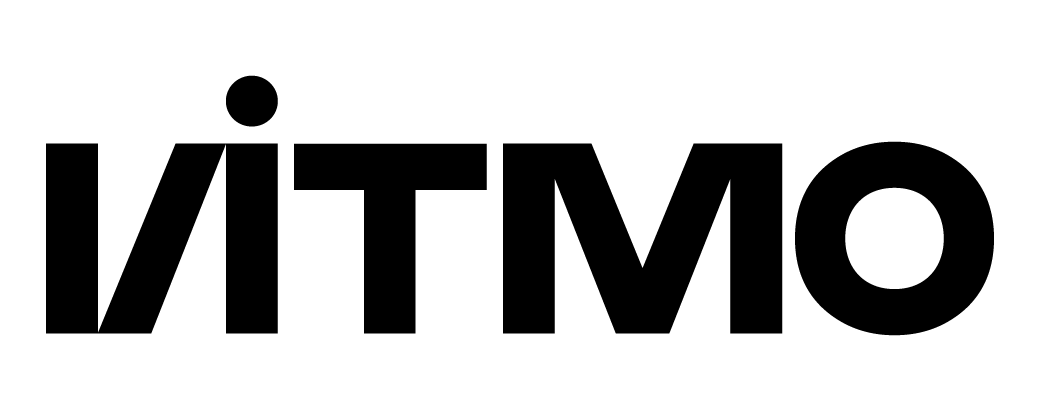
\includegraphics[width=0.3\linewidth]{label.png}
\end{figure}
\vspace{0.5cm}
\large Факультет информационных технологий и программирования\\

\vspace{1.5cm}

\textbf{\fontsize{60pt}{0}\selectfont{ОТЧЕТ}}\\
\vspace{0.5cm}
по лабораторной работе №2\\
\vspace{0.5cm}
на тему:\\
\vspace{0.5cm}
\textbf{\enquote{Градиентный спуск: классика}}


\begin{flushright}
Работу выполнили студенты\\
Группы M3233\\
Калиновский Арсений Владимирович\\
Рудаков Максим Андреевич\\
\end{flushright}
    
\includegraphics[width=.76\linewidth]{image.png}
\vfill

Санкт-Петербург\\  
\today

\end{center}
\end{titlepage}

\section{Цели работы}
Изучение различных алгоритмов градиентного спуска поиска минимума многомерных функций функций, в том числе:
\begin{enumerate}
    \item Эффективность их работы,
    \item Особенности поведения для различных задач (разные функции, приемлемая погрешность),
    \item Скорость сходимости,
    \item Вычислительные потребности.
\end{enumerate}

\section{Задачи, решаемые при выполнении работы}
\begin{enumerate}
    \item Реализация основных алгоритмов градиентного спуска,
    \item Анализ работы алгоритмов при различных конфигурациях работы,
    \item Изучение особенностей работы алгоритмов в разных сценариях.
\end{enumerate}

\section{Объект исследования}
Оптимизаторы многомерных функций методом градиентного спуска

\section{Модели задач}

\begin{enumerate}
    \item Хорошо обусловленная выпуклая квадратичная функция $f (x, y) = x^2 + y^2$.
    \item Плохо обусловленная выпуклая квадратичная функция $g(x, y) = x^2 + 100y^2$.
    \item Сложные функции: Розенброка, Экли, Химмельблау
\end{enumerate}

\section{Структура проекта}
Проект состоит из 3 частей:
\begin{enumerate}
    \item Модуль \t{optimizers}, в котором содержится реализация всех оптимизаторов,
    \item Файл \t{functions.py}, в котором содержатся описания основных функций,
    \item Функция $\t{main}$, которая отвечает за вызов оптимизаторов, сбор данных и введение статистики (таблицы, графики).
\end{enumerate}

Все оптимизаторы реализуют базовый класс $\texttt{optimizer\_base}$, в котором объявлен абстрактный метод $\texttt{find\_minimum}$, отвечающий за поиск минимума. От него унаследован ещё один базовый класс $\texttt{grad\_descent\_base}$, в котором объявлена функция $\texttt{iteration\_impl}$, отвечающая за итерацию алгоритма. Наследниками $\texttt{active\_search\_base}$ являются:
\begin{enumerate}
    \item $\t{grad\_descent\_cnst}$, реализующий градиентный спуск с постоянным шагом,
    \item $\t{grad\_descent\_armijo}$, реализующий градиентный спуск методом дробления шага (с условием Армихо),
    \item $\t{grad\_descent\_wolfe}$, реализующий градиентный спуск методом дробления шага (с сильными условиями Вольфе),
    \item $\t{grad\_descent\_steepest}$, реализующий градиентный спуск методом наискорейшего градиентного спуска.
\end{enumerate}

Результаты выполнения функции $\t{main}$ распределены в зависимости от задания по разным папкам, которые имеют названия $\t{task1-6}$. В названии каждого файла явно указаны метод и оптимизируемая функция, а также некоторая дополнительная информация, которая может иметь значение для конкретного задания.

В рамках лабораторной работы в качестве условия на остановку использовалось условие на норму градиента. Тем не менее, оптимизаторы написаны таким образом, что можно в качестве условия на остановку выбрать либо разность значений функций в соседних точках, либо норму вектора-разности.

\section {Оптимизируемые функции}
В данном разделе будут приведены определения оптимизируемых функций.
\subsection{Хорошо обусловленная выпуклая квадратичная функция $f (x, y)$}
В рамках этой лабораторной работы в качестве \enquote{хорошей} функции используется функция $f(x, y) = x^2 + y^2$. Заметим, что у неё есть четко выделенный минимум в точке (0,0), а её поведение максимально симметрично, что неудивительно, ведь её линии уровня представляют собой концентрические окружности с центром в той самой точке минимума.  Её градиент $\nabla f$ имеет вид $(2x, 2y)$.
\subsection{Плохо обусловленная выпуклая квадратичная функция $g(x, y)$}
В рамках этой лабораторной работы в качестве \enquote{плохой} функции используется функция $g(x, y) = x^2 + 100 \cdot y^2$. Линии уровня этой функции есть сильно вытянутые вдоль оси $OX$ эллипсы. Таким образом, для этой функции характерна сильная асимметрия. Её градиент $\nabla g$ имеет вид $(2x, 200y)$.

Заметим, что приведенные выше функции являются выпуклыми.
\subsection{Сложные функции}
В рамках данной лабораторной работы использованы следующие \enquote{сложные функции}:
\begin{itemize}
    \item Функция Розенброка $\rho(x,y) = (1 - x)^2 + 100(y - x^2)^2$. У неё единственный минимум 0 в точке (1,1). Заметим, что функция Розенброка не является выпуклой. Её градиент $\nabla \rho$ имеет вид $(-2(1 - x) - 400 x (y - x ^2), 200 (y - x^2))$.
    \begin{figure}[H]
        \centering
        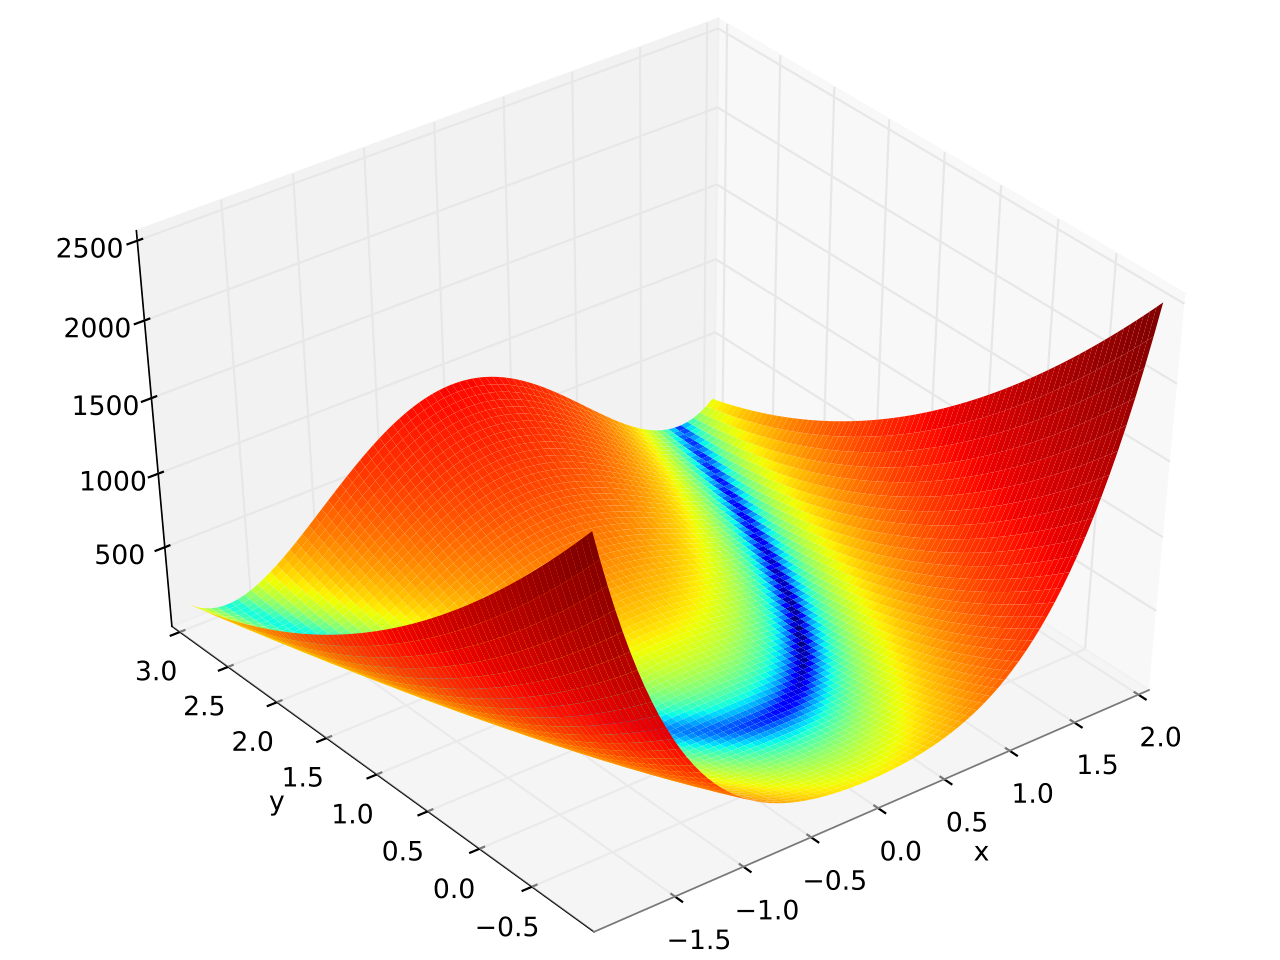
\includegraphics[width=0.5\linewidth]{rosenbrock.png}
        \caption{График функции Розенброка.}
    \end{figure}
    \item Функция Экли, имеющая вид:
    \begin{equation*}
        \textbf{A}(x,y) = -20 \exp\left[ -0.2\sqrt{\frac12 \left(x^2 + y^2 \right)}\right]
    \end{equation*}
    \begin{equation*}
        - \exp \left[ \frac12 (\cos(2\pi x) + \cos (2\pi y))\right] + e + 20.
    \end{equation*}
    Её градиент:
    \begin{equation*}
        \nabla \textbf{A}_{x_i} =  \frac{\left(2 x_i \exp\left[ \frac12 \left(x^2 + y^2 \right)\right]\right)}{\sqrt{\frac12 \left(x^2 + y^2 \right)}} + \pi\sin(2 \pi x_i) \cdot \exp\left[\frac12 (\cos(2\pi x) + \cos (2\pi y)) \right]
    \end{equation*}
    \begin{equation*}
        x_i \in \{x, y\}.
    \end{equation*}
    У данной функции есть единственный глобальный минимум в точке (0, 0). Она характеризуется своей хаотичностью и часто используется для исследования производительности алгоритмов минимизации.
    \begin{figure}[H]
        \centering
        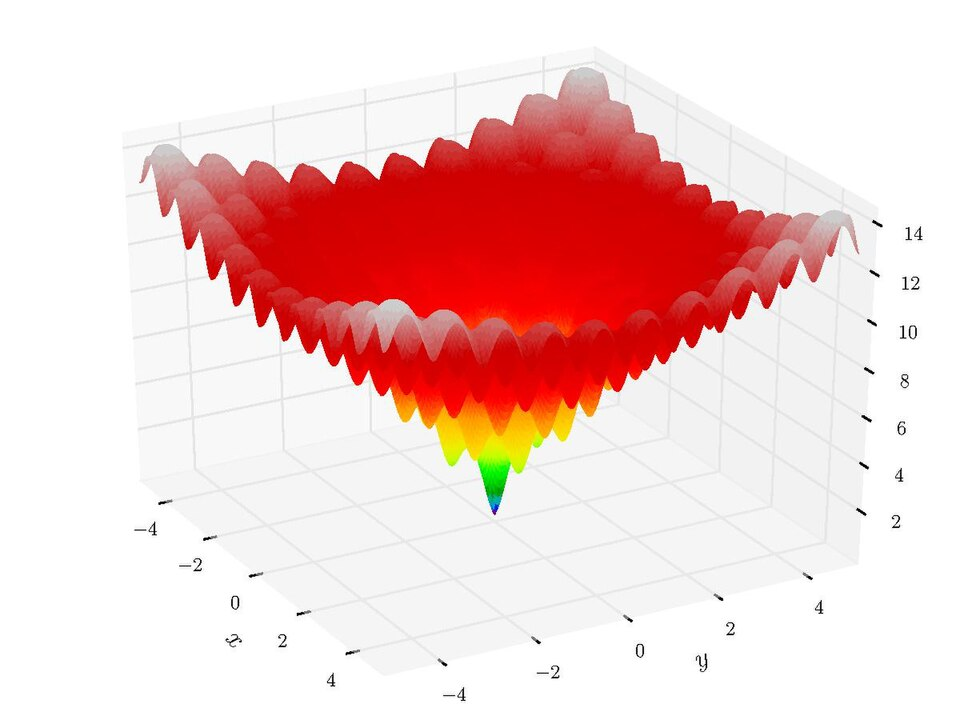
\includegraphics[width=0.5\linewidth]{ackley.png}
        \caption{График функции Экли.}
    \end{figure}
    \item Функция Химмельблау, равная $\xi (x, y) = (x ^ 2 + y - 11)^2 + (x + y^2 -y)^2$. Эта функция характеризуется наличием трёх равнозначных локальных минимумов, в каждом из которых функция принимает значение 0. Эти минимумы соответственно имеют вид (3,2), (-2.805$\ldots$, 3.131$\ldots), (-3.779$\ldots, -3.283$\ldots$), (3.584$\ldots$, -1.848$\ldots$). Её градиент имеет вид:
    \begin{equation*}
        \nabla \xi (x, y) = (4x(x^2 + y - 11) + 2(x + y^2 - 7), 2(x^2 + y - 11) + 4y(x + y^2 - 7)).
    \end{equation*}
    \begin{figure}[H]
        \centering
        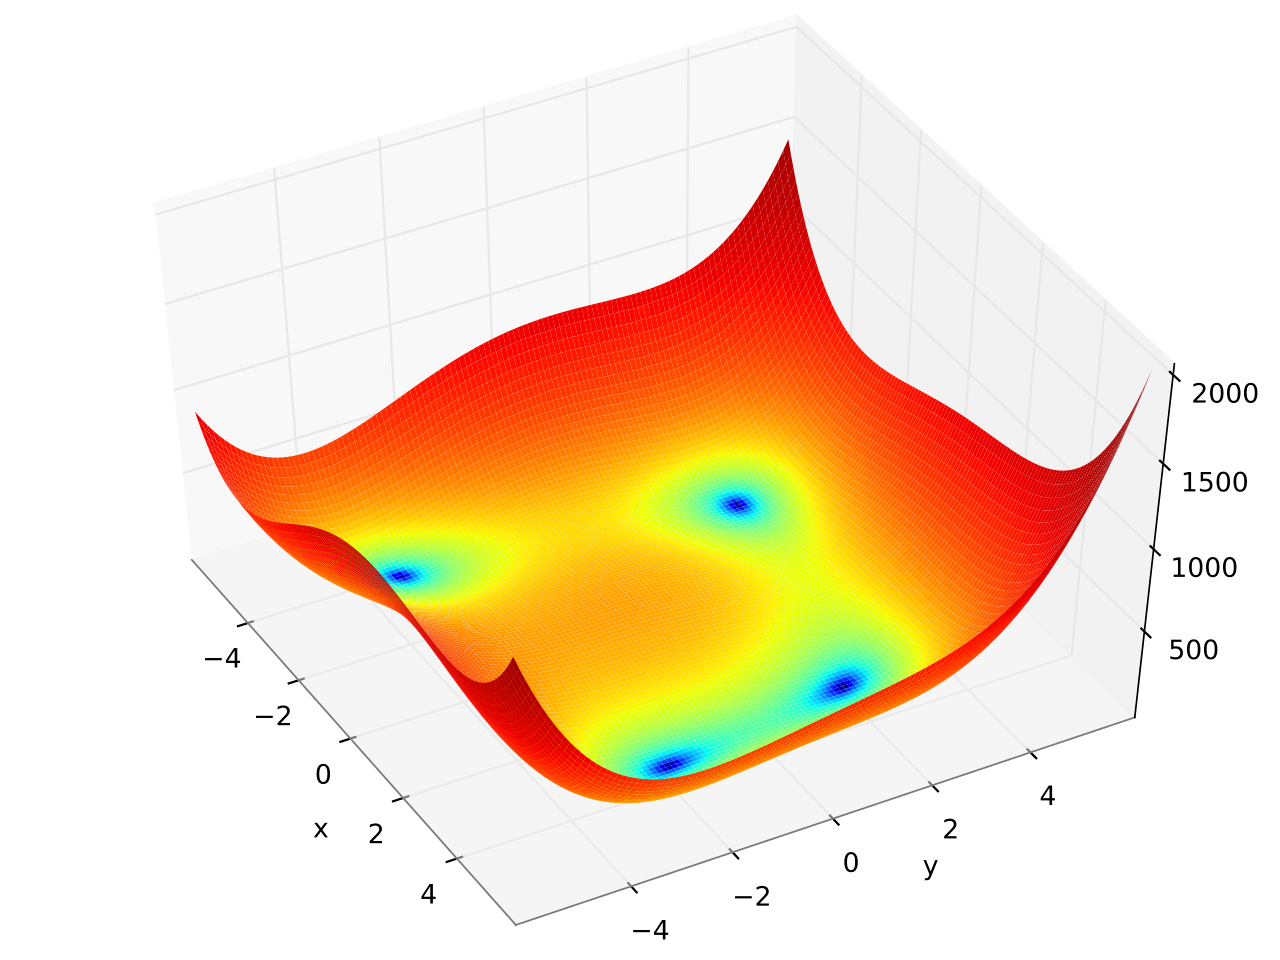
\includegraphics[width=0.5\linewidth]{himmelblau.png}
        \caption{График функции Химмельблау}
    \end{figure}
\end{itemize}

\section{Теория}
Пусть имеется многомерная функция $f : D \subseteq \mathbb{R}^n \rightarrow \mathbb{R}$, у который есть точка минимума $x^*$. Заметим, что итерационный процесс можно описать последовательностью $\{x_k\}_{i=1}^{\infty}$, в которой $x_{k+1} = x_k + \alpha_k p_k$, где $\alpha_k$ -- скаляр, а $p_k$ -- вектор. Таким образом, для нахождения минимума достаточно найти такие $\alpha_k, p_k$, что последовательность векторов $x_k$ сходятся к точке минимума функции.

Методом градиентного спуска называется метод, в котором направление $p_k$ фиксировано и равно антиградиенту функции в точке $x_k$: $p_k = - \nabla f(x_k)$. Таким образом, для нахождения минимума остается найти только последовательность $\alpha_k$.

Методом градиентного спуска с постоянным шагом называется метод, в котором в качестве $\alpha_k$ используется ранее выбранная константа.

Методом градиентного спуска с дроблением шага называется метод, в котором  $\alpha_k$ выбирается на каждом шаге итерации алгоритма таким образом, чтобы соблюдалось некоторе условие на функцию (Армихо, сильное условие Вольфе).

Говорят, что выполняется условие Армихо, если
\begin{equation*}
    f(x_k + \alpha_k p_k) \leq f(x_k) - c_1 \alpha_k \|\nabla f(x_k)\|^2.
\end{equation*}

Говорят, что выполняется сильные условия Вольфе, если выполнено условие Армихо и
\begin{equation*}
    |\nabla f(x_k + \alpha_k p_k) \cdot p_k| \leq c_2 \|\nabla f(x_k)\|^2, 0 < c_1 < c_2 < 1.
\end{equation*}


Методом наискорейшего градиентного спуска называется метод, в котором в качестве $\alpha_k$ выбирается из условия:
\begin{equation*}
    \alpha_k \in \underset{\alpha \geq 0}{f(x_k + \alpha p_k)}.
\end{equation*}

\section{Анализ результатов}
\subsection{Сходимость метода с постоянным шагом}
\subsubsection{Сходимость метода с постоянным шагом для квадратичных функций}

В рамках опыта использовалось ограничение на количество итераций (не более миллиона итераций) и начальная точка (2, 2).

При исследовании метода градиентного спуска с постоянным шагом на каждой квадратичной функции были получены следующие результаты:
\begin{table}[!ht]
    \centering
    \resizebox{\textwidth}{!}{
    \begin{tabular}{|S|c|S|S|S|}
    \hline
        {Step} & {N\_Iter} & {X\_min\_x} & {X\_min\_y} & {F\_min} \\ \hline
        0.1 & 92 & 3.035420144102704e-09 & 3.035420144102704e-09 & 1.8427550902448958e-17 \\ \hline
        0.01 & 999 & 3.5047216934942795e-09 & 3.5047216934942795e-09 & 2.456614829769882e-17 \\ \hline
        0.001 & 10068 & 3.5333701487051693e-09 & 3.5333701487051693e-09 & 2.496940921552158e-17 \\ \hline
        0.0001 & 100759 & 3.5352979756912692e-09 & 3.5352979756912692e-09 & 2.4996663553853572e-17 \\ \hline
        1e-05 & 1000000 & 4.121565286183822e-09 & 4.121565286183822e-09 & 3.397460081655107e-17 \\ \hline
        1e-06 & 1000000 & 0.2706705664730416 & 0.2706705664730416 & 0.14652511110967448 \\ \hline
    \end{tabular}}
    \caption{Результаты для хорошей функции.}
\end{table}

\begin{table}[!ht]
    \centering
    \resizebox{\textwidth}{!}{  
    \begin{tabular}{|S|c|S|S|S|}
    \hline
        {Step} & {N\_Iter} & {X\_min\_x} & {X\_min\_y} & {F\_min} \\ \hline
        0.1 & 243 & 7.060034896770557e-24 & NaN & NaN \\ \hline
        0.01 & 1000000 & 1.2e-322 & -2.0 & 400.0 \\ \hline
        0.001 & 9895 & 4.995805167810676e-09 & 1e-323 & 2.4958069274723862e-17 \\ \hline
        0.0001 & 99026 & 4.9999717049099474e-09 & 1.2e-322 & 2.4999717049900087e-17 \\ \hline
        1e-05 & 990340 & 4.999985173178659e-09 & 1.23e-321 & 2.4999851732006424e-17 \\ \hline
        1e-06 & 1000000 & 0.2706705664730416 & 2.713522547803834e-87 & 0.07326255555483724 \\ \hline
    \end{tabular}}
    \caption{Результаты для плохой функции.}
\end{table}

\begin{figure}[H]
    \centering
    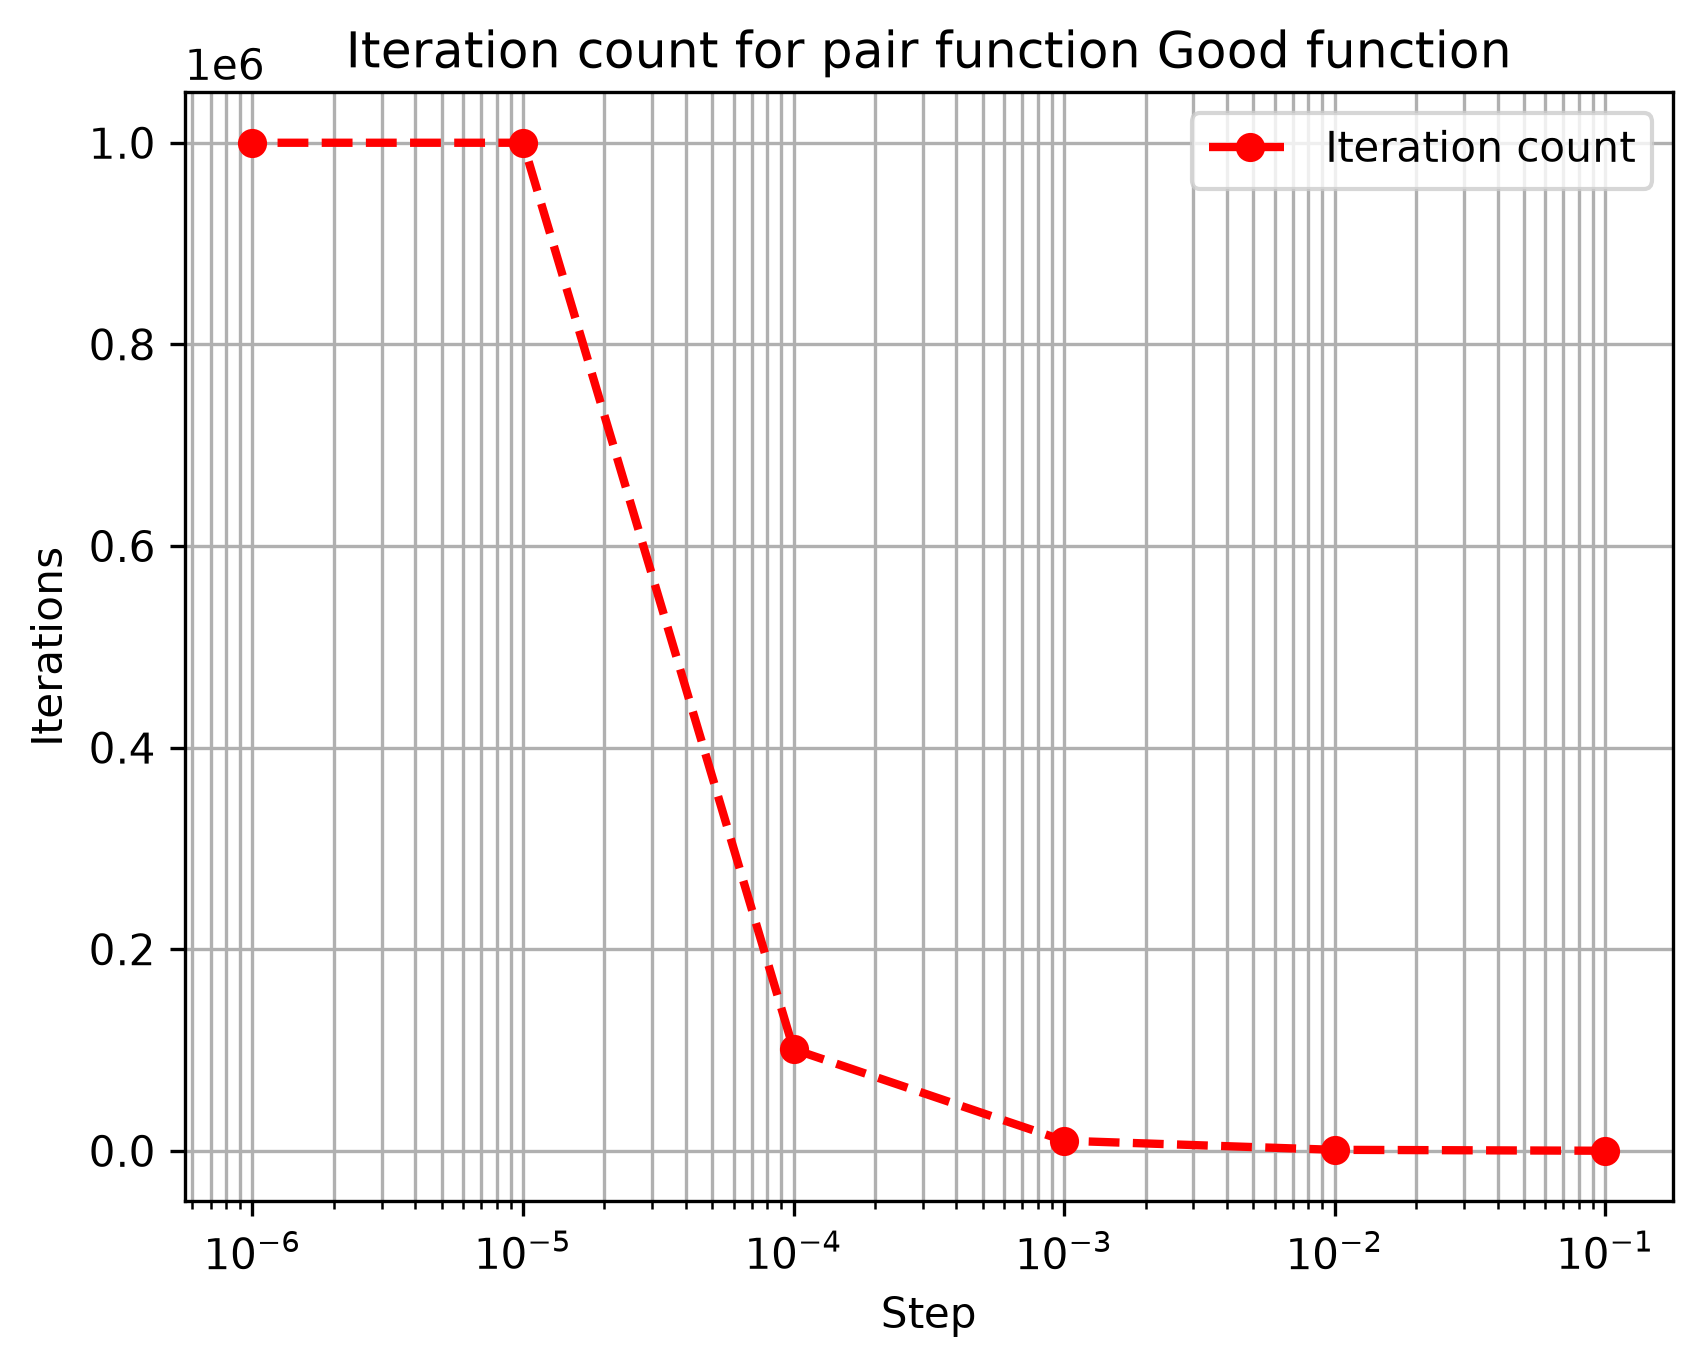
\includegraphics[width=0.75\linewidth]{task1_Step_Good function_plot.png}
    \caption{Результаты для хорошей функции.}
\end{figure}

\begin{figure}[H]
    \centering
    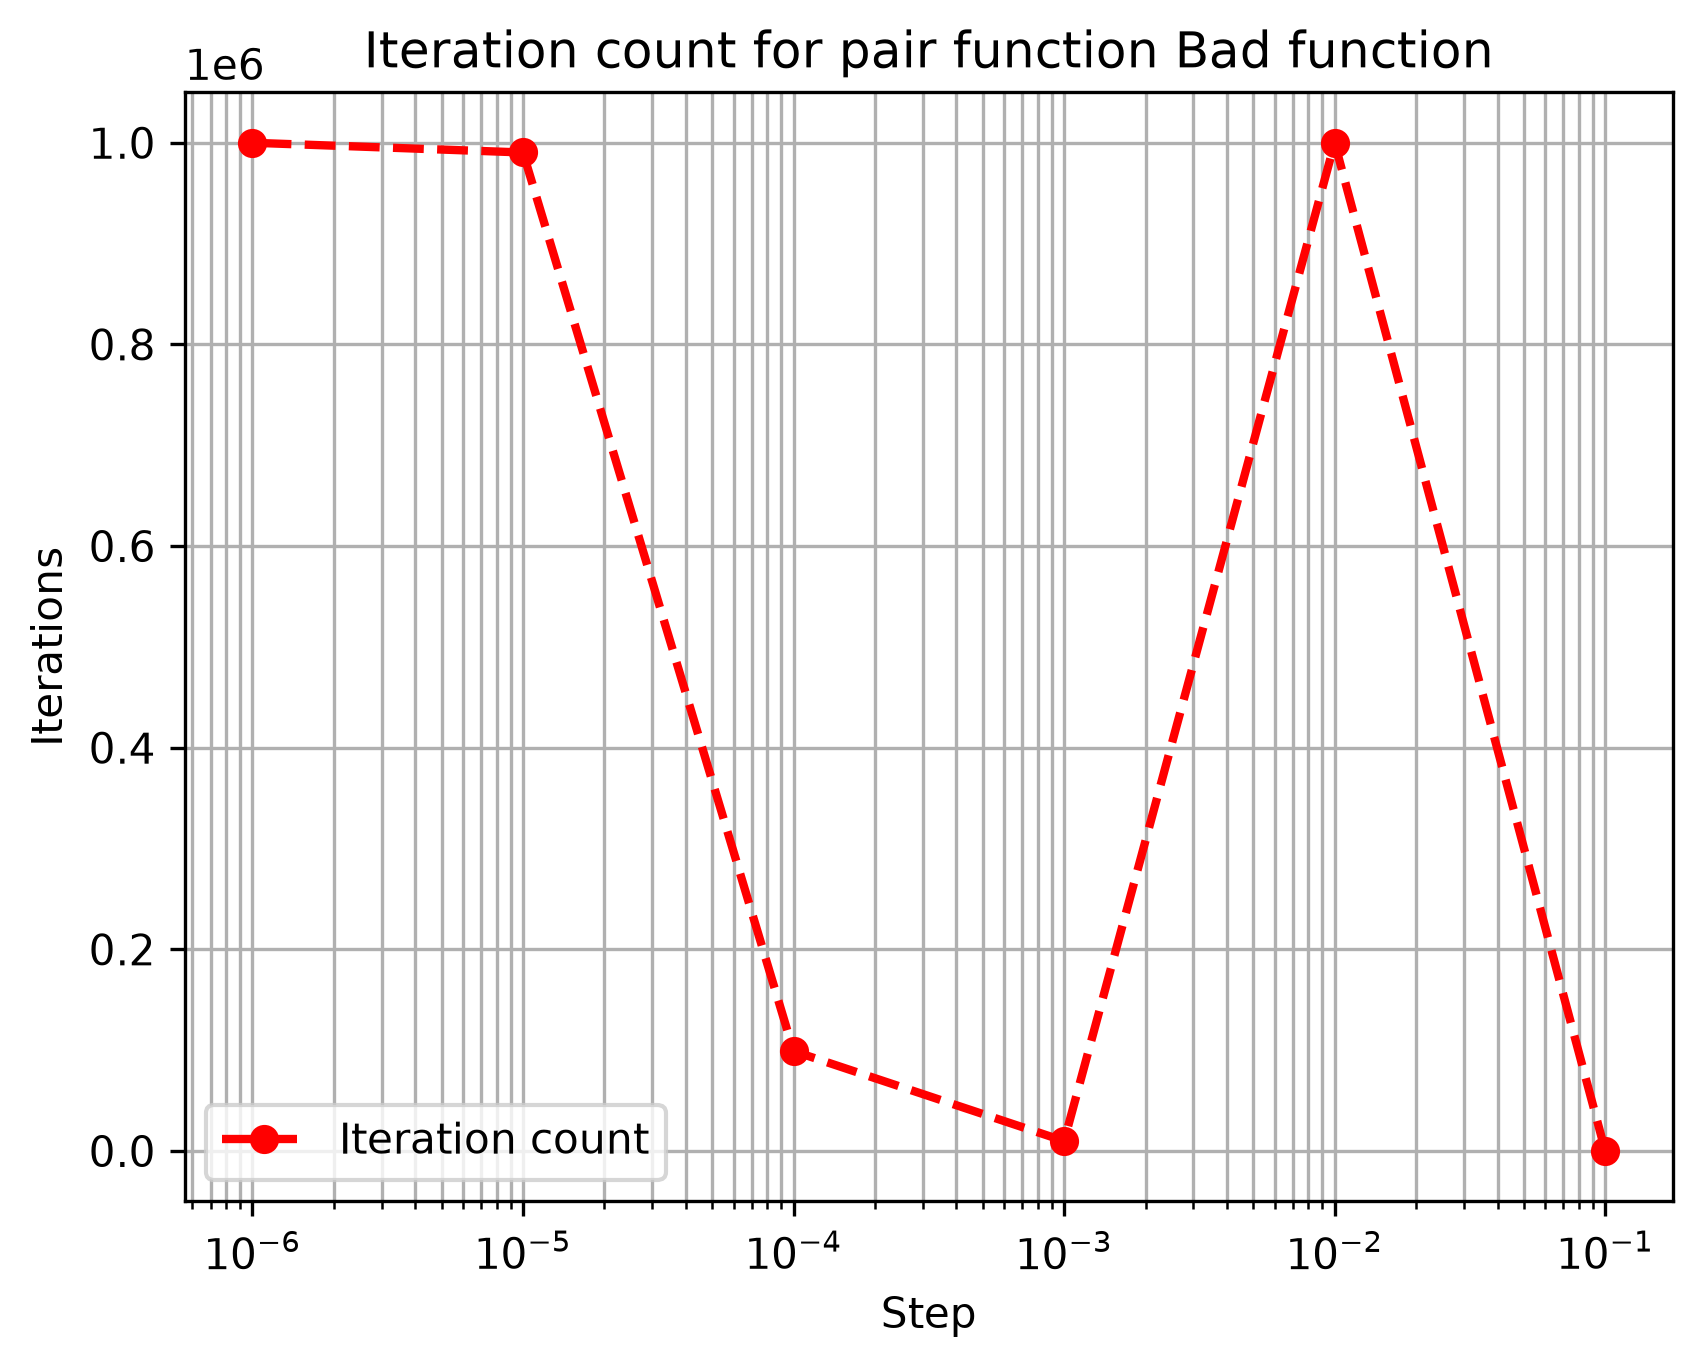
\includegraphics[width=0.75\linewidth]{task1_Step_Bad function_plot.png}
    \caption{Результаты для плохой функции.}
\end{figure}

Видно, что для хорошей функции число итераций обратно пропорционально требуемой точности. Это логично, ведь чем ближе алгоритм к минимуму, тем меньше градиент и тем медленнее происходит приближение к требуемому минимуму.

Похожим образом алгоритм ведет себя для плохой функции: начиная со значения шага $10^{-3}$, количество шагов растет обратно пропорционально величине шага. Однако для малых величин шага алгоритм ведет себя хаотично. У этого есть объяснение: для величины шага $0.1$ алгоритм \enquote{прыгает} вдоль оси $OX$, с каждым шагом оказываясь дальше от начала координат. А чем дальше точка от начал, тем больше модуль градуента. Таким образом, алгоритм \enquote{накапливает импульс}, быстро достигая величин порядка бесконечности, после чего выполняет сложение бесконечностей разных знаков и останавливается преждевременно. Для величины шага $0.01$ ситуация обратная: алгоритм хотя и делает достаточно большие шаги для того, чтобы перемещаться туда-сюда вдоль оси $OX$, этих шагов недостаточно, чтобы \enquote{набрать импульса}, в результате чего совершаются колебания относительно начала координат.

Следующие два графика траекторий движения демонстрируют работу алгоритма (шаг $0.001$):

\begin{figure}[H]
    \centering
    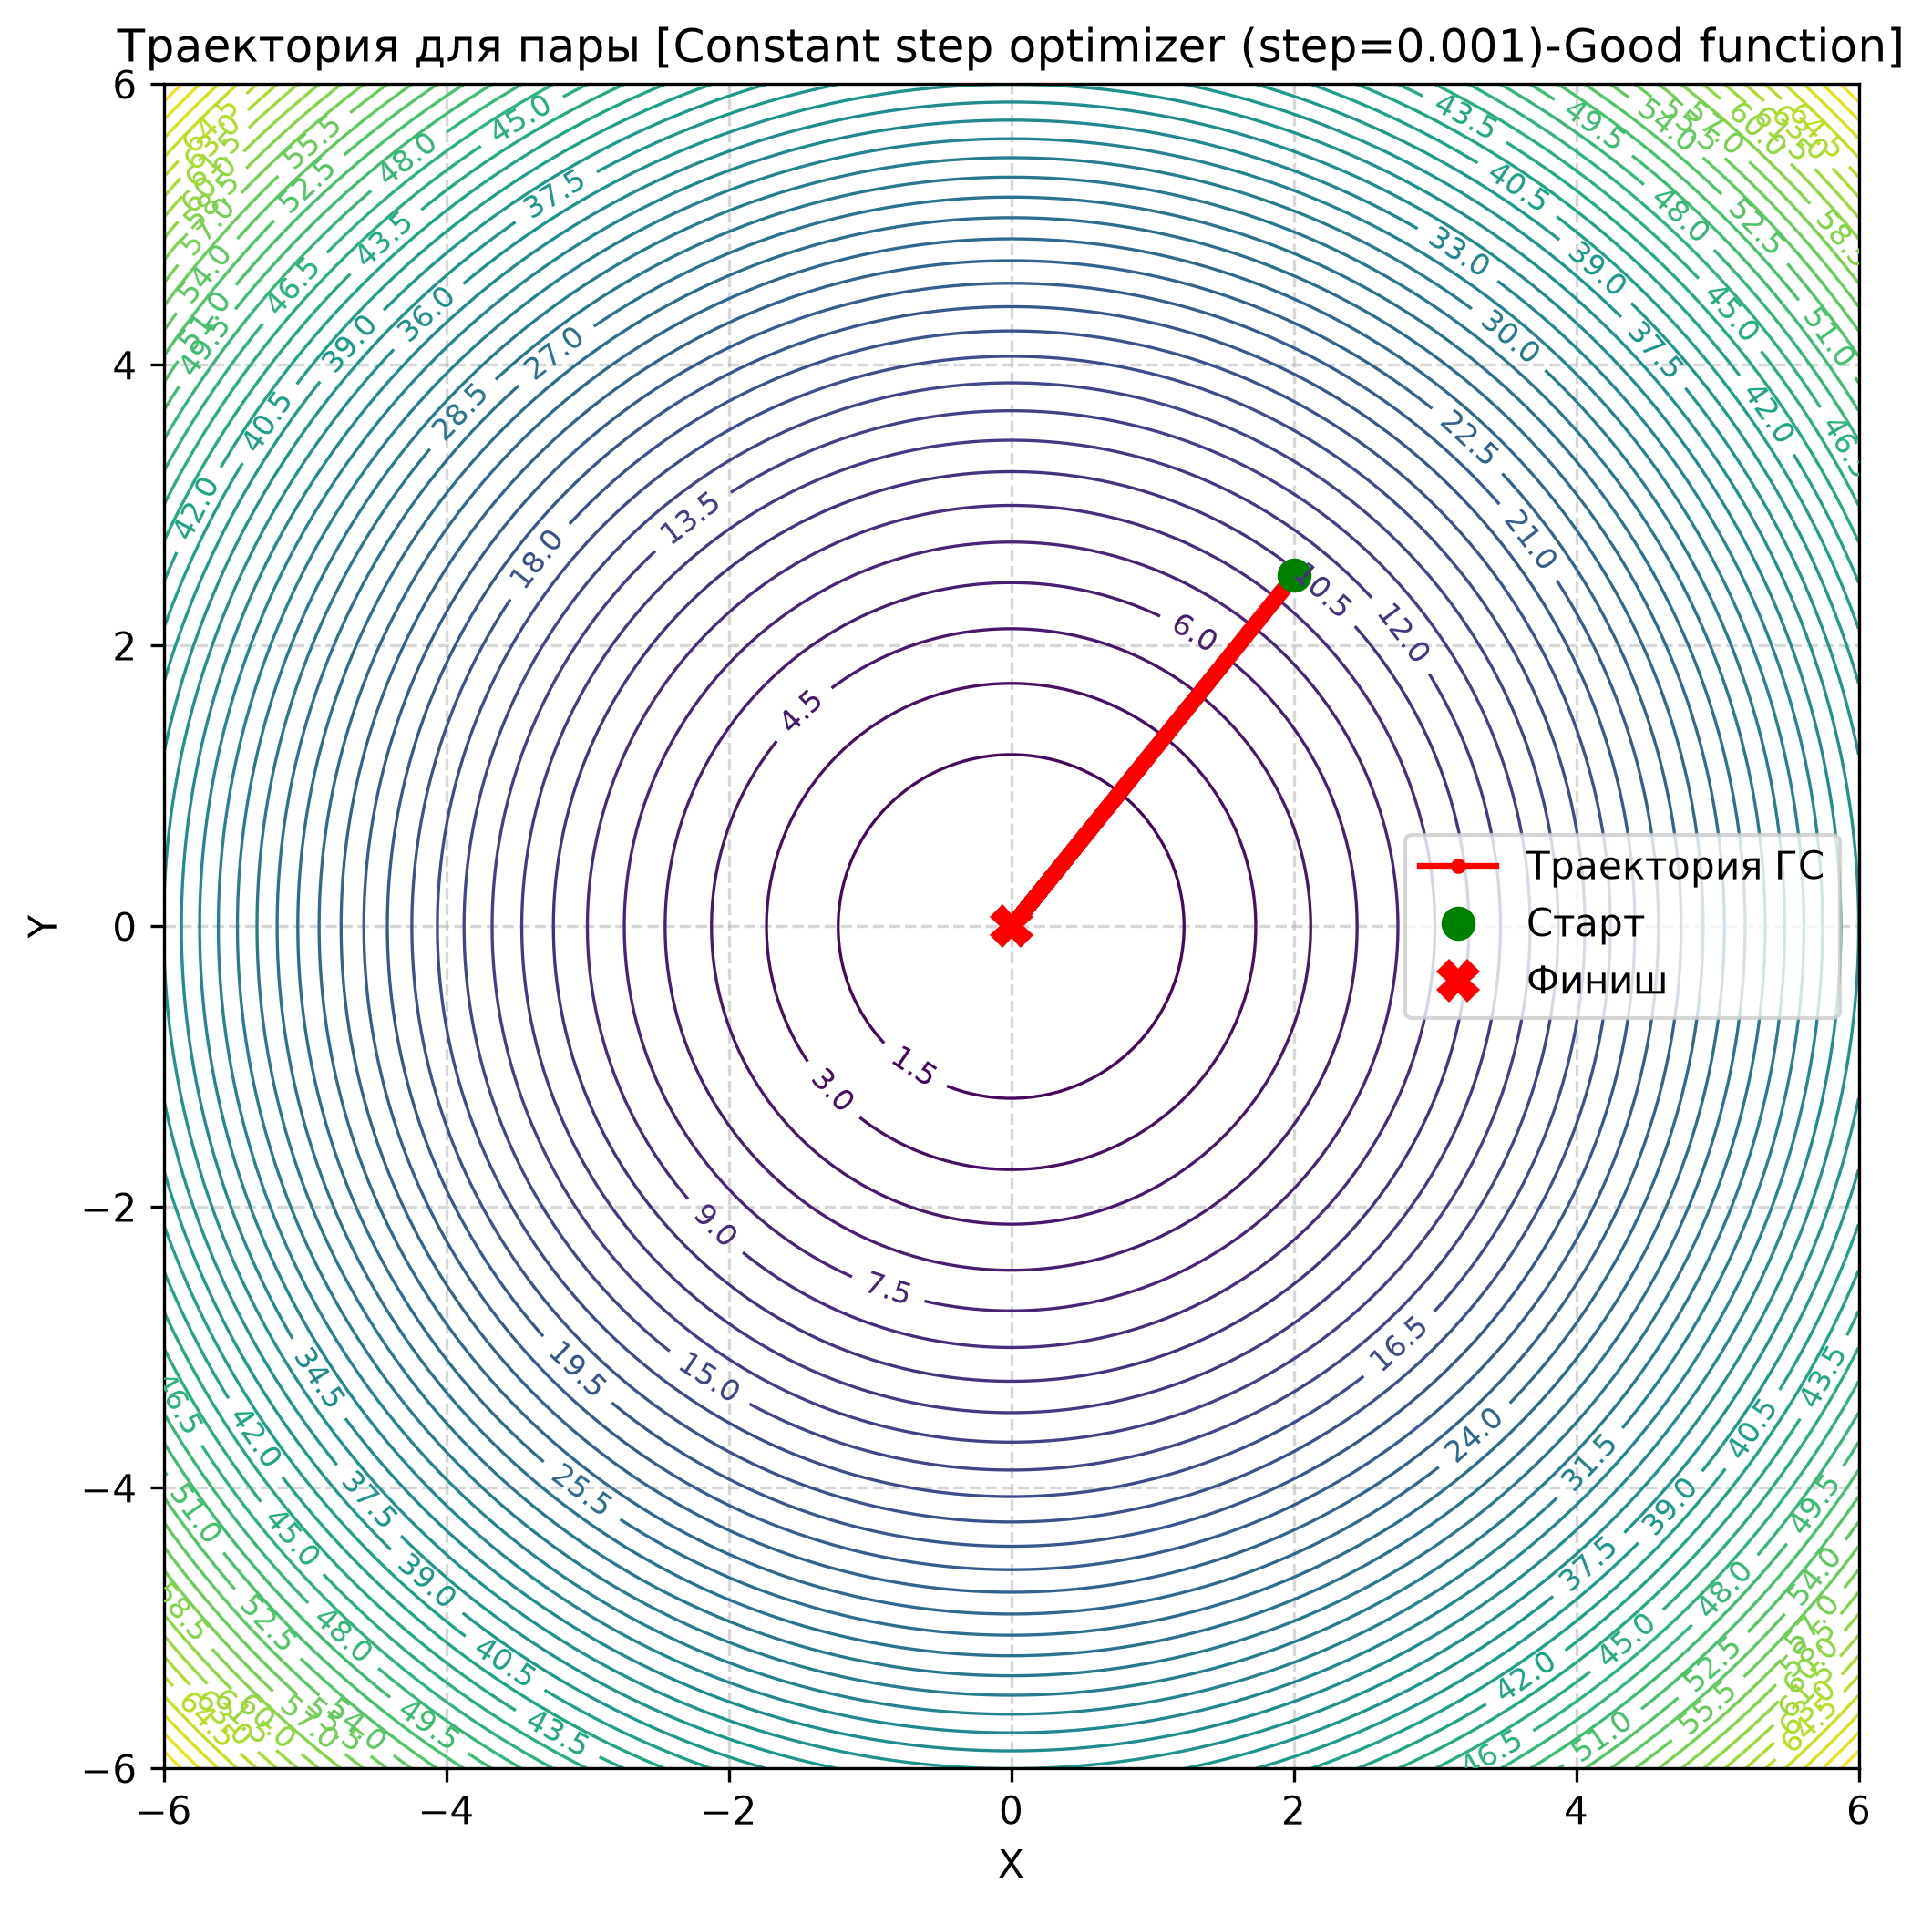
\includegraphics[width=1\linewidth]{plot_[Constant step optimizer (step=0.001)-Good function]__Trajectory.png}
    \caption{Траектория движения для хорошей функции. }
\end{figure}
\begin{figure}[H]
    \centering
    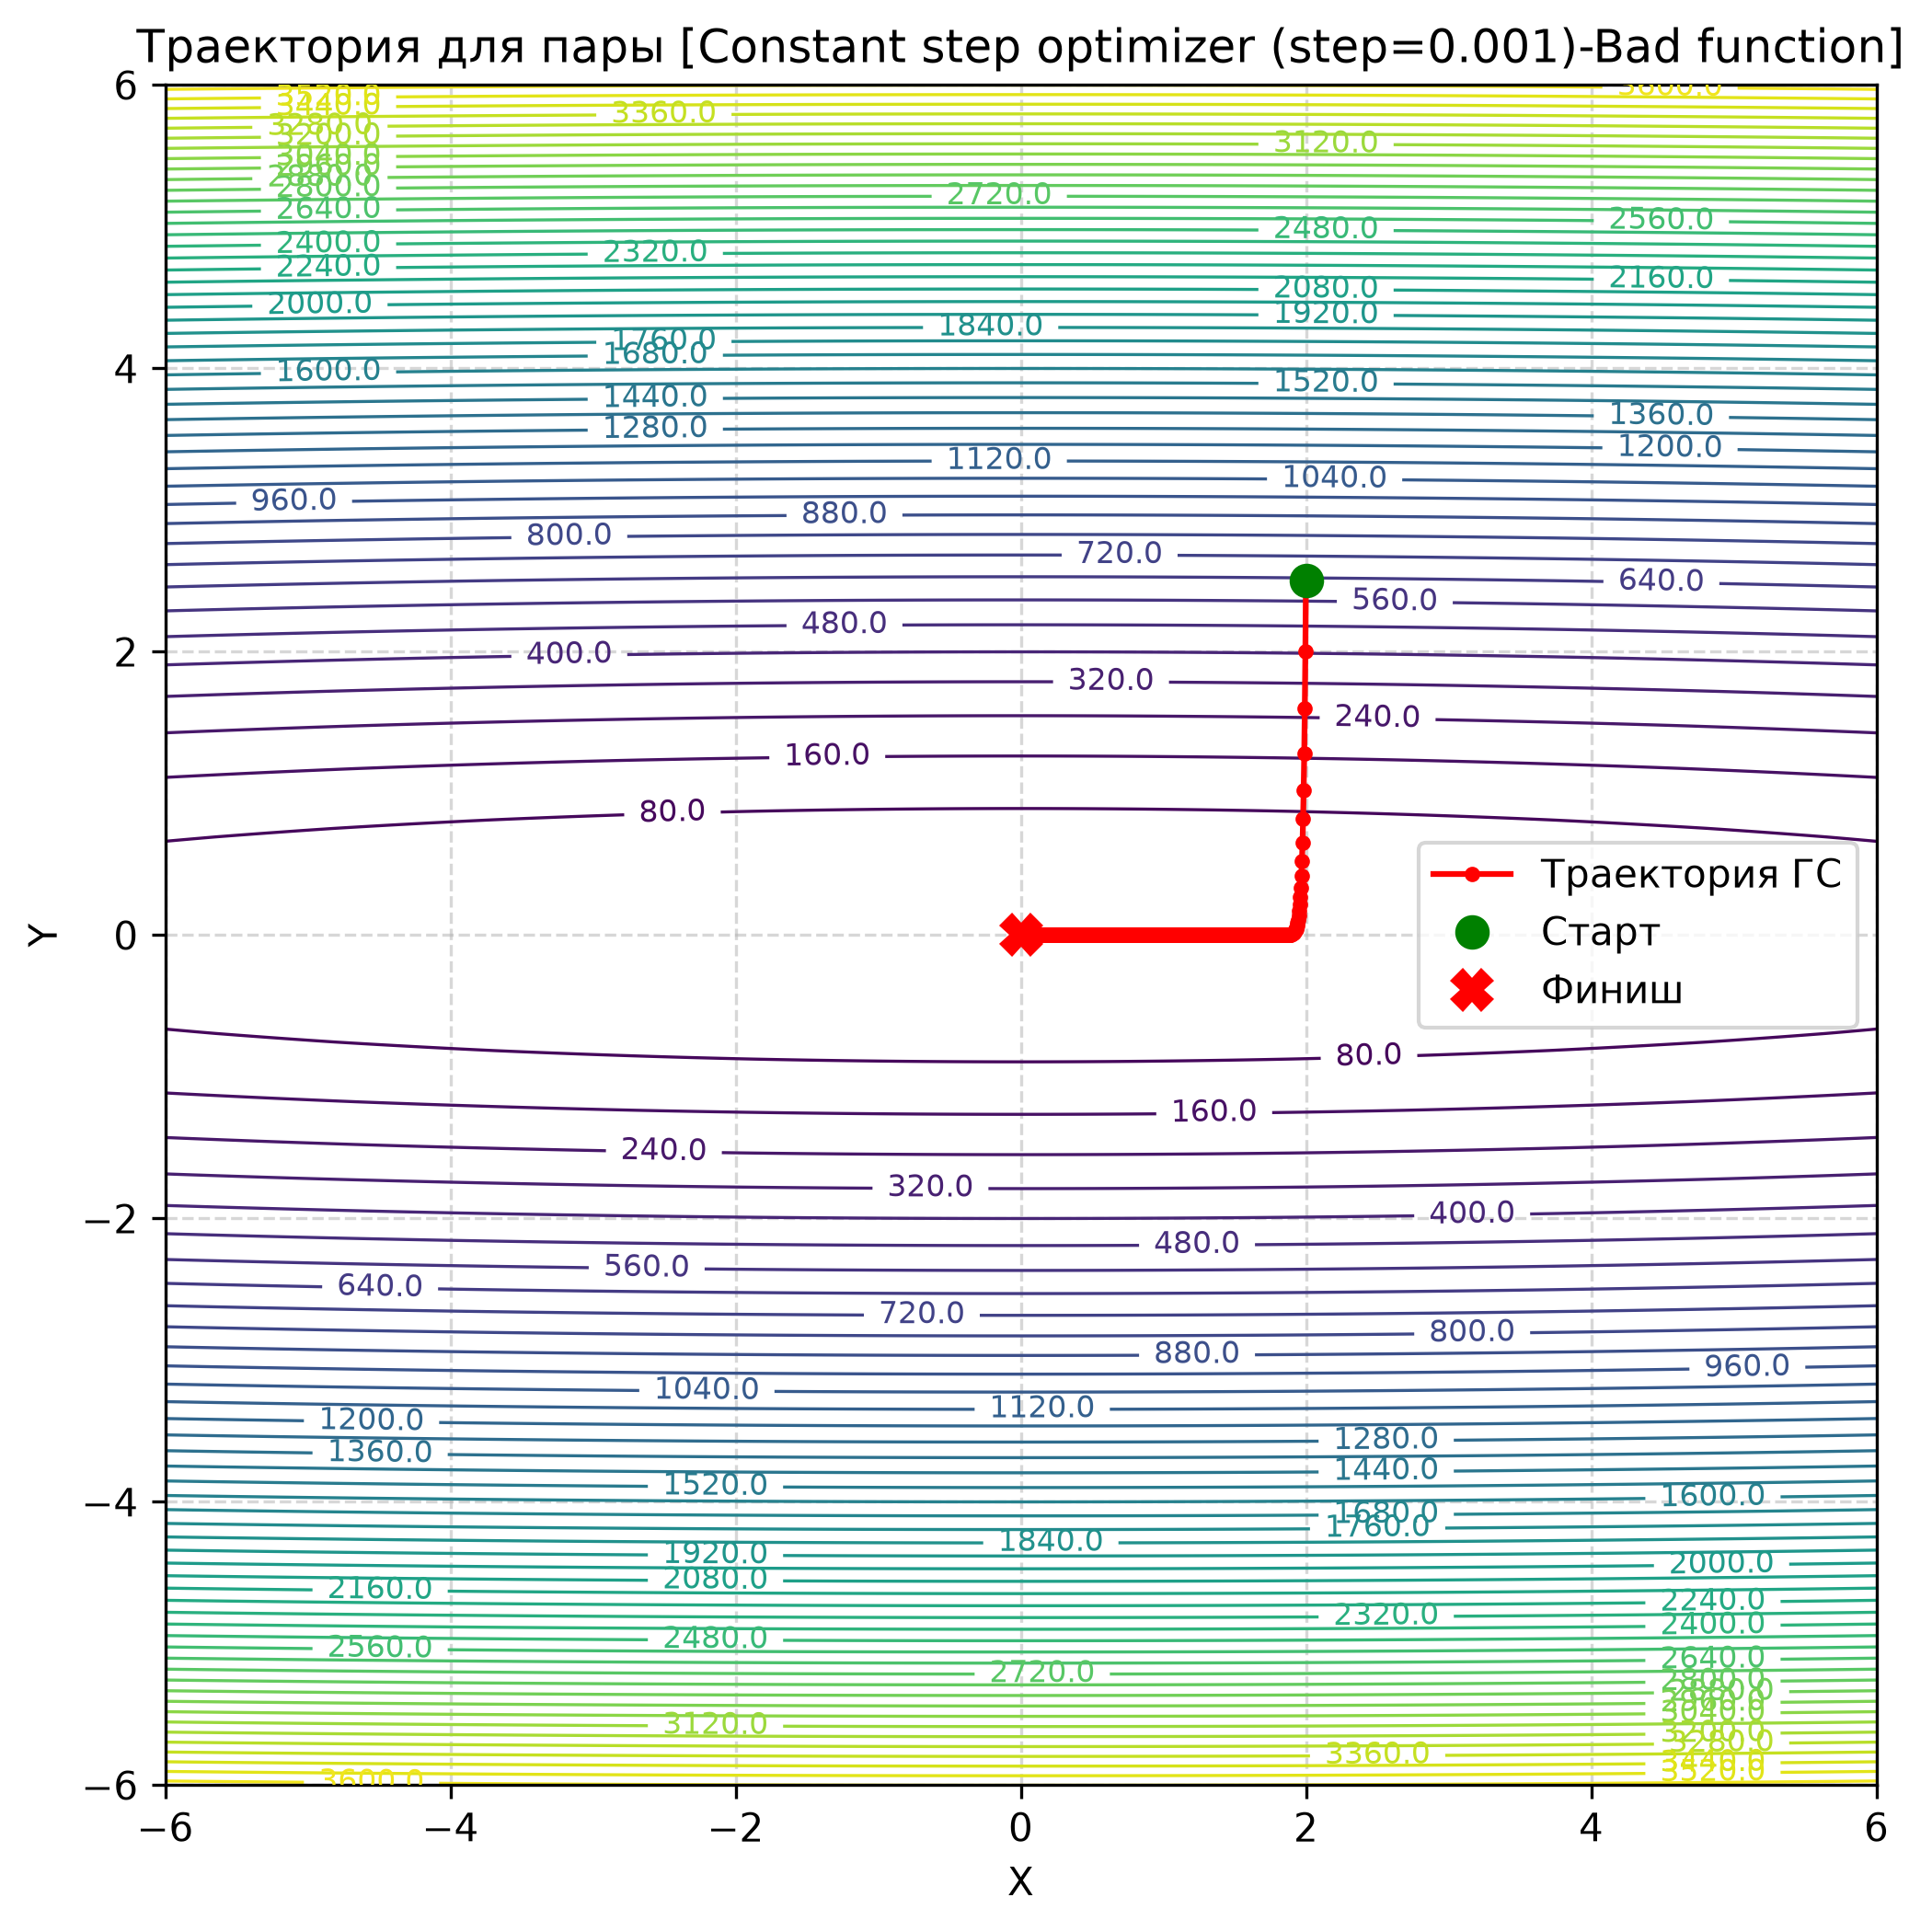
\includegraphics[width=0.6\linewidth]{plot_[Constant step optimizer (step=0.001)-Bad function]__Trajectory.png}
    \caption{Траектория движения для хорошей функции.}
\end{figure}

\subsubsection{Сходимость метода с постоянным шагом для сложных функций}

В рамках опыта использовалось ограничение на количество итераций (не более 100000 итераций) и начальная точка (2, 2).

\begin{table}[!ht]
    \centering
    \resizebox{\textwidth}{!}{  
    \begin{tabular}{|S|c|S|S|S|}
    \hline
        {Step} & {N\_Iter} & {X\_min\_x} & {X\_min\_y} & {F\_min}\\ \hline
        0.1 & 100000 & 0.3722967403900969 & 0.3722967403900969 & 3.6543007688503373 \\ \hline
        0.01 & 28 & 1.9744519866060186 & 1.9744519866060186 & 6.559645375627877 \\ \hline
        0.001 & 367 & 1.9744519866167545 & 1.9744519866167545 & 6.5596453756278805 \\ \hline
    \end{tabular}
    }
    \caption{Результаты для функции Экли.}
\end{table}

\begin{table}[!ht]
    \centering
    \resizebox{\textwidth}{!}{  
    \begin{tabular}{|S|c|S|S|S|}
    \hline
        {Step} & {N\_Iter} & {X\_min\_x} & {X\_min\_y} & {F\_min}\\ \hline
        0.1 & 9 & NaN & {-$\infty$} & NaN \\ \hline
        0.01 & 72 & 2.9999999998699503 & 2.000000000313968 & 1.4849399829843437e-18 \\ \hline
        0.001 & 804 & 2.999999999853159 & 2.0000000003545066 & 1.8931583890513092e-18 \\ \hline
    \end{tabular}
    }
    \caption{Результаты для функции Химмельблау.}
\end{table}

\begin{table}[!ht]
    \centering
    \resizebox{\textwidth}{!}{  
    \begin{tabular}{|S|c|S|S|S|}
    \hline
        {Step} & {N\_Iter} & {X\_min\_x} & {X\_min\_y} & {F\_min}\\ \hline
        0.1 & 7 & $\infty$ & $\infty$ & NaN \\ \hline
        0.01 & 8 & NaN & $\infty$ & NaN \\ \hline
        0.001 & 43803 & 1.0000000111778016 & 1.0000000224003325 & 1.2514331733232854e-16 \\ \hline
    \end{tabular}
    }
    \caption{Результаты для функции Розенброка.}
\end{table}

В случае функции Экли видно, что алгоритм находит лишь какой-то локальный минимум (коих у функции предостаточно), но тем не менее никогда не приближается к глобальному минимуму в точке (0,0). Это объясняется тем, что алгоритм, войдя в одну из \enquote{воронок} функции, никогда из неё не выбирает и ищет локальный минимум в этой воронке.

В случае функции Химмельблау видно, что для малых значений величины шага алгоритм, как в случае плохо обусловленной квадратичной функции, быстро удаляется от начала координат в бесконечность. Лишь при $\alpha \leq 0.01$ алгоритму удается найти один из глобальных минимумов в точке (3, 2). Логично, что алгоритм найдет именно этот минимум, ведь он ближе всех к начальной точке.

В случае случае Розенброка для мальх значений величины шага алгоритм опять-таки удаляется в сторону бесконечности. Тем не менее, при $\alpha = 0.001$ алгоритм удается найти глобальный минимум в точке (1, 1), используя при этом много итераций. Это объясняется тем, что функция имеет очень узкую и изогнутую долину, ведущую к минимуму в точке (1,1). При небольшом отклонении поперек этой долине алгоритм \enquote{перепрыгивает} её, оказываясь по другую сторону долины. Таким образом, алгоритм движется зигзагами, что объясняет такое медленное движение к минимуму.

Следующие три графика траекторий движения демонстрируют работу алгоритма (шаг $0.001$) для сложных функций:


\begin{figure}[H]
    \centering
    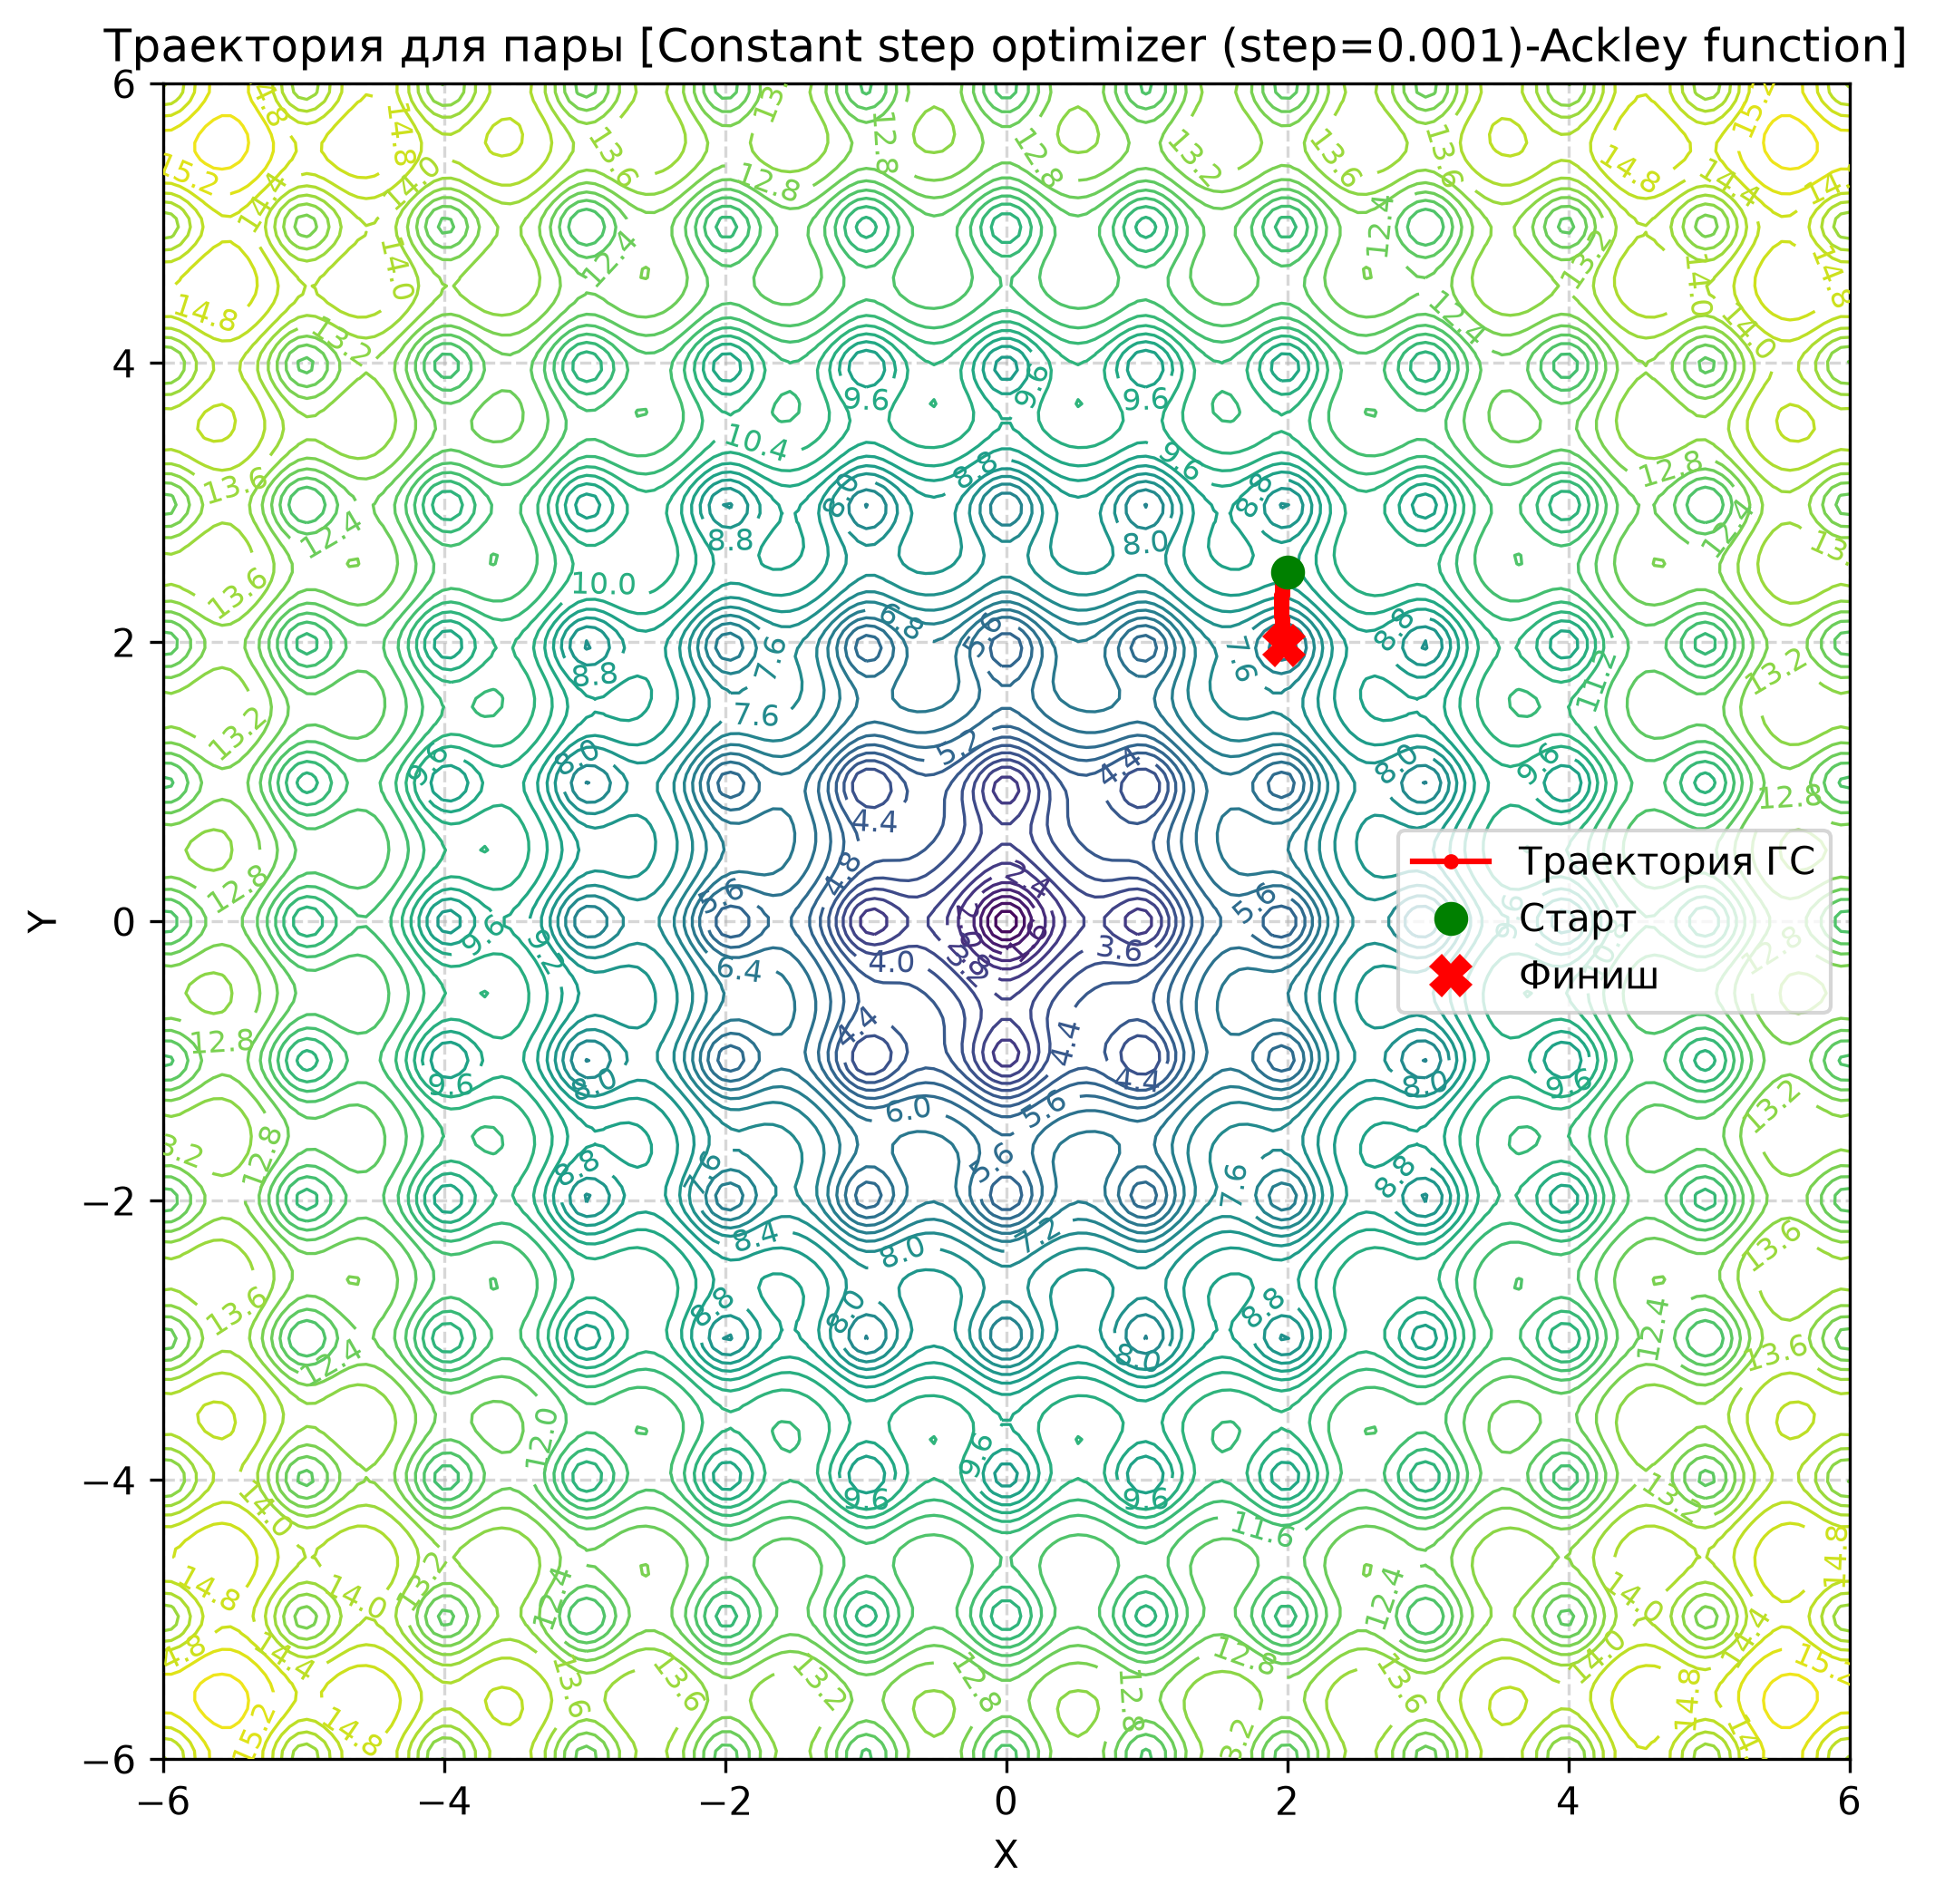
\includegraphics[width=0.7\linewidth]{plot_[Constant step optimizer (step=0.001)-Ackley function]__Trajectory.png}
    \caption{Траектория движения для функции Экли.}
\end{figure}
\begin{figure}[H]
    \centering
    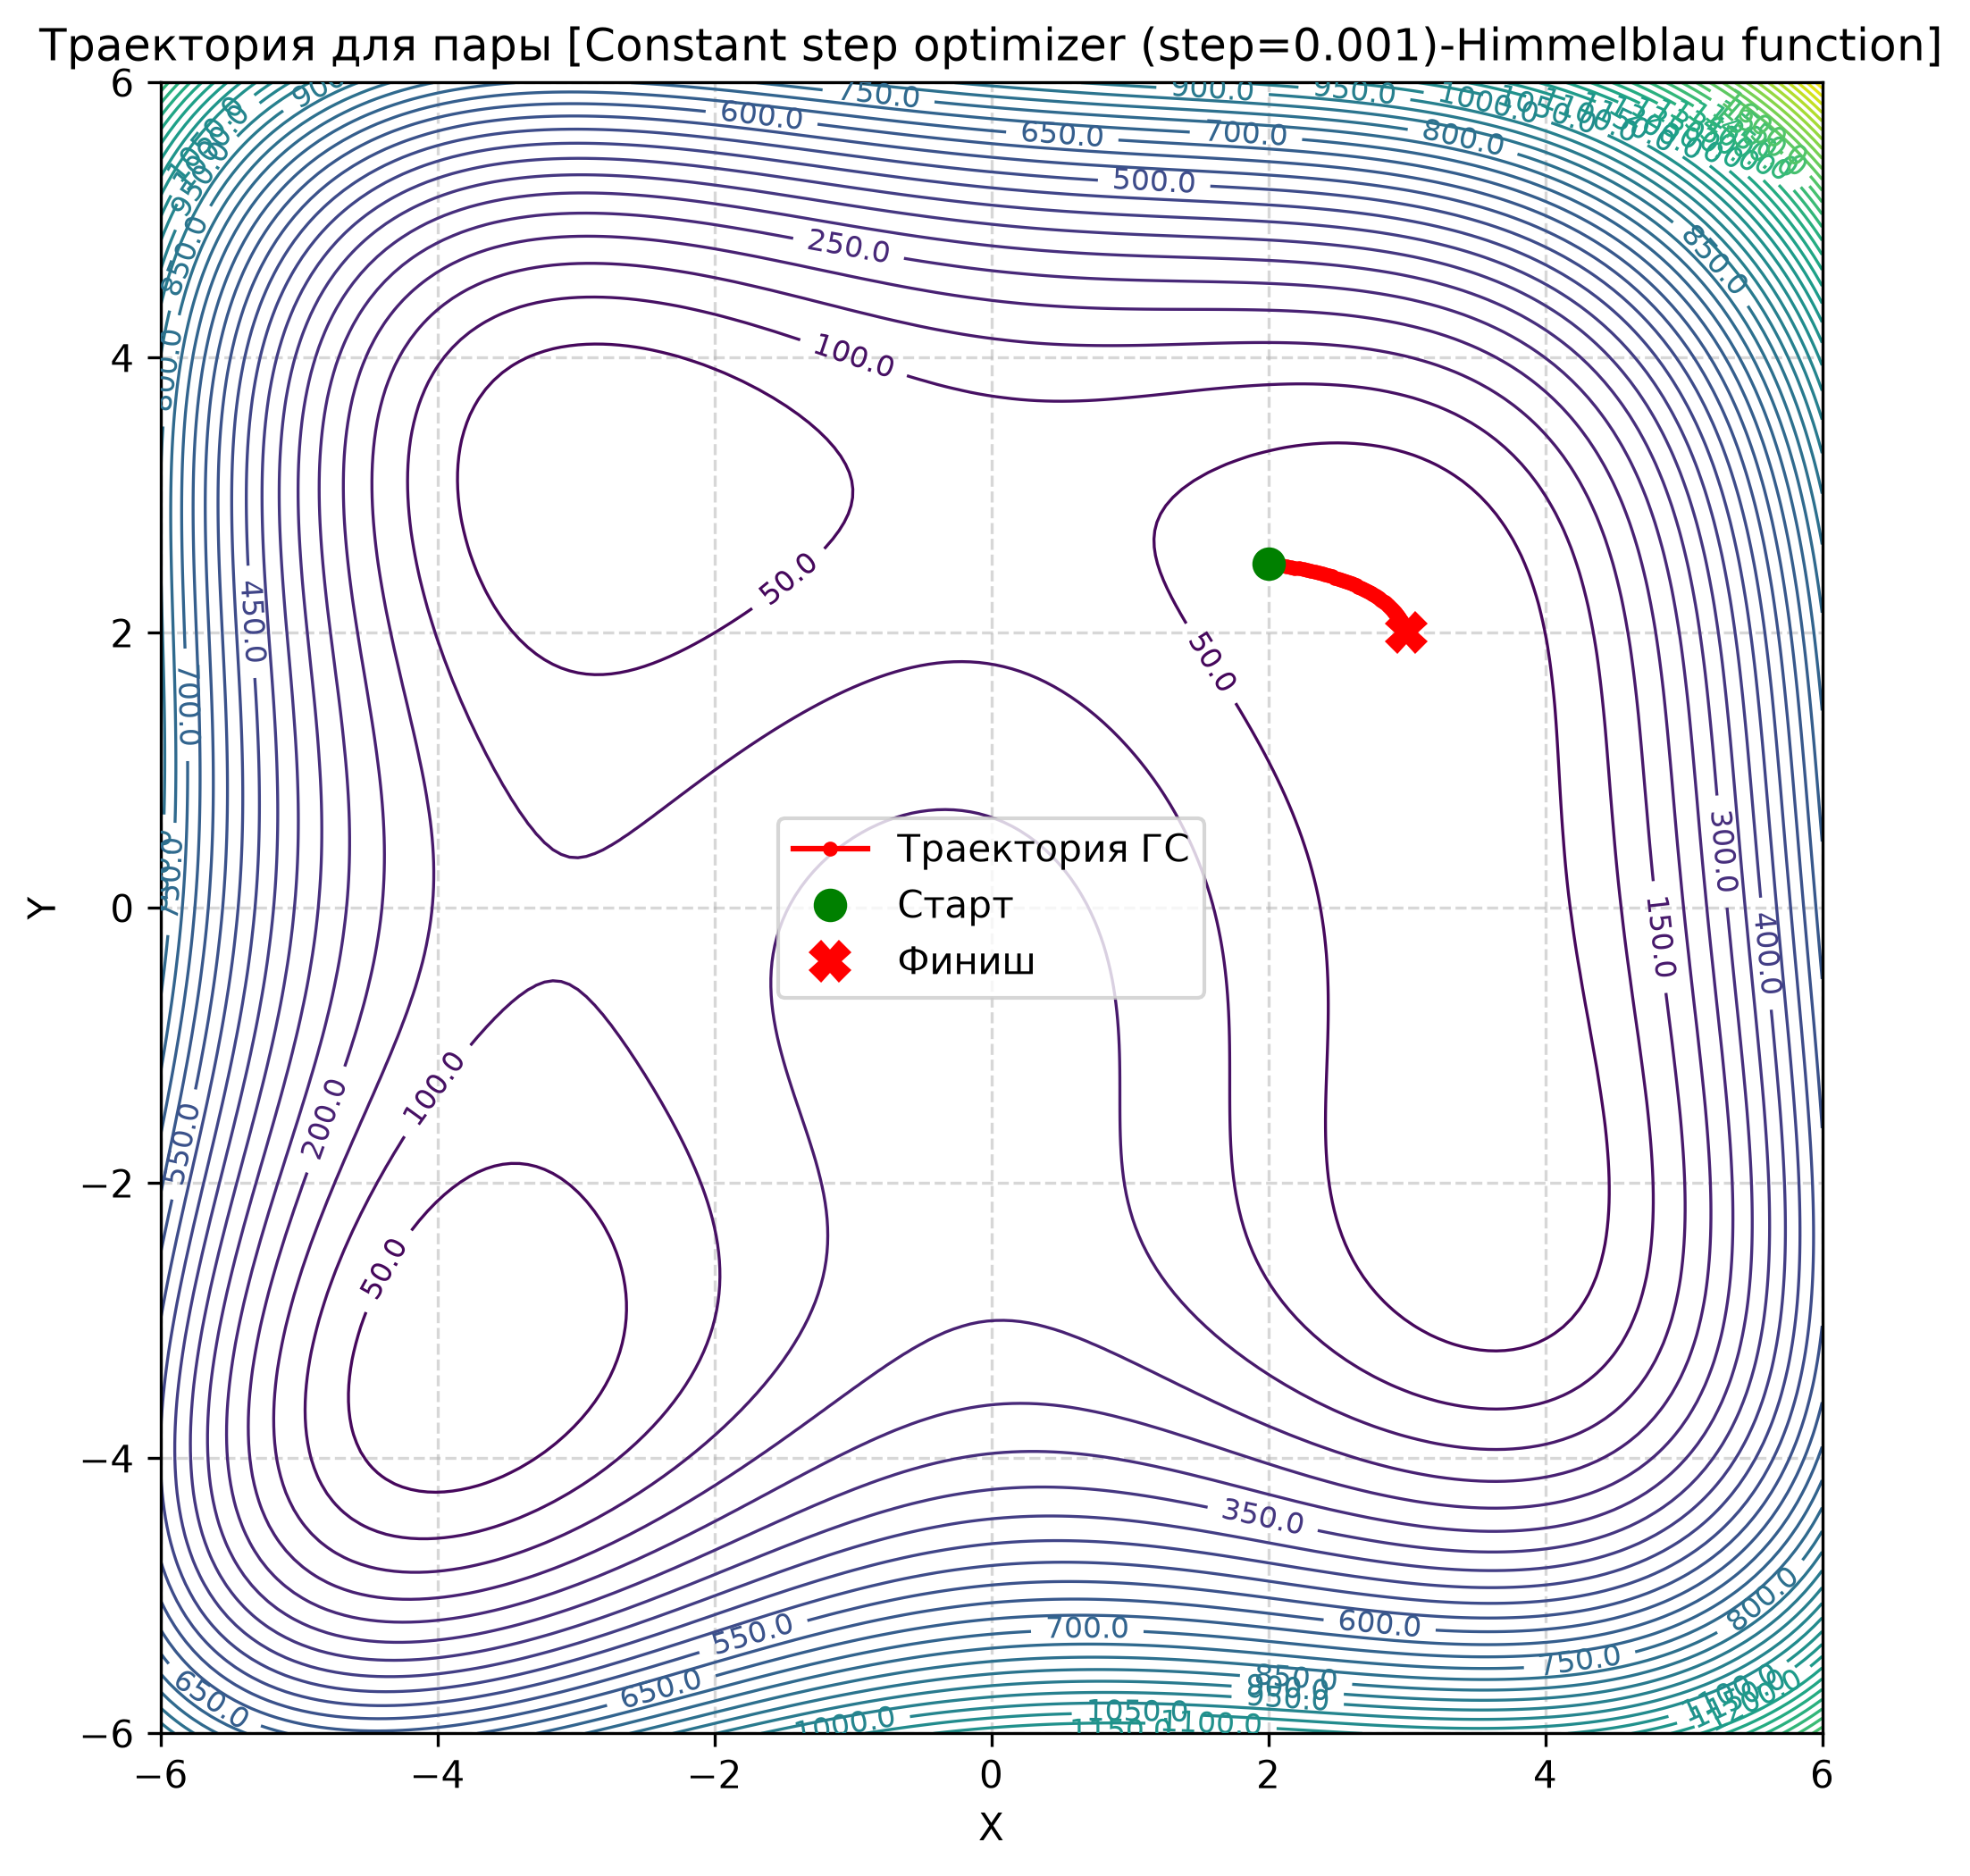
\includegraphics[width=0.7\linewidth]{plot_[Constant step optimizer (step=0.001)-Himmelblau function]__Trajectory.png}
    \caption{Траектория движения для функции Химмельблау.}
\end{figure}
\begin{figure}[H]
    \centering
    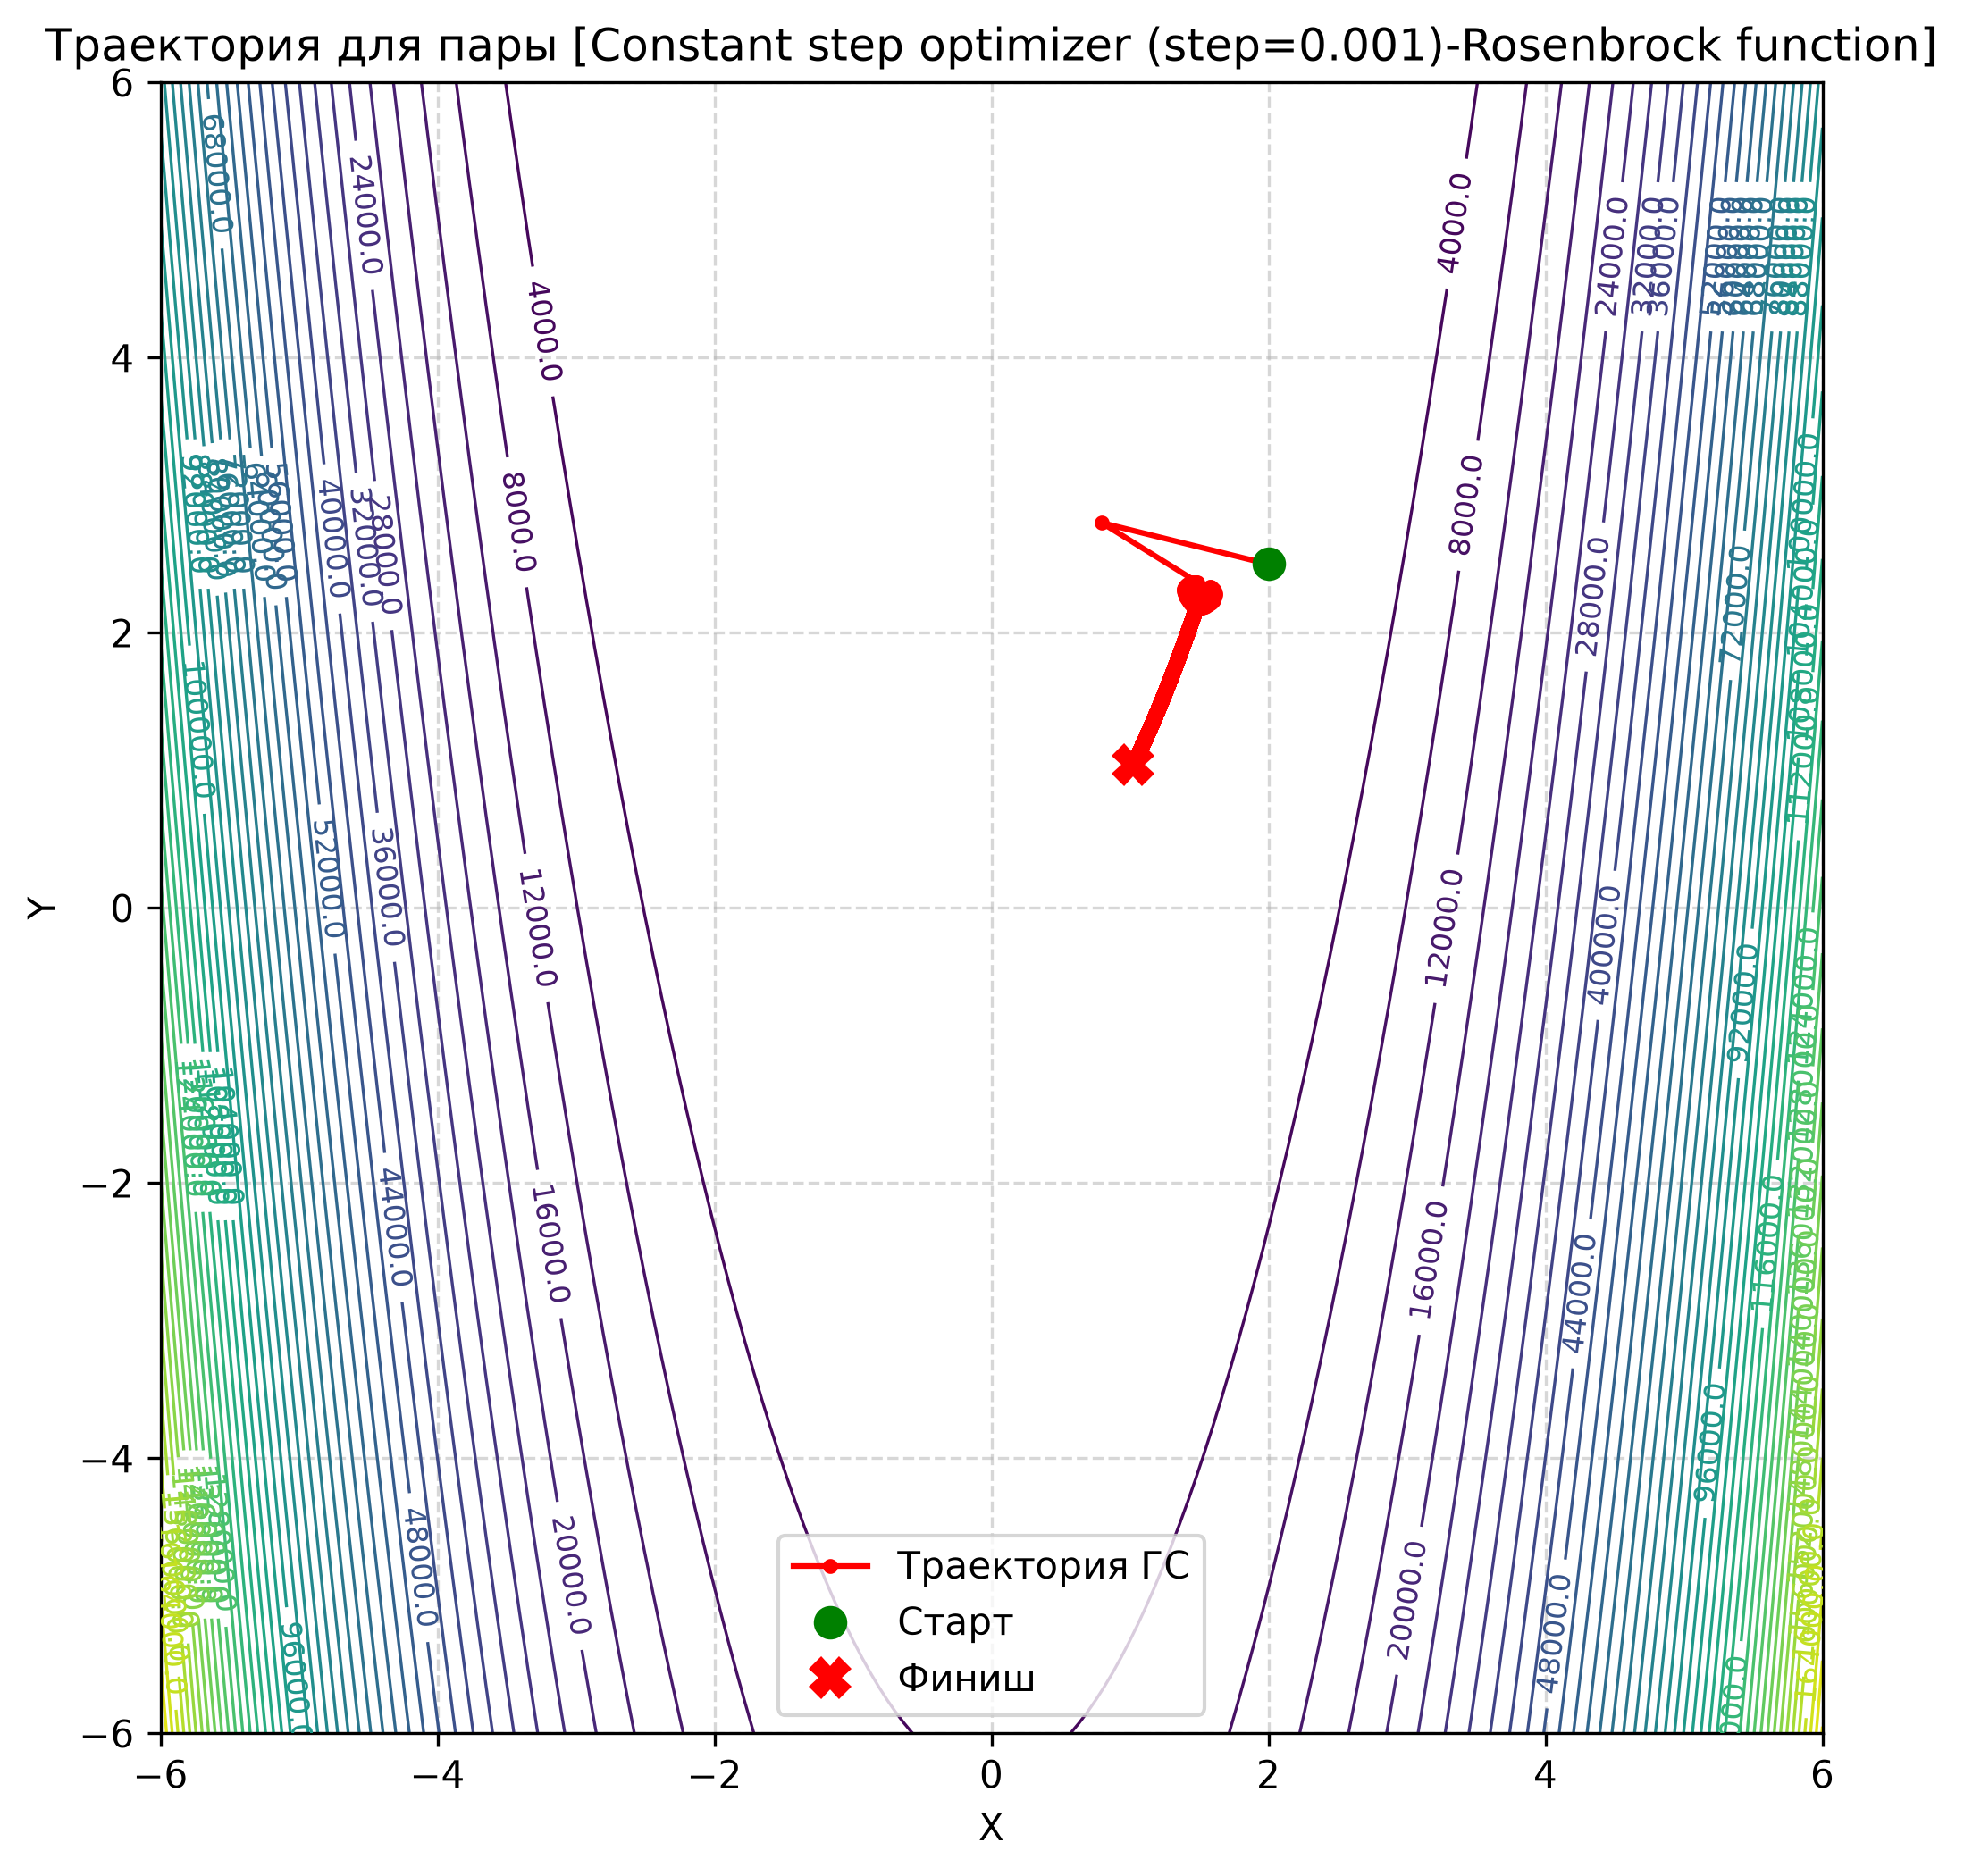
\includegraphics[width=0.7\linewidth]{plot_[Constant step optimizer (step=0.001)-Rosenbrock function]__Trajectory.png}
    \caption{Траектория движения для функции Розенброка.}
\end{figure}

\subsubsection{Сходимость методов с дроблением шага для квадратичных функций}

В рамках лабораторной работы была исследована зависимость количества итераций, вызовов функции и вызовов градиента от требуемой точности результата для квадратичных функций (начальная точка (2,2.5), лимит числа итераций 10000). Результаты приведены ниже в виде графиков.

\begin{figure}[H]
\centering
\subcaptionbox{Хорошая функция}{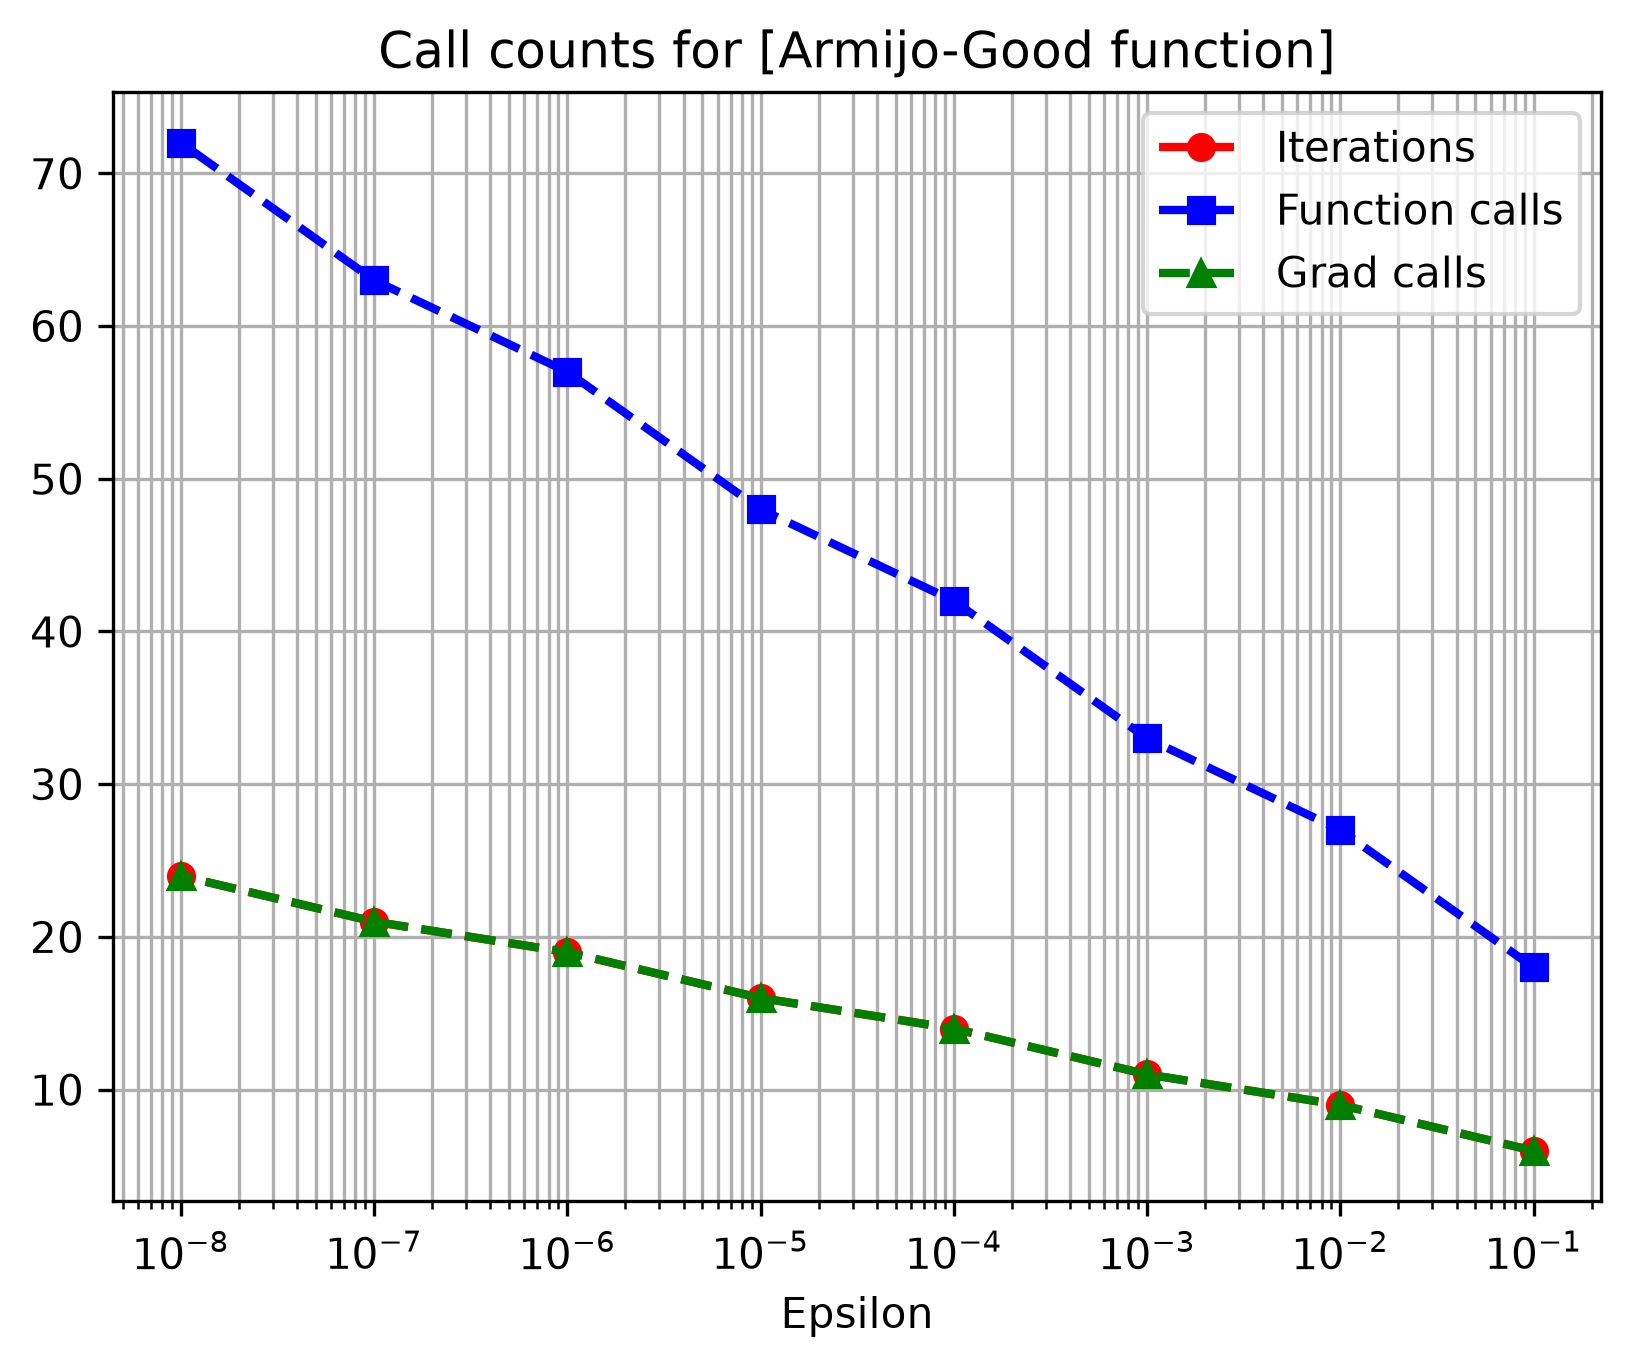
\includegraphics[width=0.475\textwidth]{task4_[Armijo-Good function]_plot.png}}%
%\hfill % <-- Seperation
\subcaptionbox{Плохая функция}{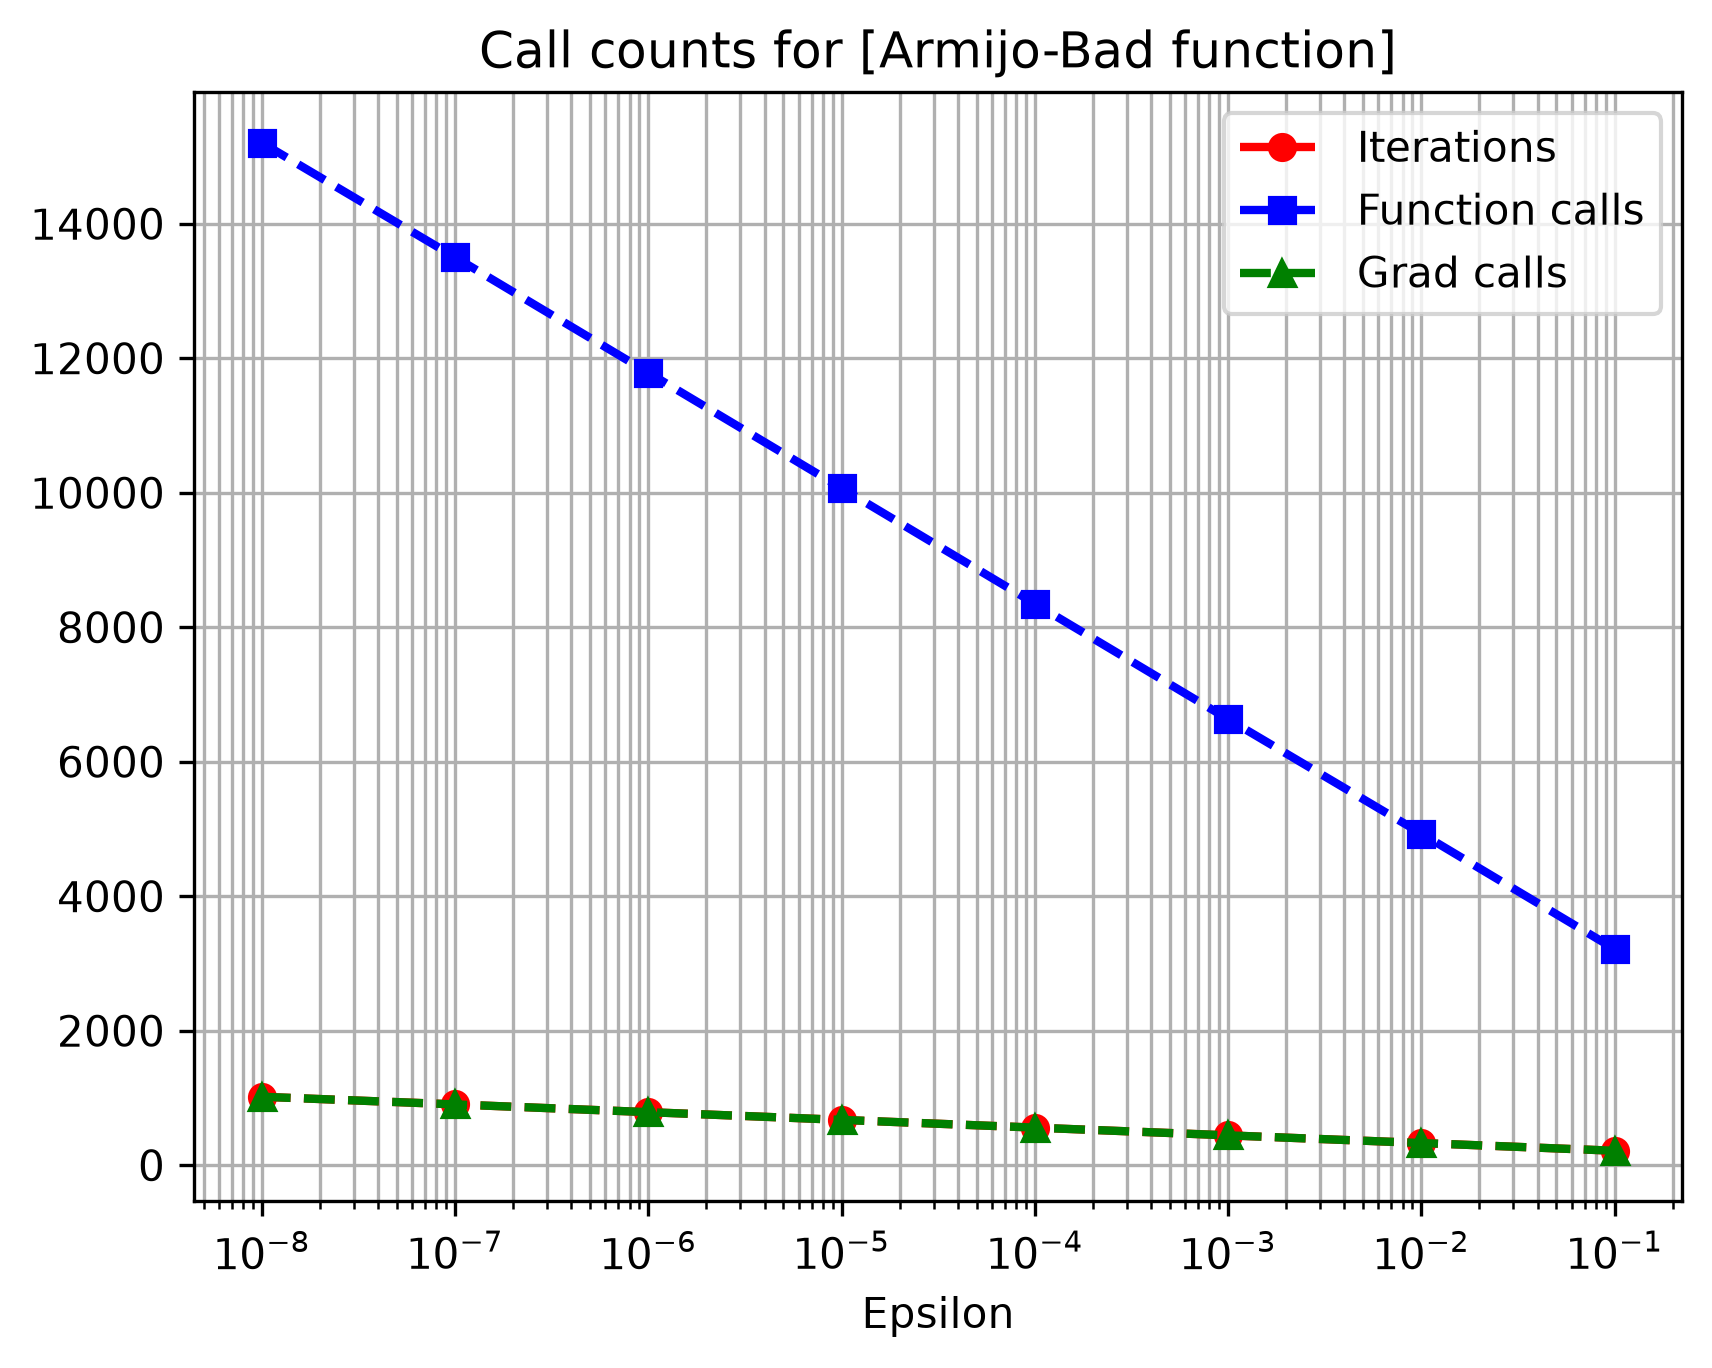
\includegraphics[width=0.5\textwidth]{task4_[Armijo-Bad function]_plot.png}}%
\caption{Условия Армихо для квадратичных функций.}
\end{figure}

\begin{figure}[H]
\centering
\subcaptionbox{Хорошая функция}{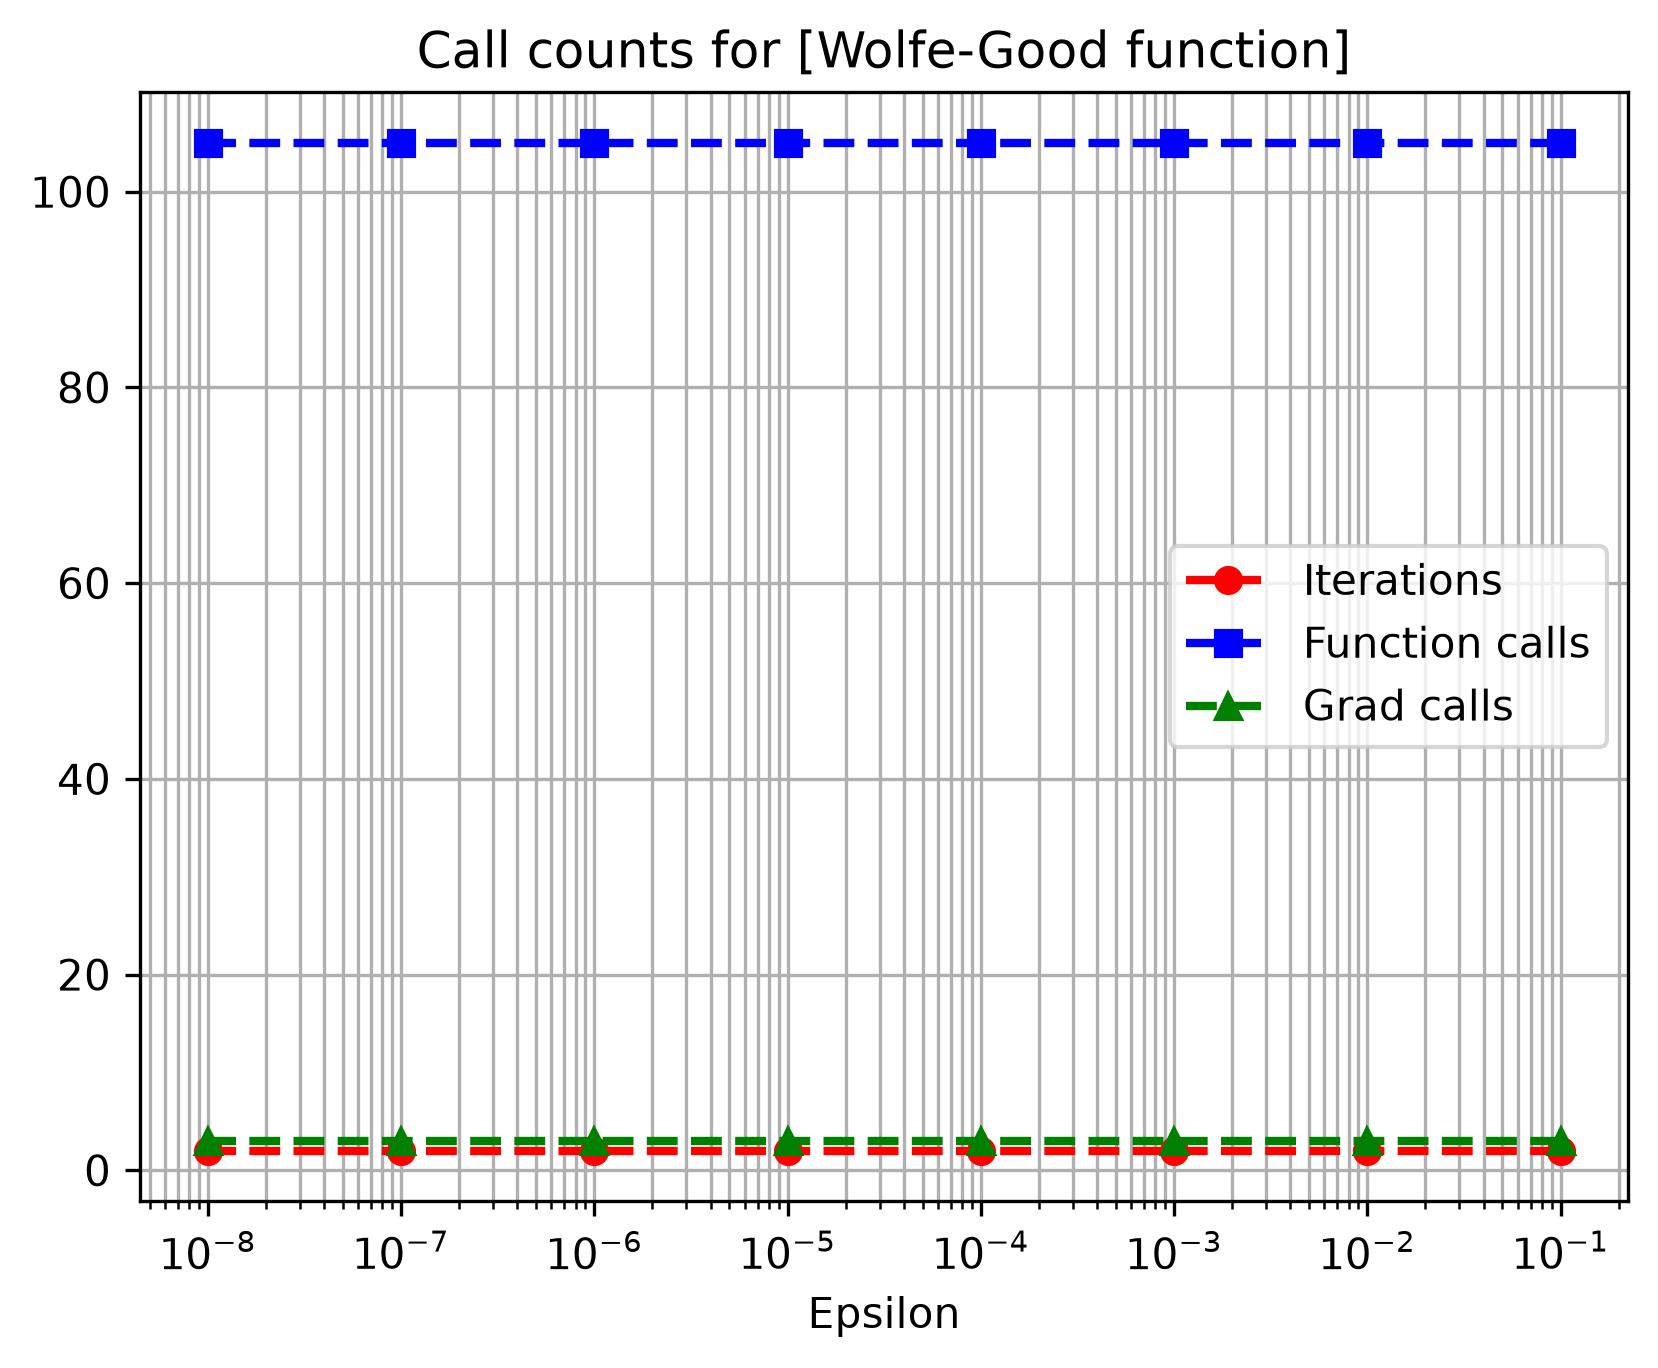
\includegraphics[width=0.49\textwidth]{task4_[Wolfe-Good function]_plot.png}}%
%\hfill % <-- Seperation
\subcaptionbox{Плохая функция}{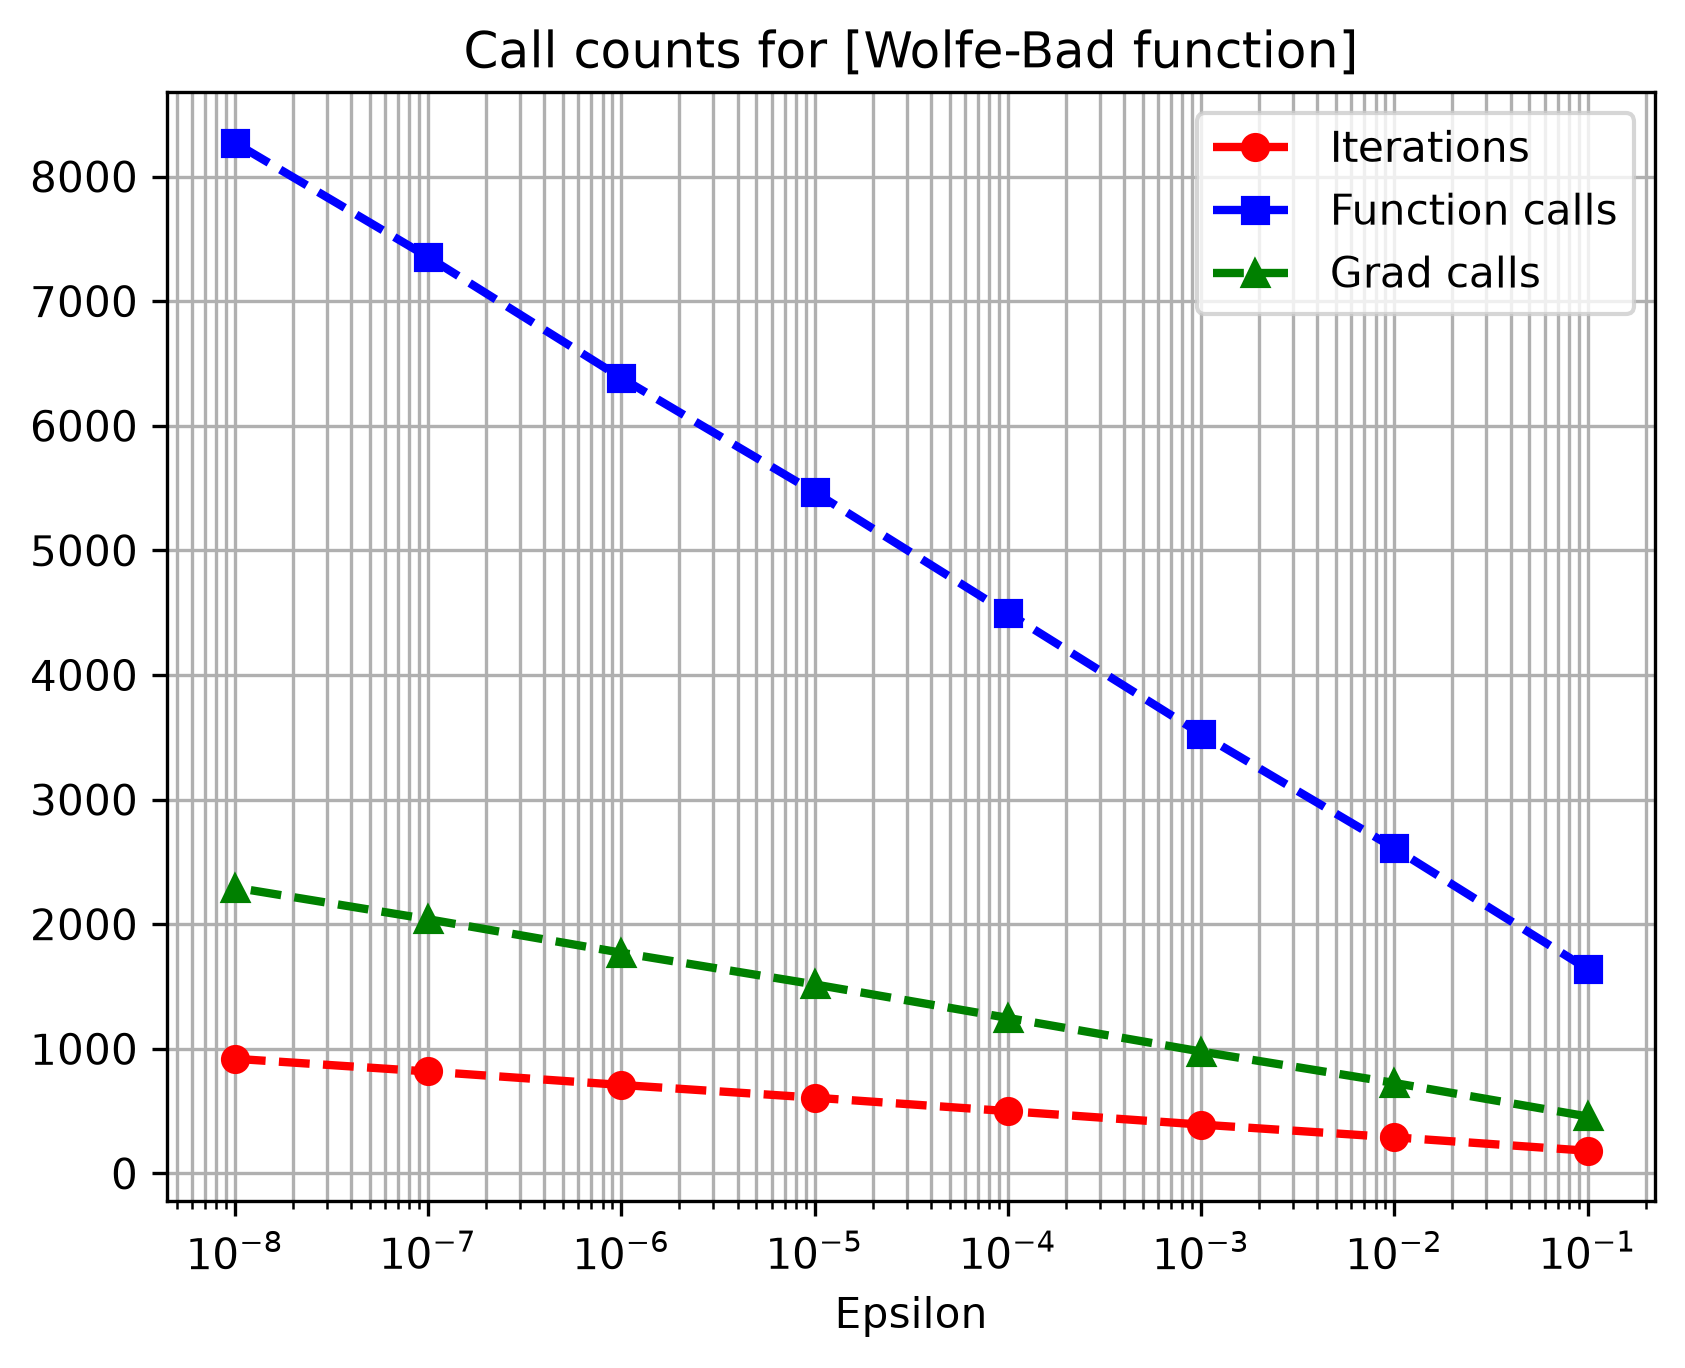
\includegraphics[width=0.5\textwidth]{task4_[Wolfe-Bad function]_plot.png}}%
\caption{Сильные условия Вольфе для квадратичных функций.}
\end{figure}

Заметим, что, хотя число итераций относительно невелико, число вызовов функций заметно превышает число итераций и число вызовов градиента. В случае условий Армихо число вызовов градиента строго равно числу итераций. Это логично, ведь для проверки условий Армихо не требуется знаний о градиенте функции. Настолько же логичным кажется то, что число вызовов градиента в случае сильных условий Вольфе больше, чем число итераций, ведь проверка условий требует знаний о градиенте функции. Заметим, наконец, что число итераций, вызовов функции и вызовов градиента зависят от точности логарифмически. Это вызвано линейной скоростью сходимости методов, которая, в свою очередь, обусловлена сильной выпуклостью приведенных квадратичных функций.

Следующие четыре графика траекторий движения демонстрируют работу алгоритма для квадратичных функций ($\varepsilon = 10^{-5})$:

\begin{figure}[H]
\centering
\subcaptionbox{Хорошая функция}{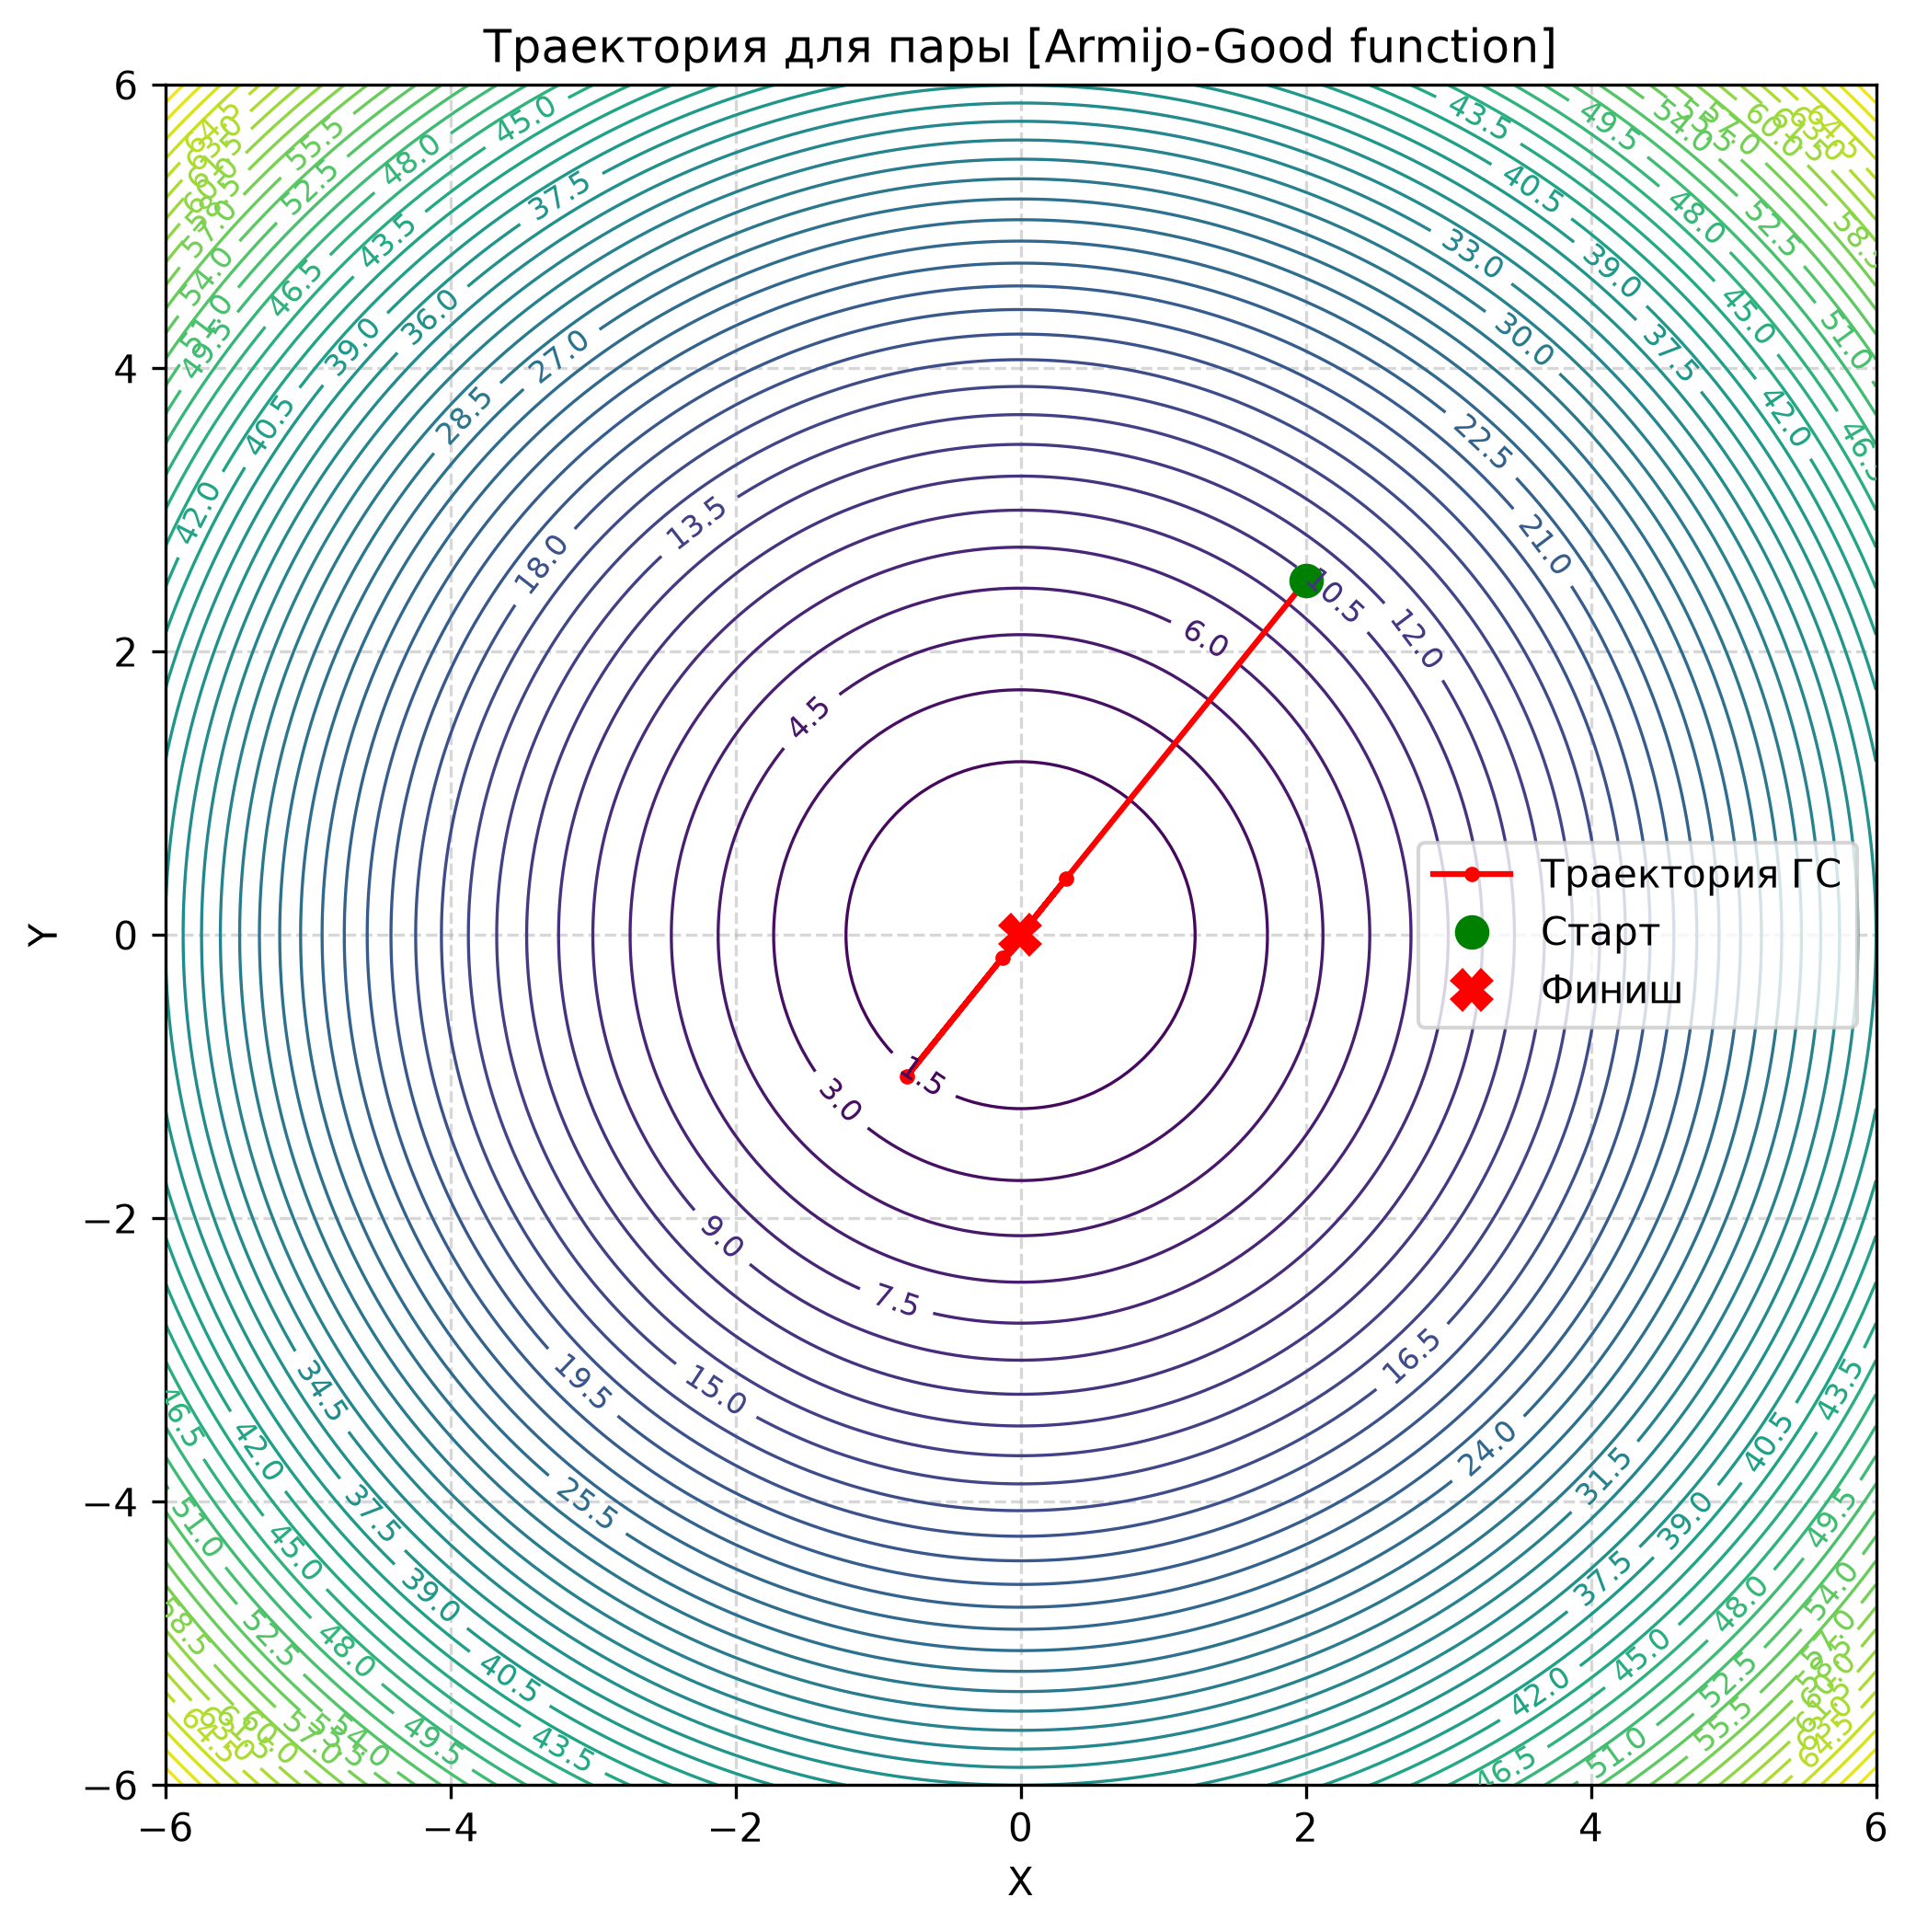
\includegraphics[width=0.49\textwidth]{plot_[Armijo-Good function]__Trajectory.png}}%
%\hfill % <-- Seperation
\subcaptionbox{Плохая функция}{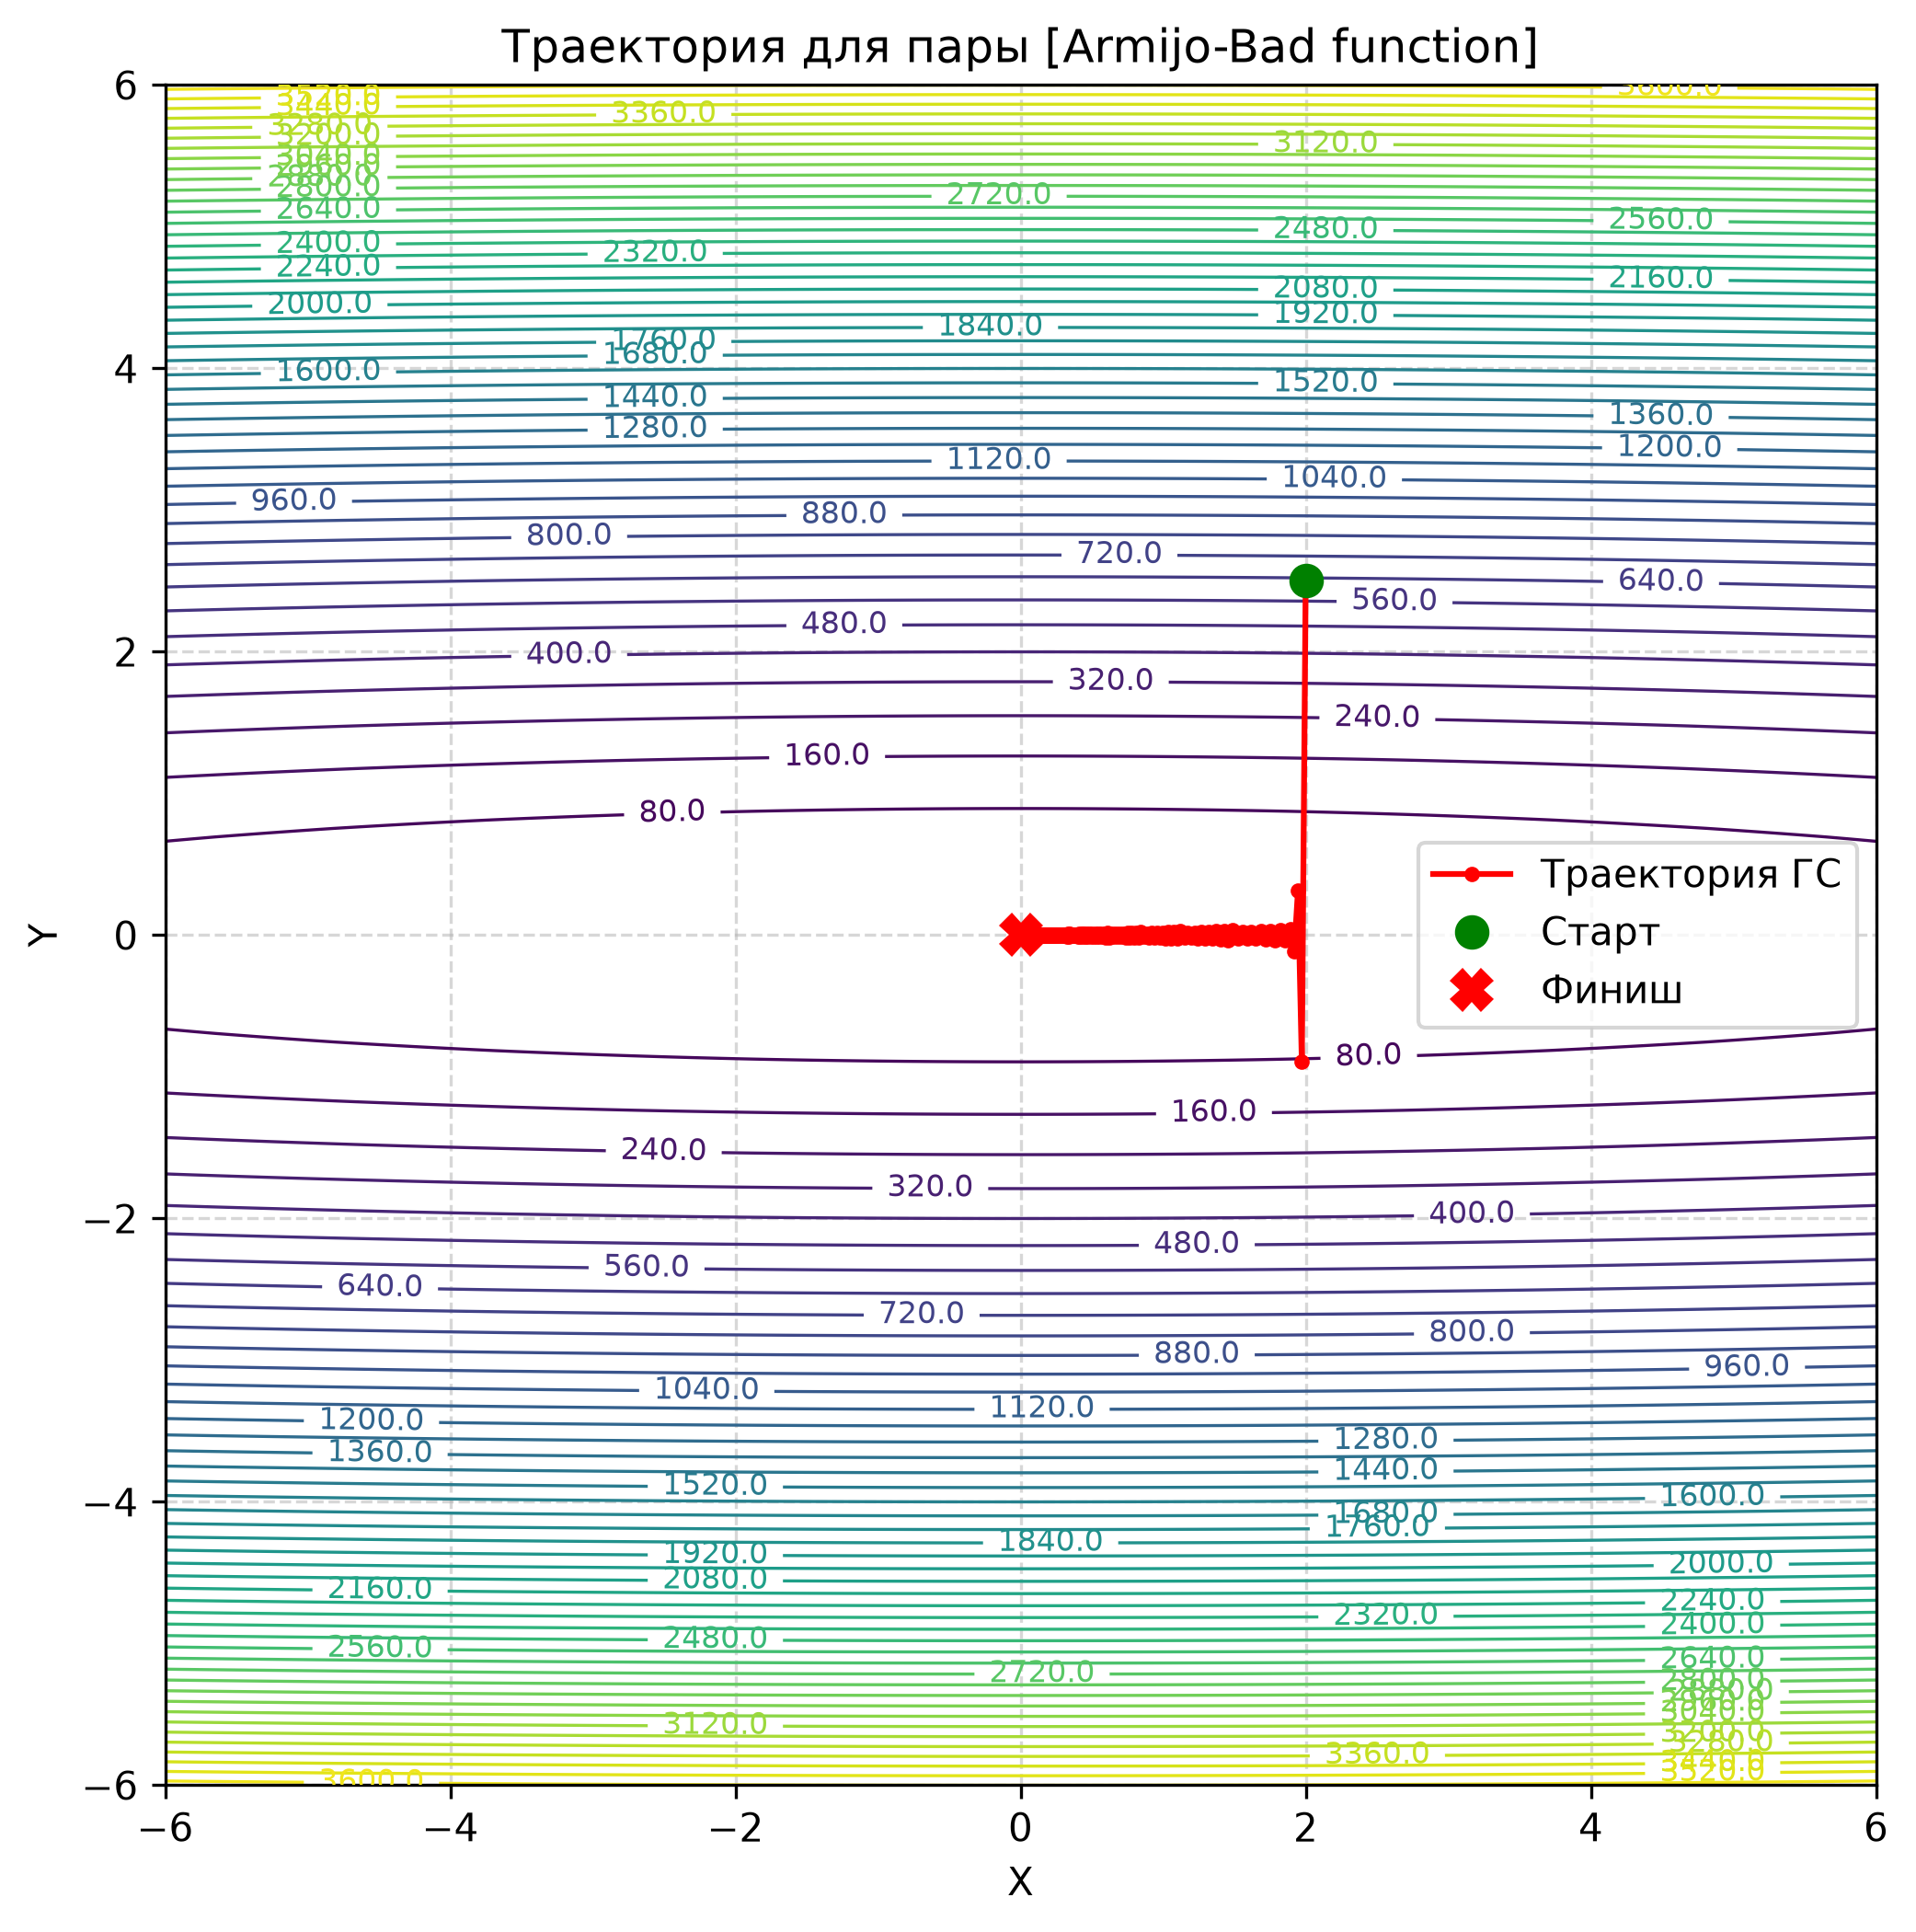
\includegraphics[width=0.5\textwidth]{plot_[Armijo-Bad function]__Trajectory.png}}%
\caption{Условия Армихо для квадратичных функций. Траектория алгоритма.}
\end{figure}

\begin{figure}[H]
\centering
\subcaptionbox{Хорошая функция}{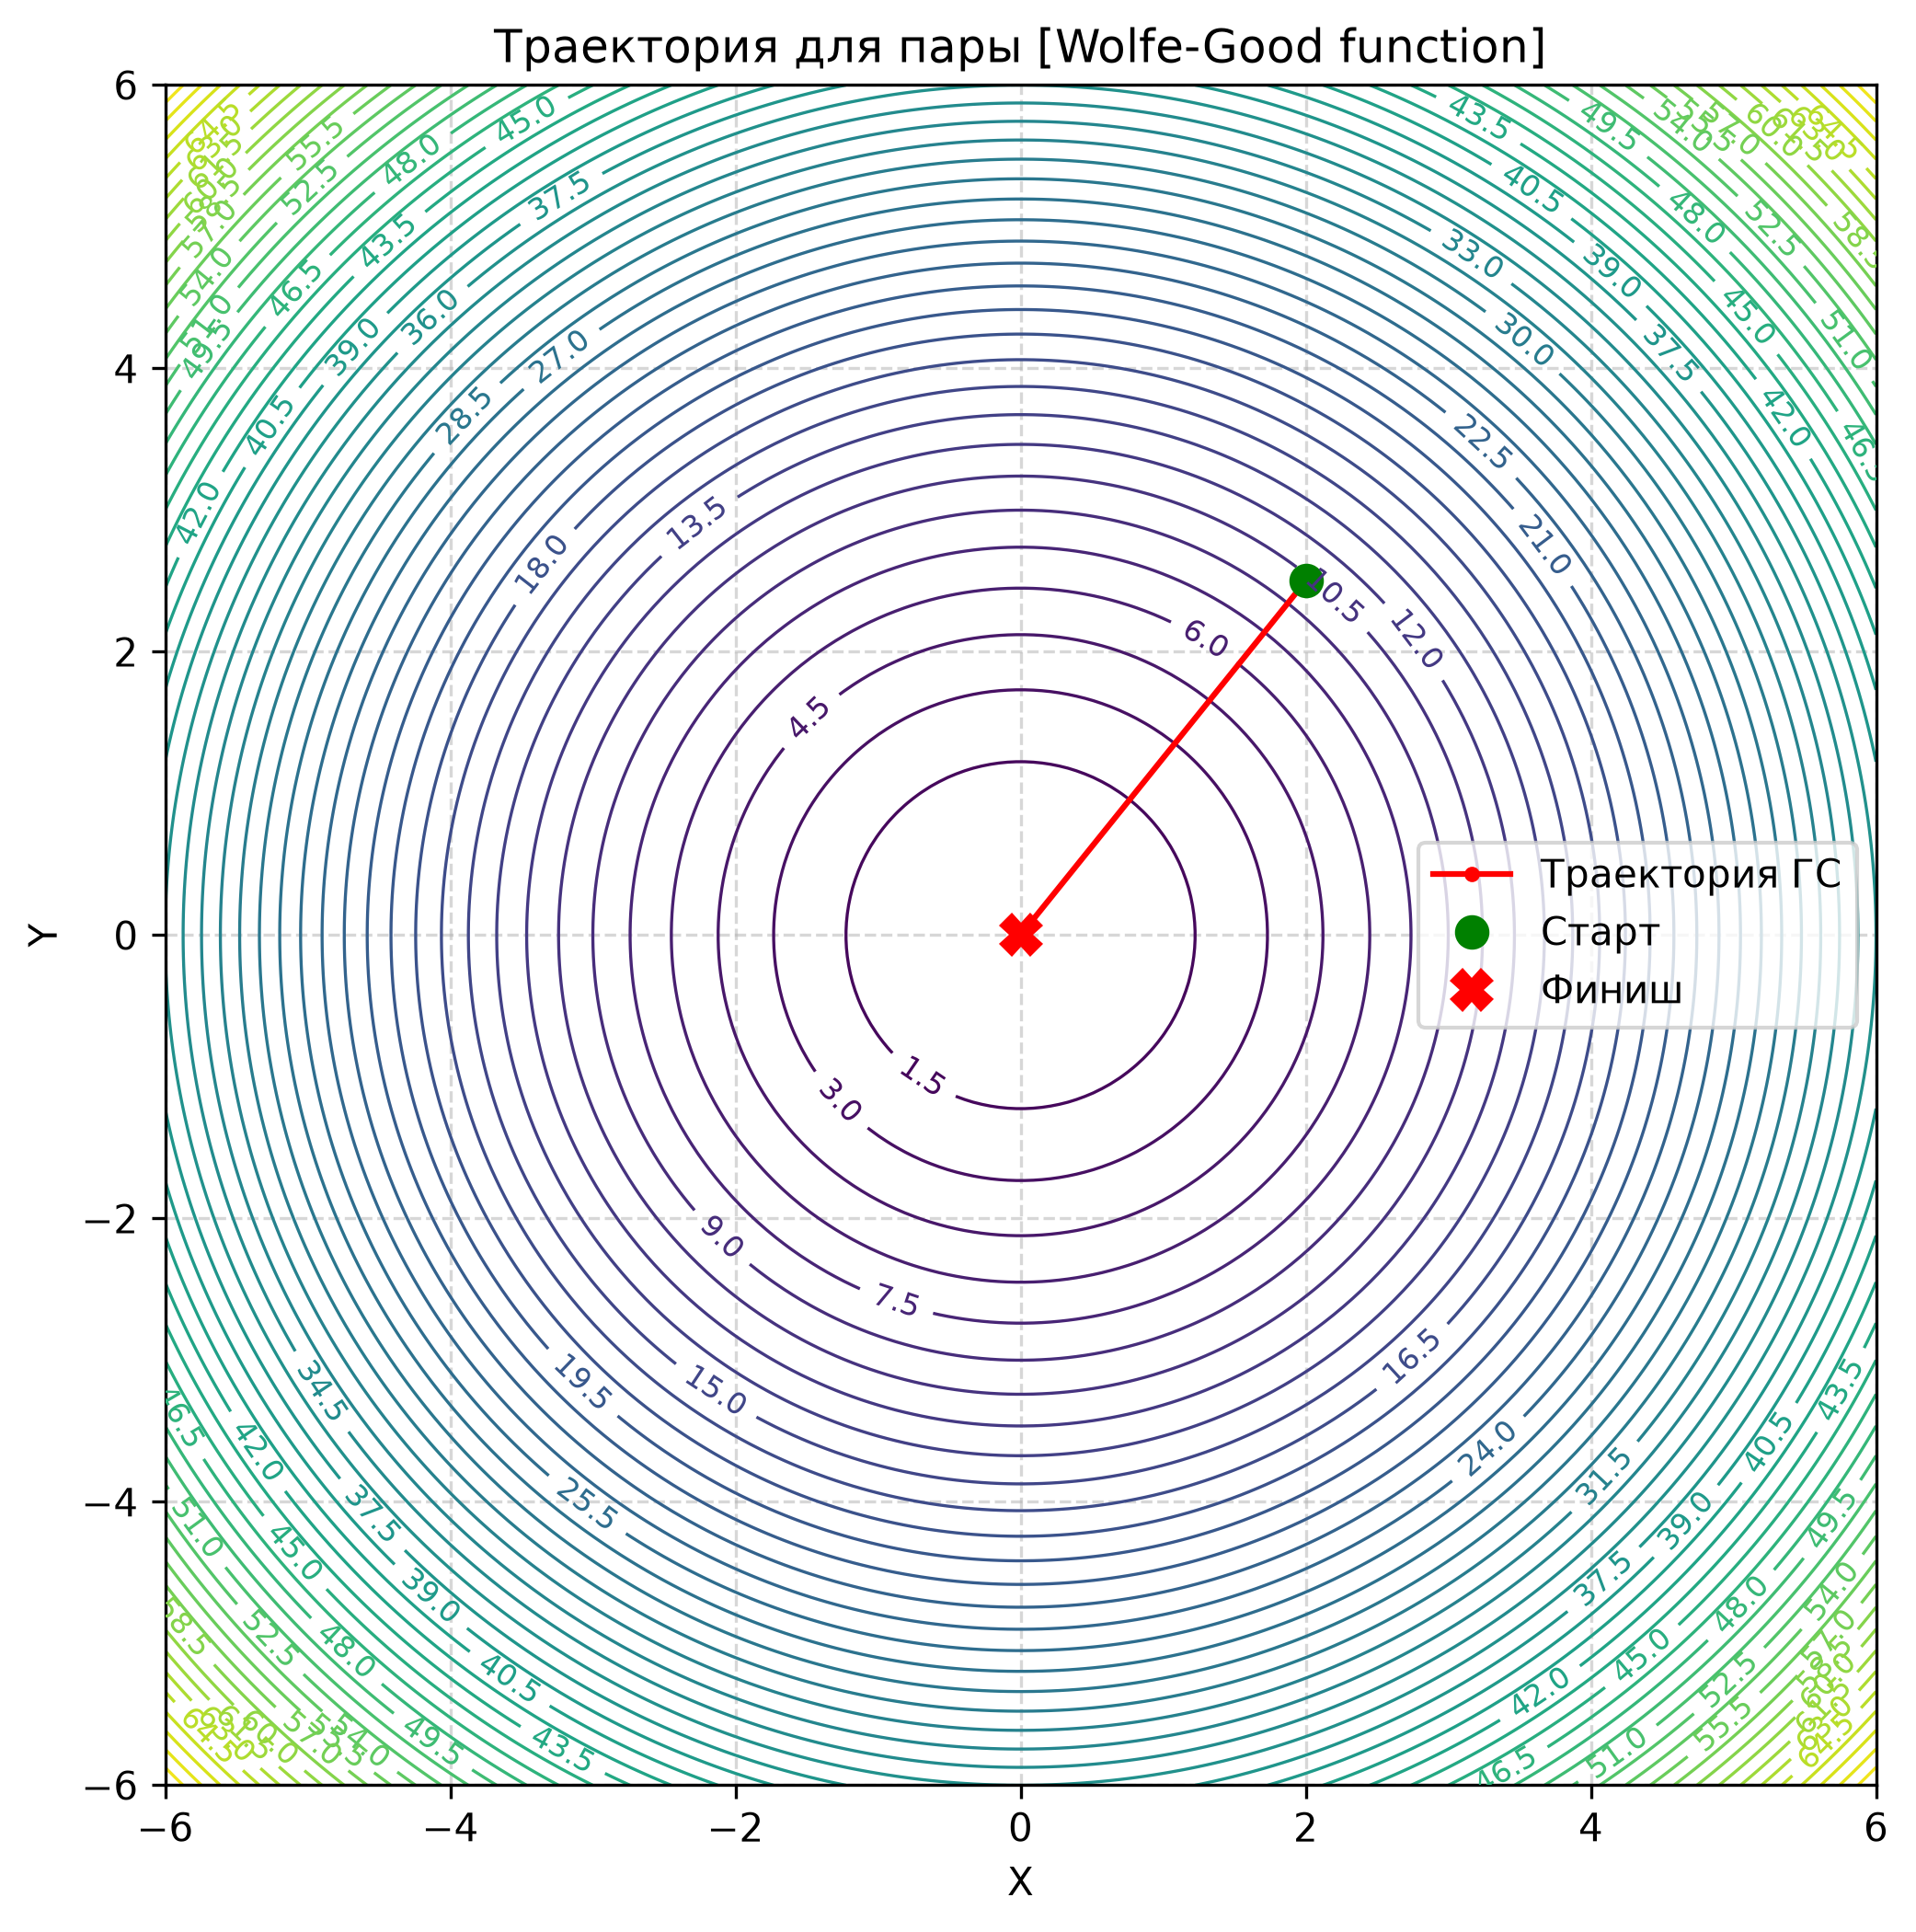
\includegraphics[width=0.49\textwidth]{plot_[Wolfe-Good function]__Trajectory.png}}%
%\hfill % <-- Seperation
\subcaptionbox{Плохая функция}{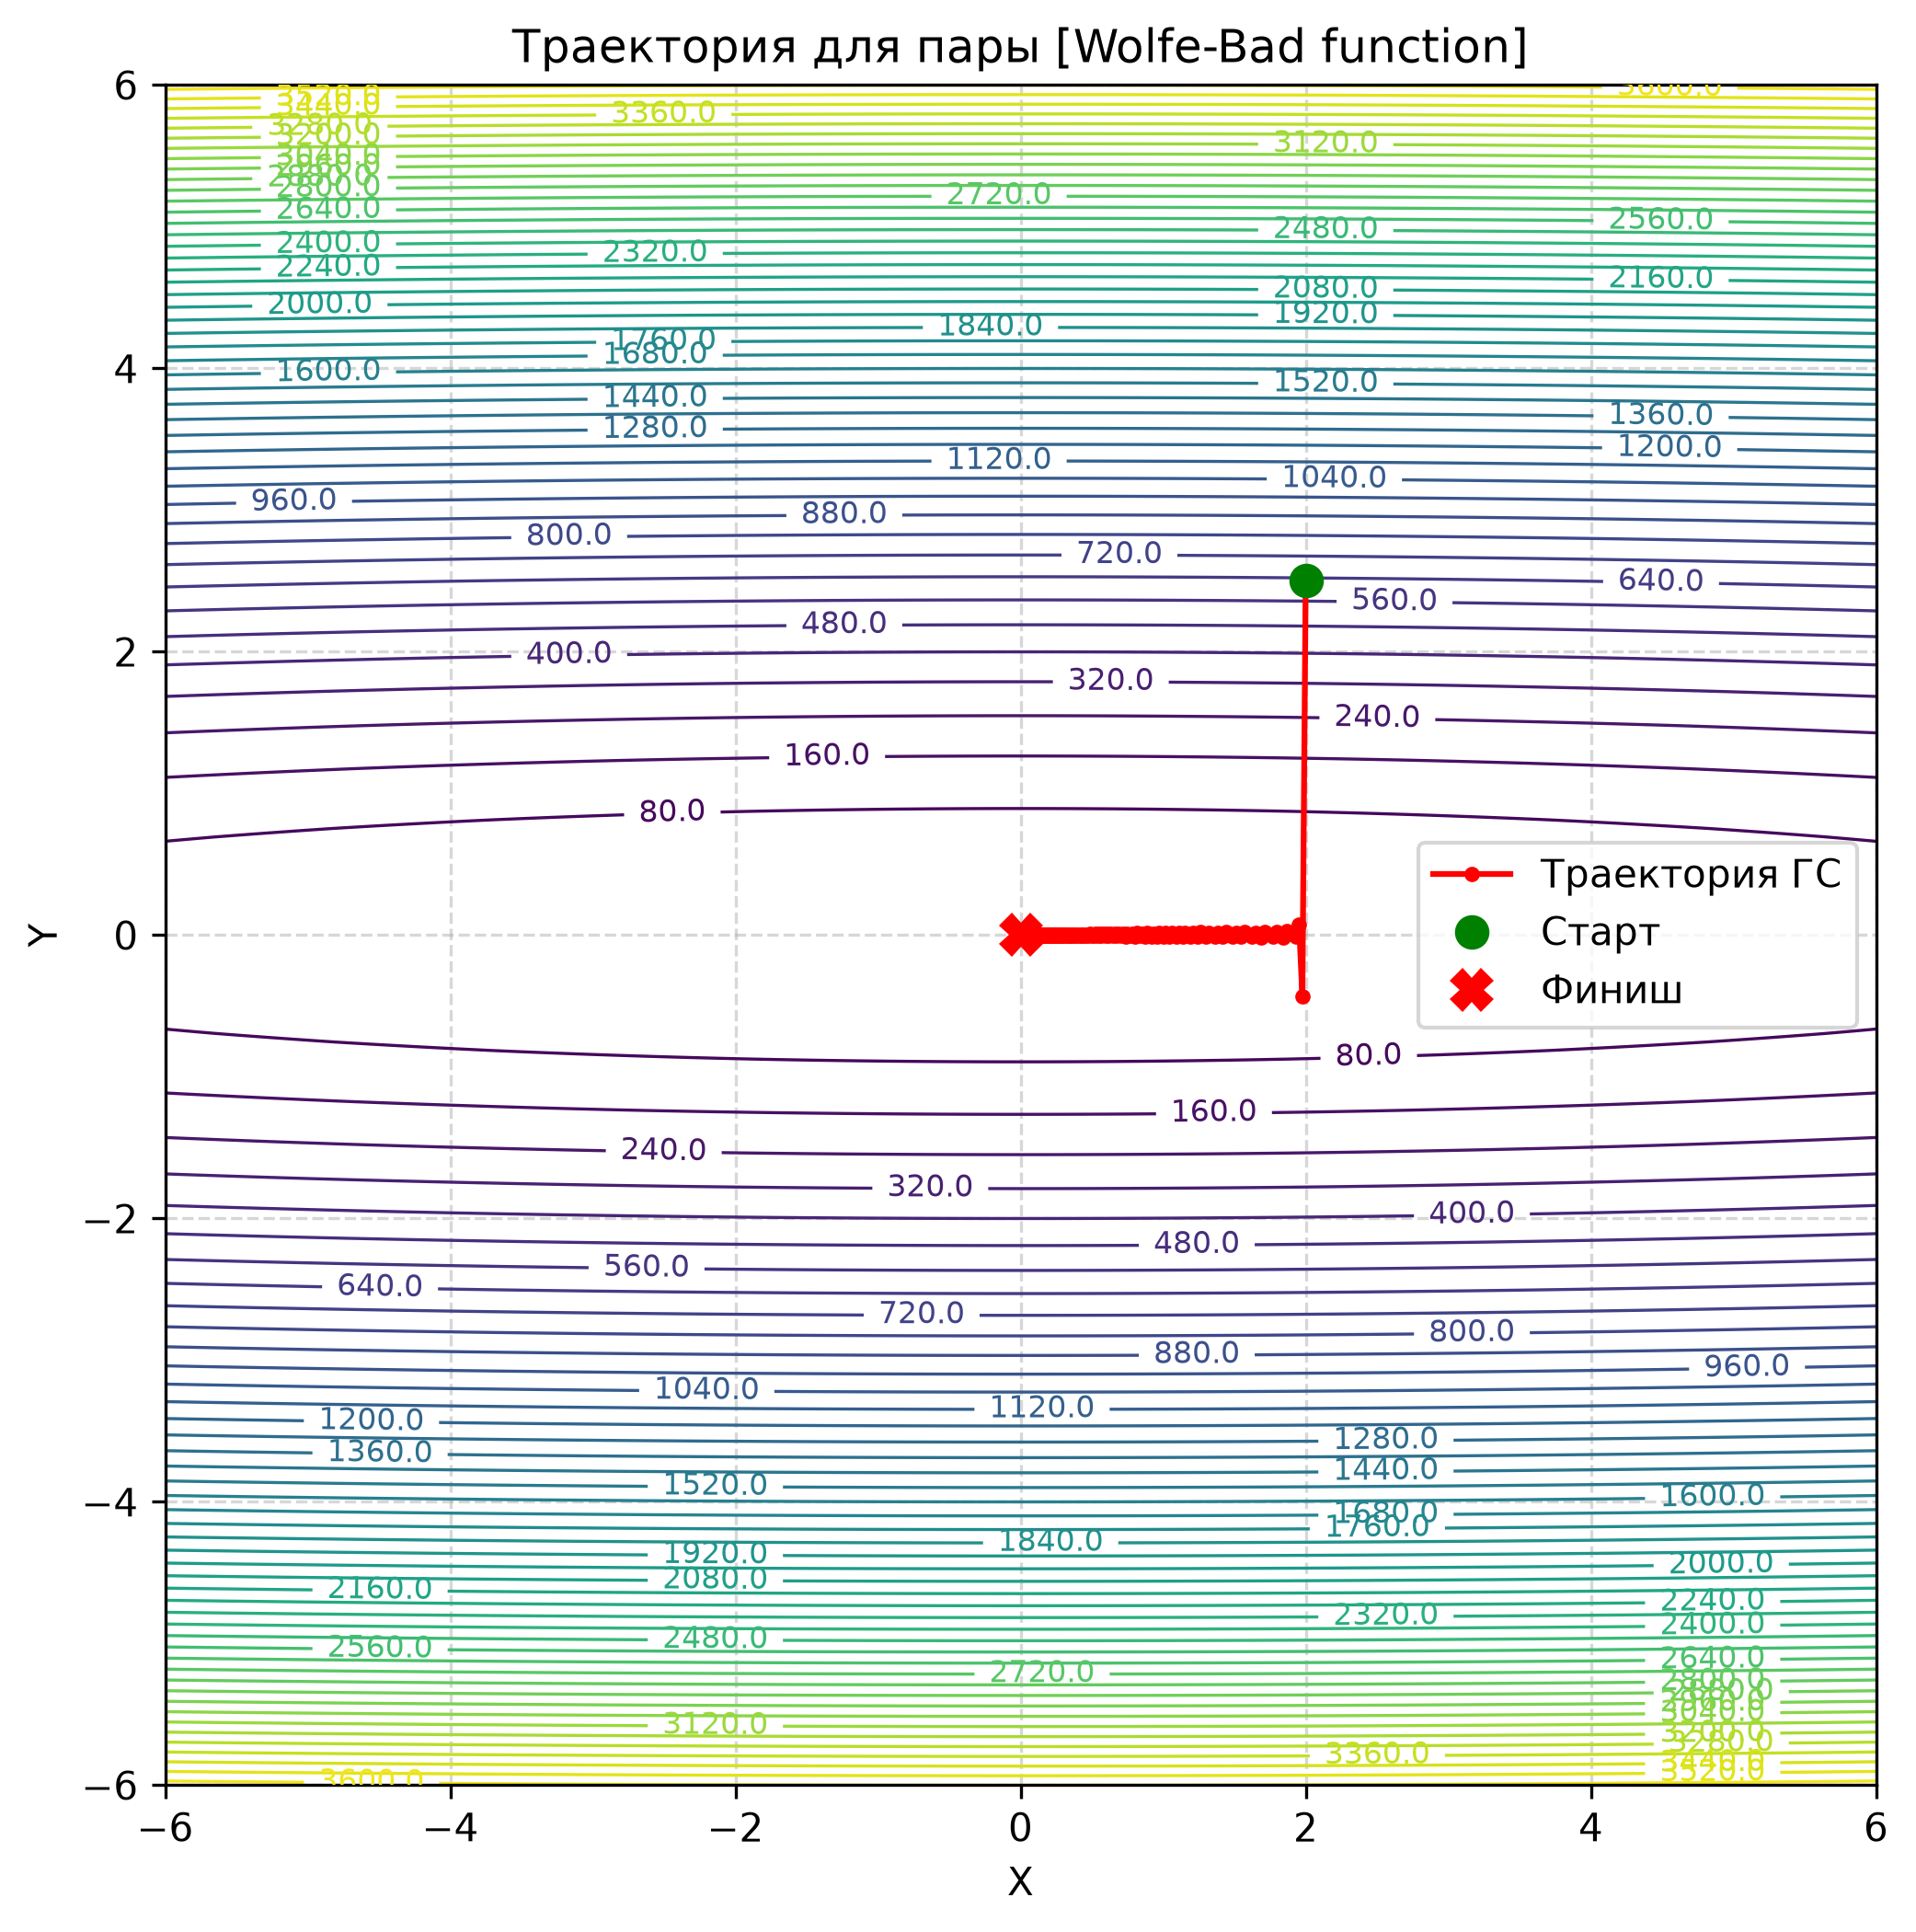
\includegraphics[width=0.5\textwidth]{plot_[Wolfe-Bad function]__Trajectory.png}}%
\caption{Сильные условия Армихо для квадратичных функций. Траектория алгоритма.}
\end{figure}

\subsubsection{Сходимость методов с дроблением шага для сложных функций}

В рамках лабораторной работы было исследовано поведение методов с дроблением шага для сложных функций в зависимости от начального положения. Использованные точки: (2,2.5), (3,3), (4,1), (0,2), (-1,3).

Заметим, что в случае функций Химмельблау и Розенброка все алгоритмы сходились к искомому минимуму функции, хотя, например, в случае функции Химмельблау, алгоритмы в зависимости от начального положения могли сойтись к разным точкам минимума:

\begin{figure}[H]
\centering
\subcaptionbox{Нач. точка (0,2)}{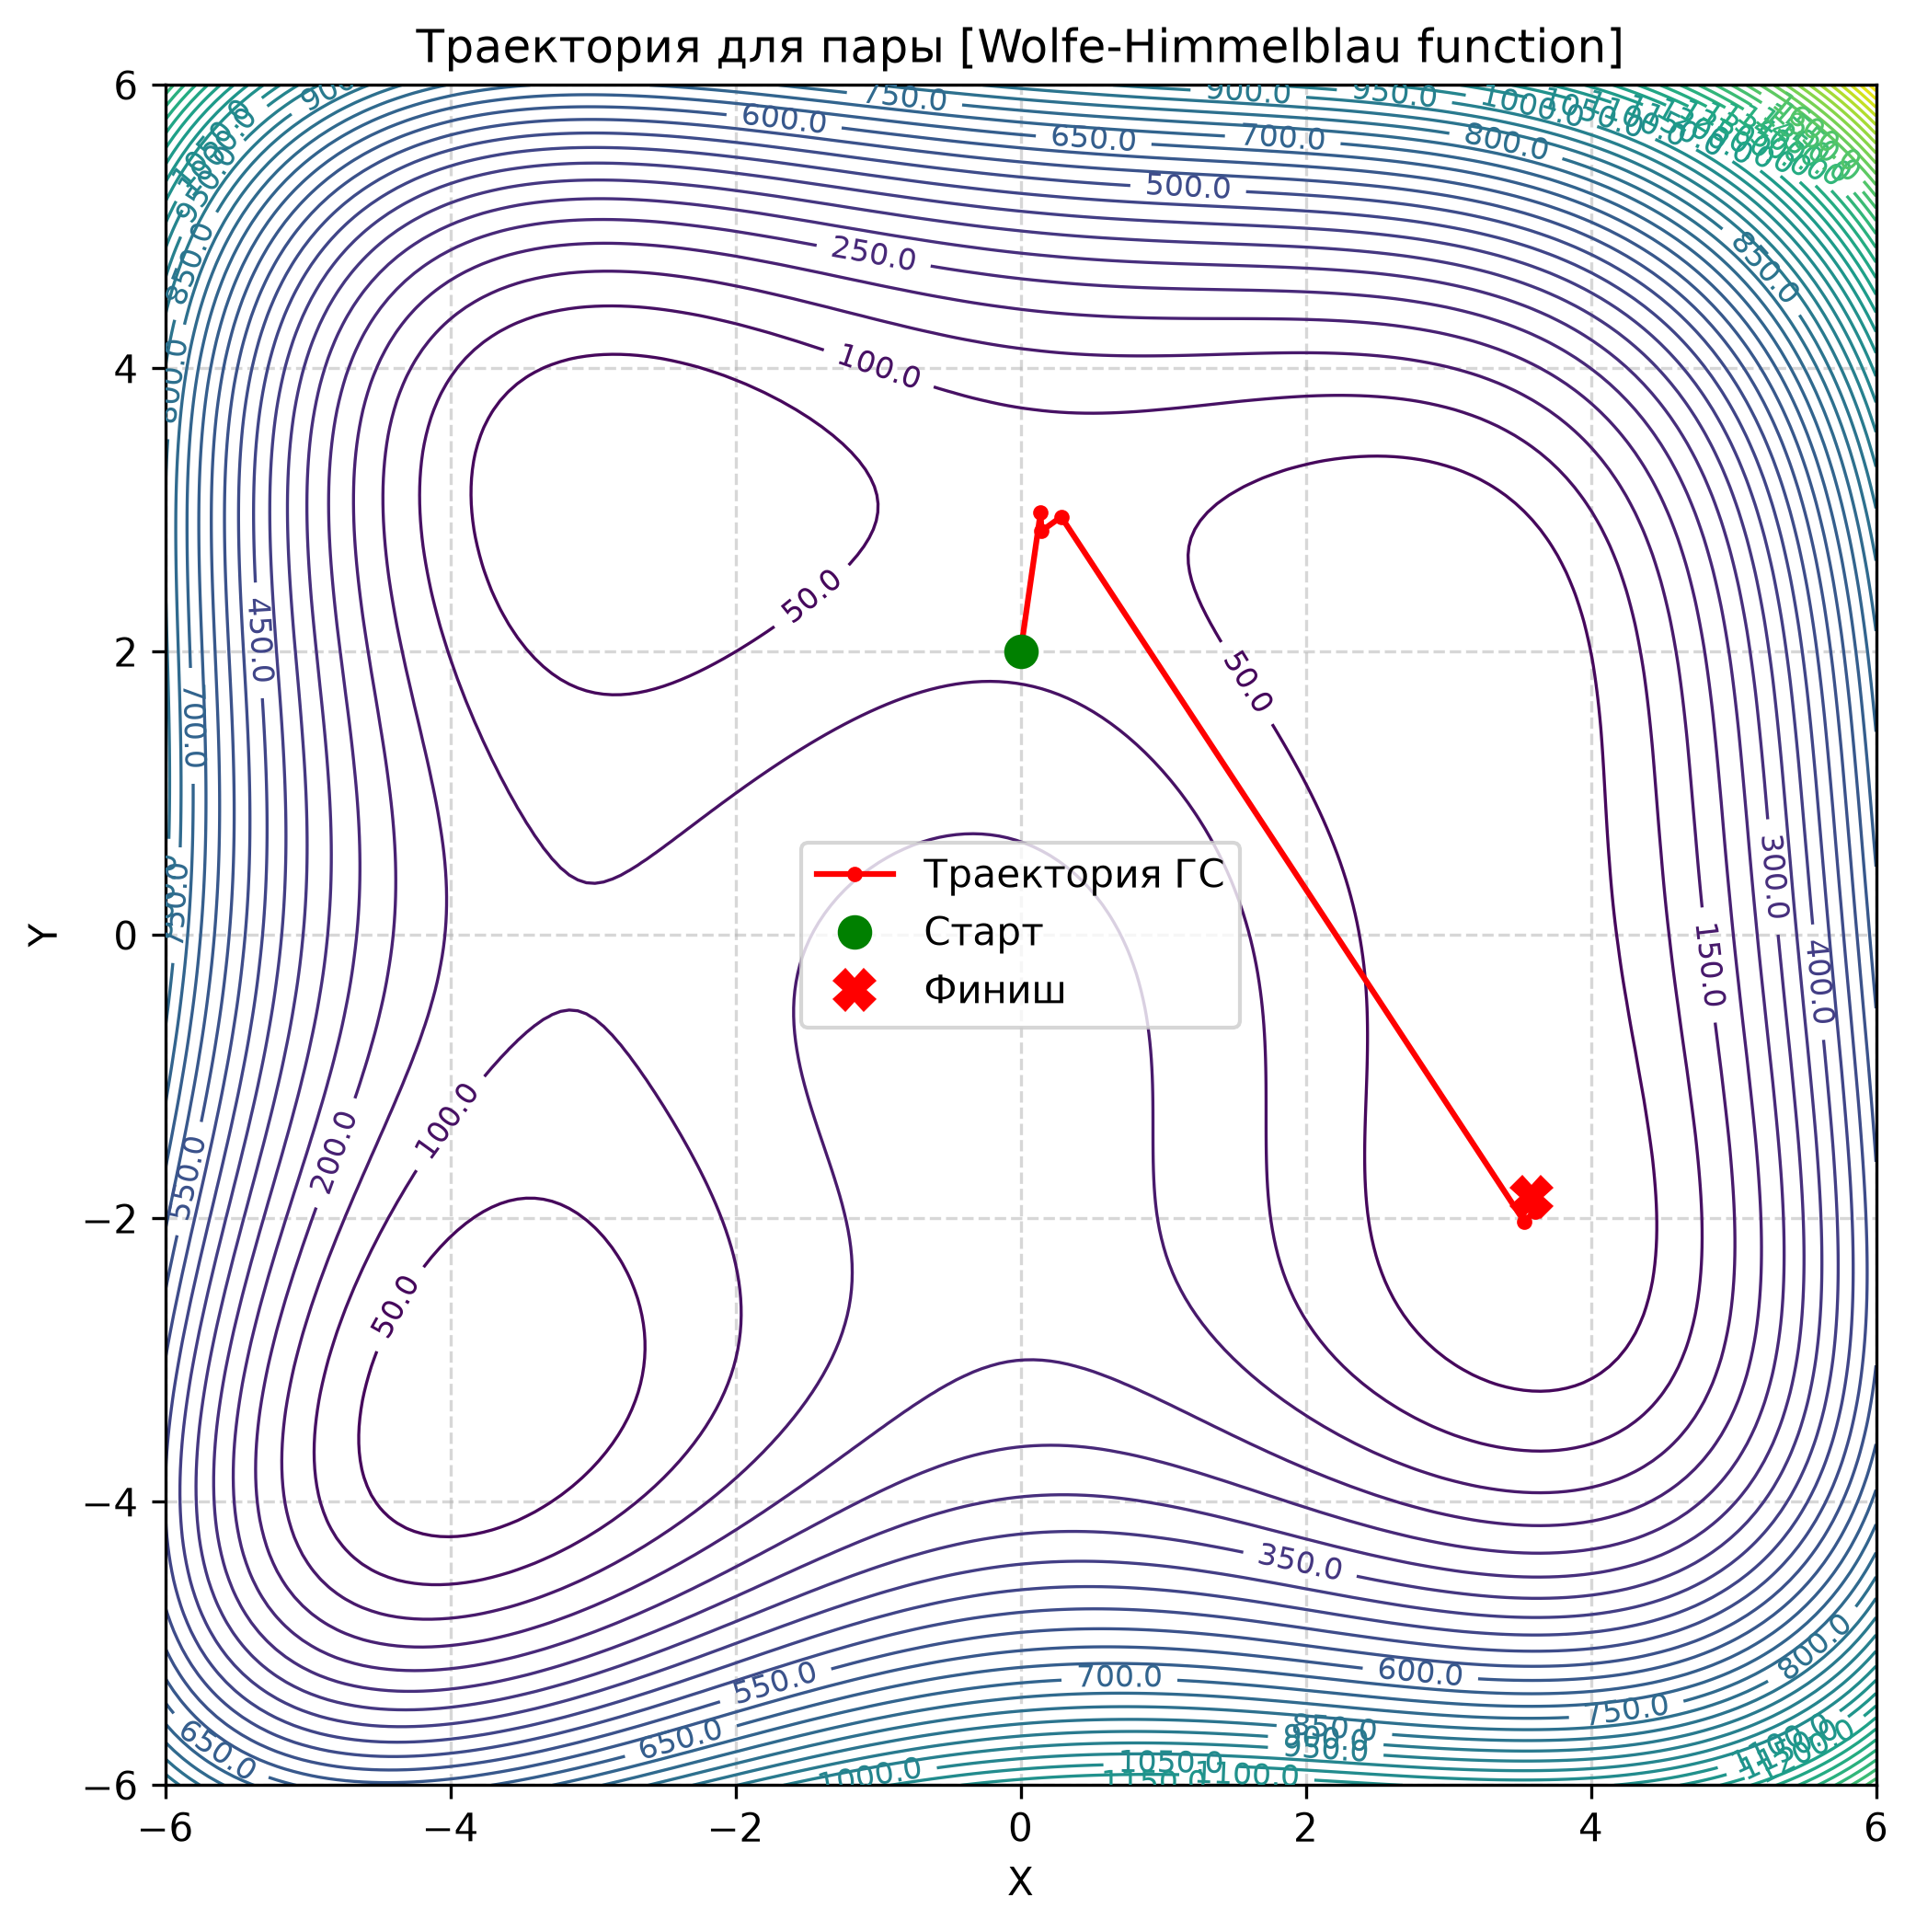
\includegraphics[width=0.49\textwidth]{plot_[Wolfe-Himmelblau function]_Point(0.0, 2.0)_Trajectory.png}}%
%\hfill % <-- Seperation
\subcaptionbox{Нач. точка (-1,3)}{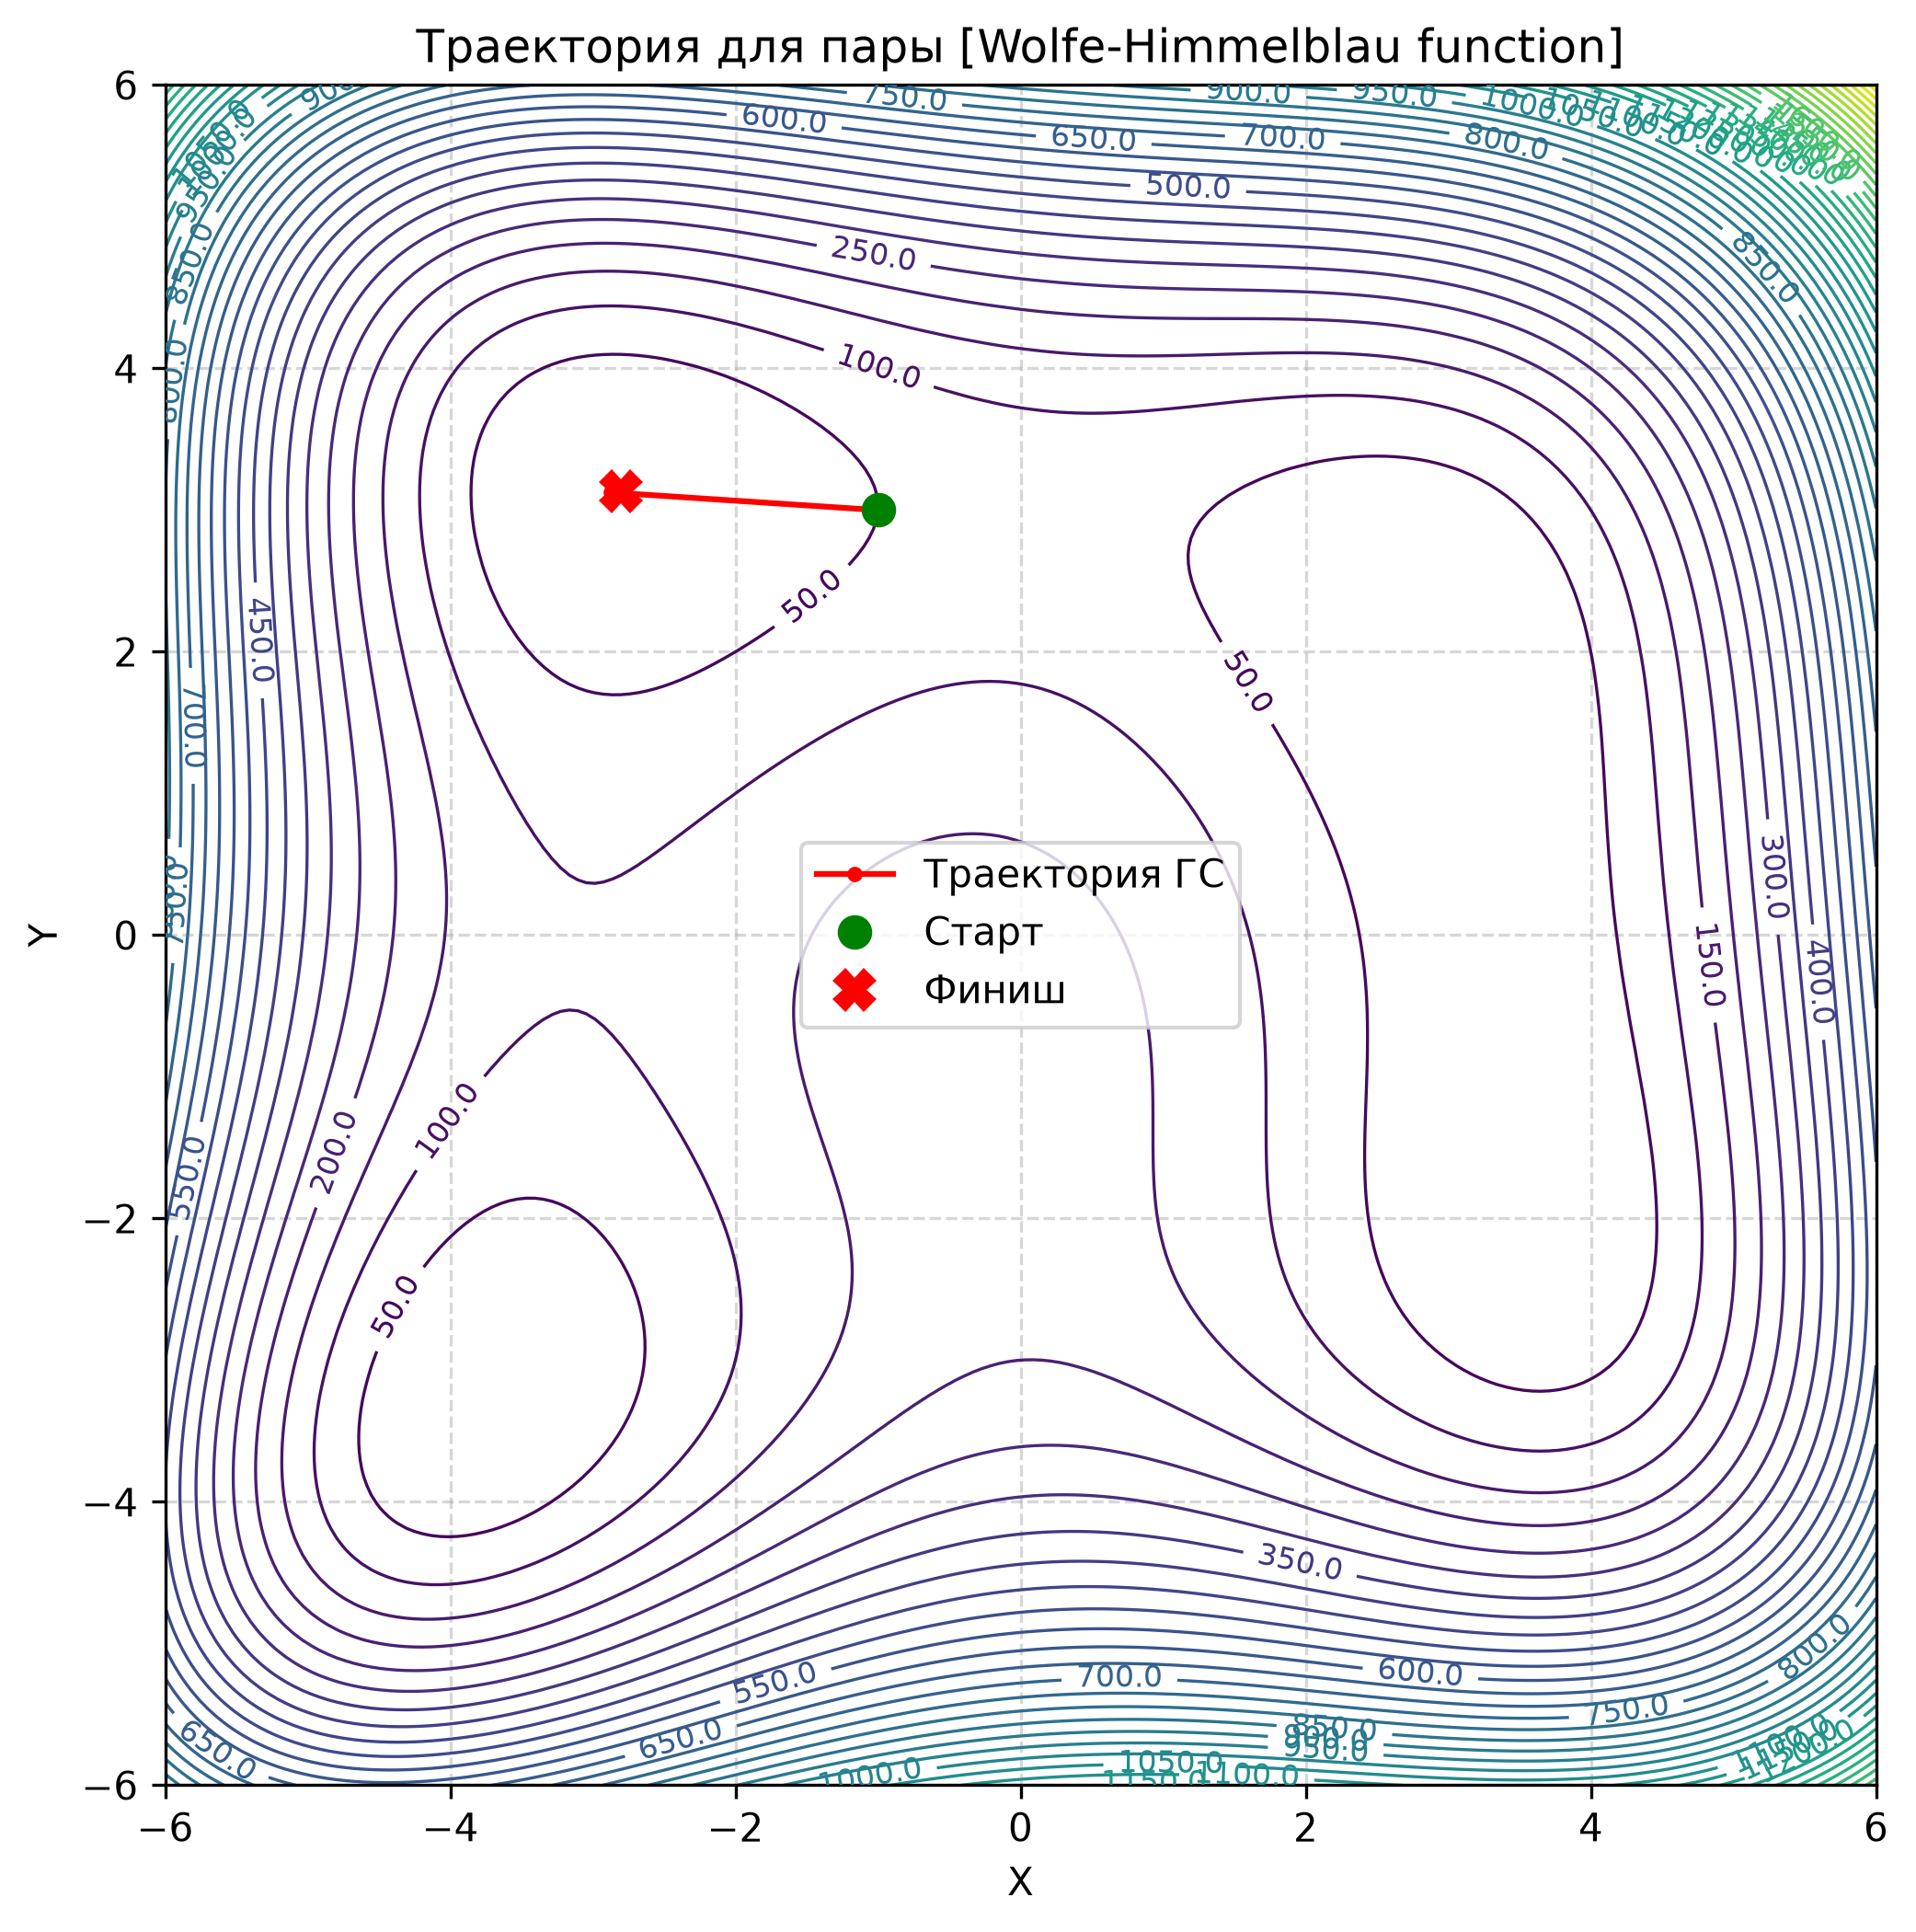
\includegraphics[width=0.5\textwidth]{plot_[Wolfe-Himmelblau function]_Point(-1.0, 3.0)_Trajectory.png}}%
\caption{Сильные условия Вольфе для функции Химмельблау. Траектория алгоритма.}
\end{figure}

В случае же функции Экли сходимость алгоритмов к глобальному минимуму было делом удачи и только:

\begin{figure}[H]
\centering
\subcaptionbox{Сходящийся Вольфе}{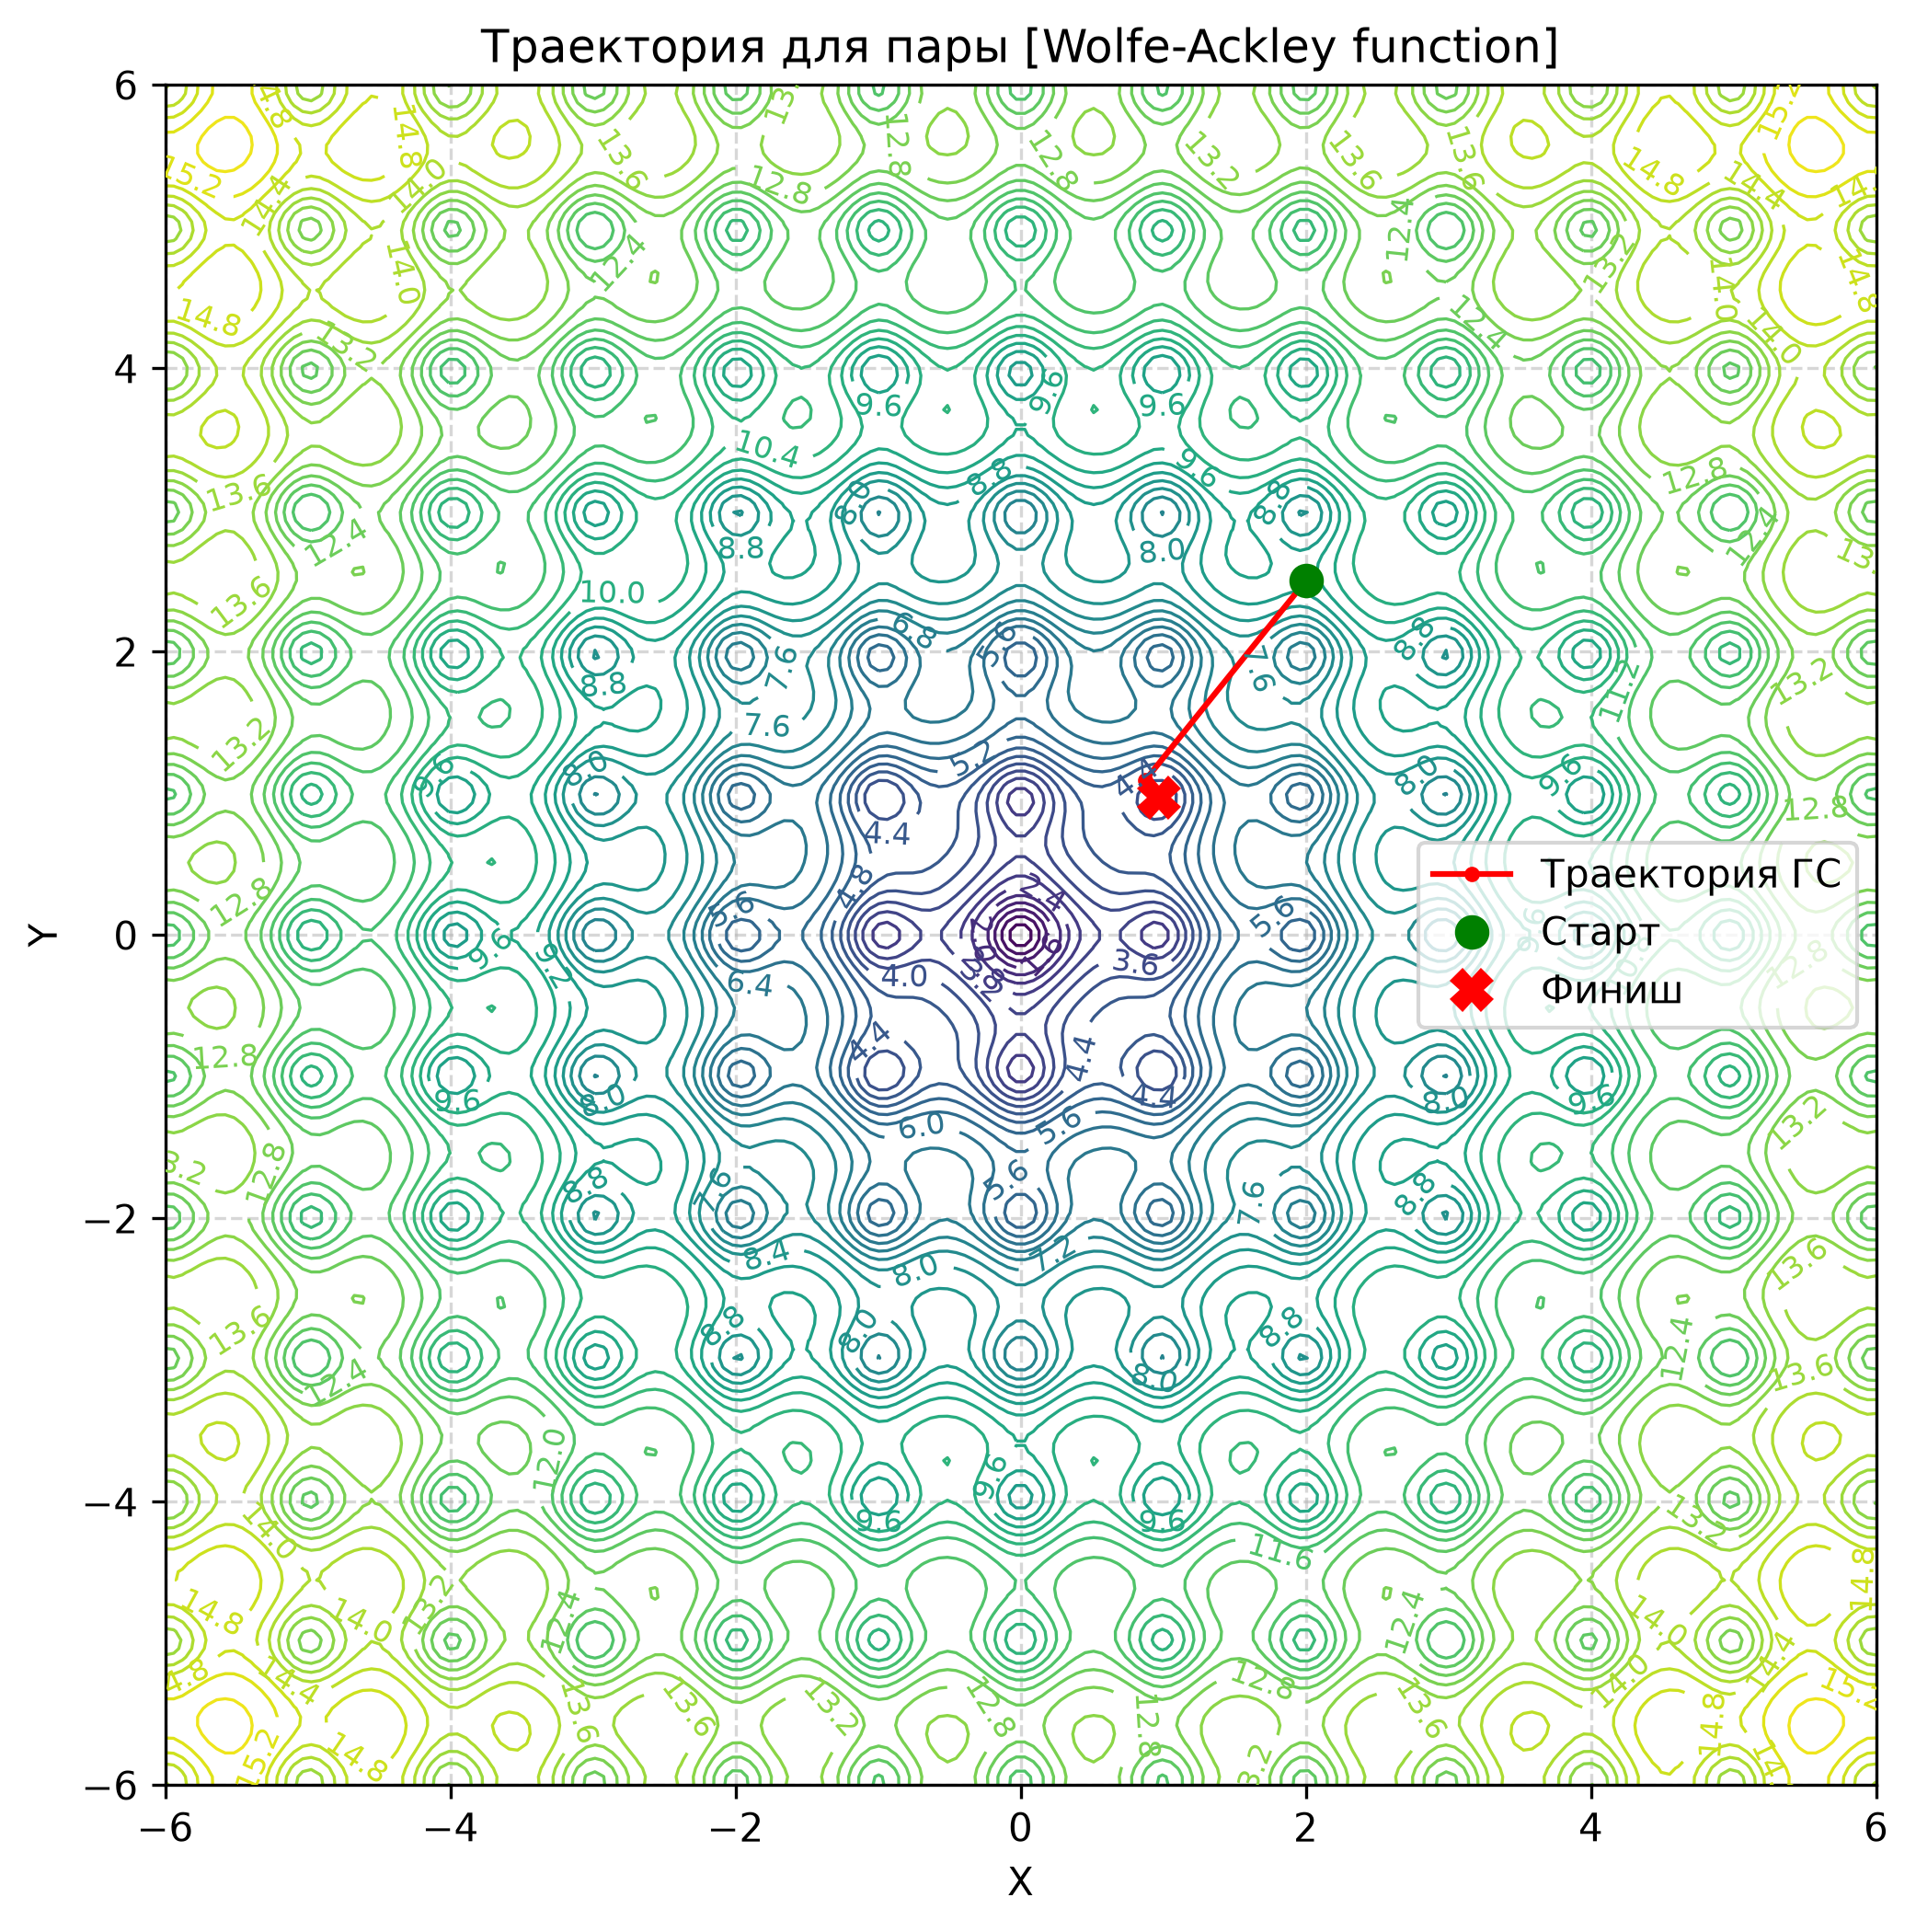
\includegraphics[width=0.49\textwidth]{plot_[Wolfe-Ackley function]_Point(2.0, 2.5)_Trajectory.png}}%
%\hfill % <-- Seperation
\subcaptionbox{Несходящийся Вольфе}{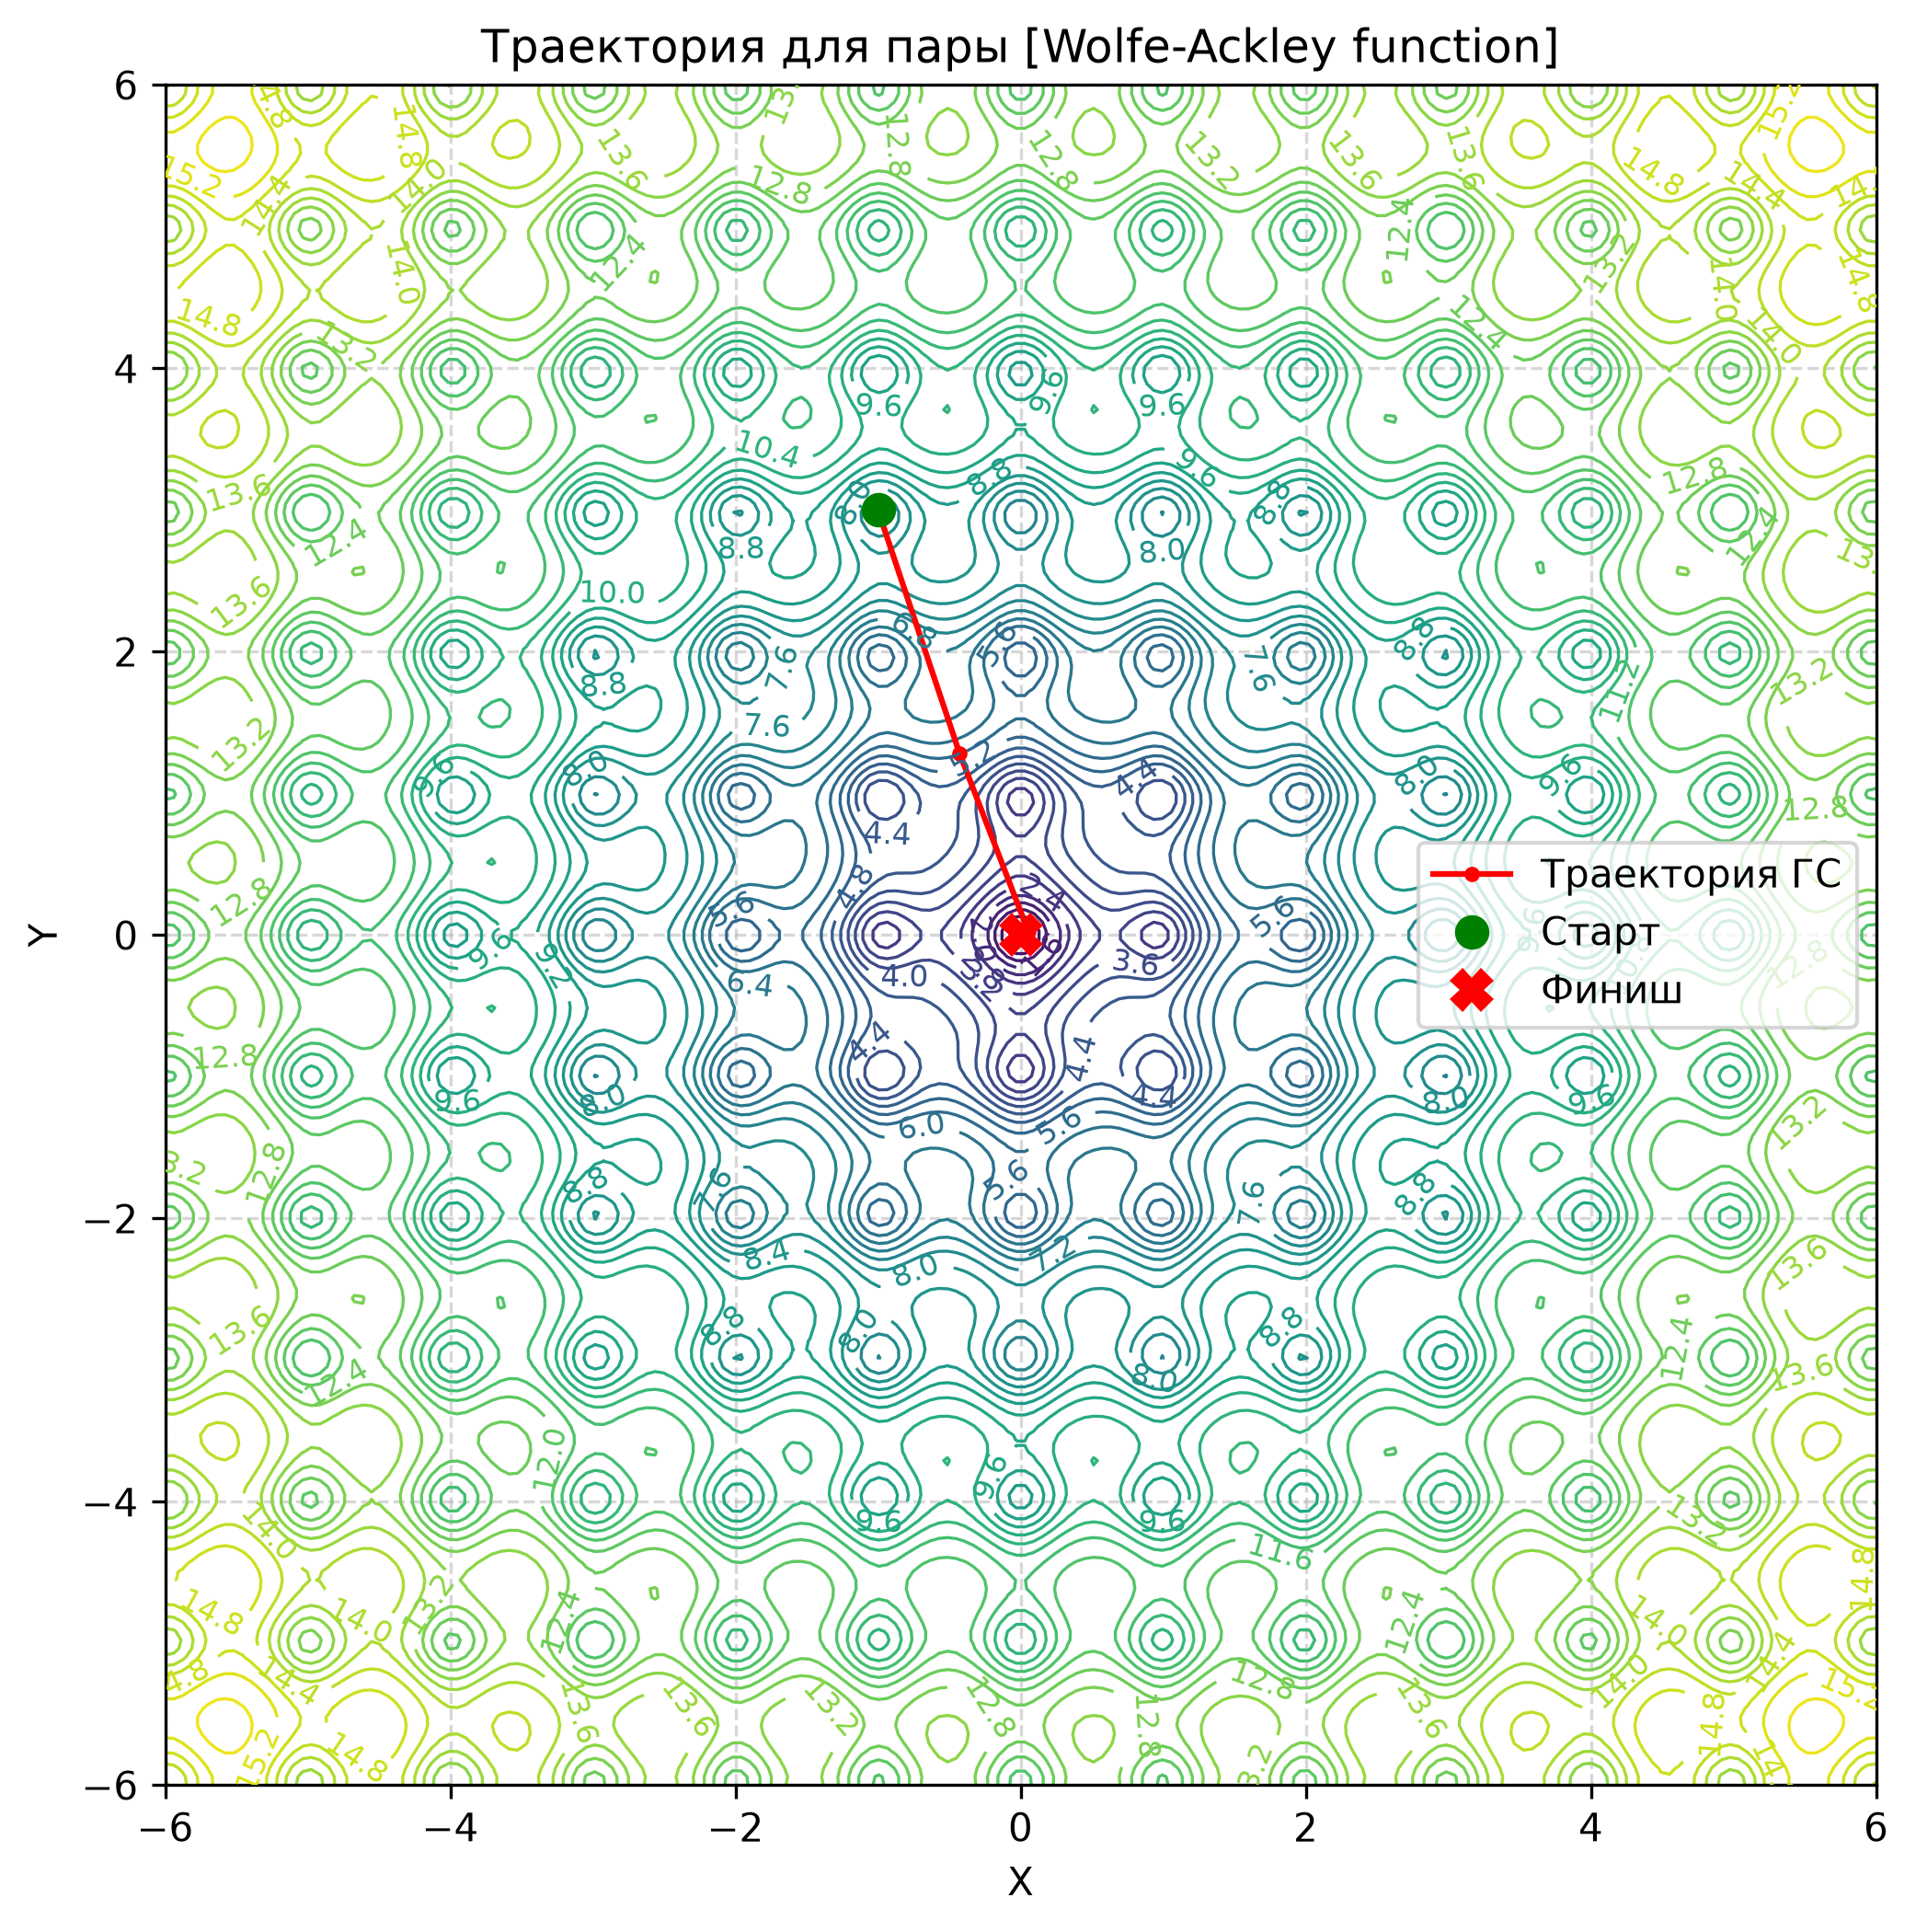
\includegraphics[width=0.5\textwidth]{plot_[Wolfe-Ackley function]_Point(-1.0, 3.0)_Trajectory.png}}%
\caption{Сильные условия Вольфе для функции Экли. Траектория алгоритма.}
\end{figure}

\subsubsection{Сходимость метода наискорейшего спуска}

\begin{figure}[H]
    \centering
    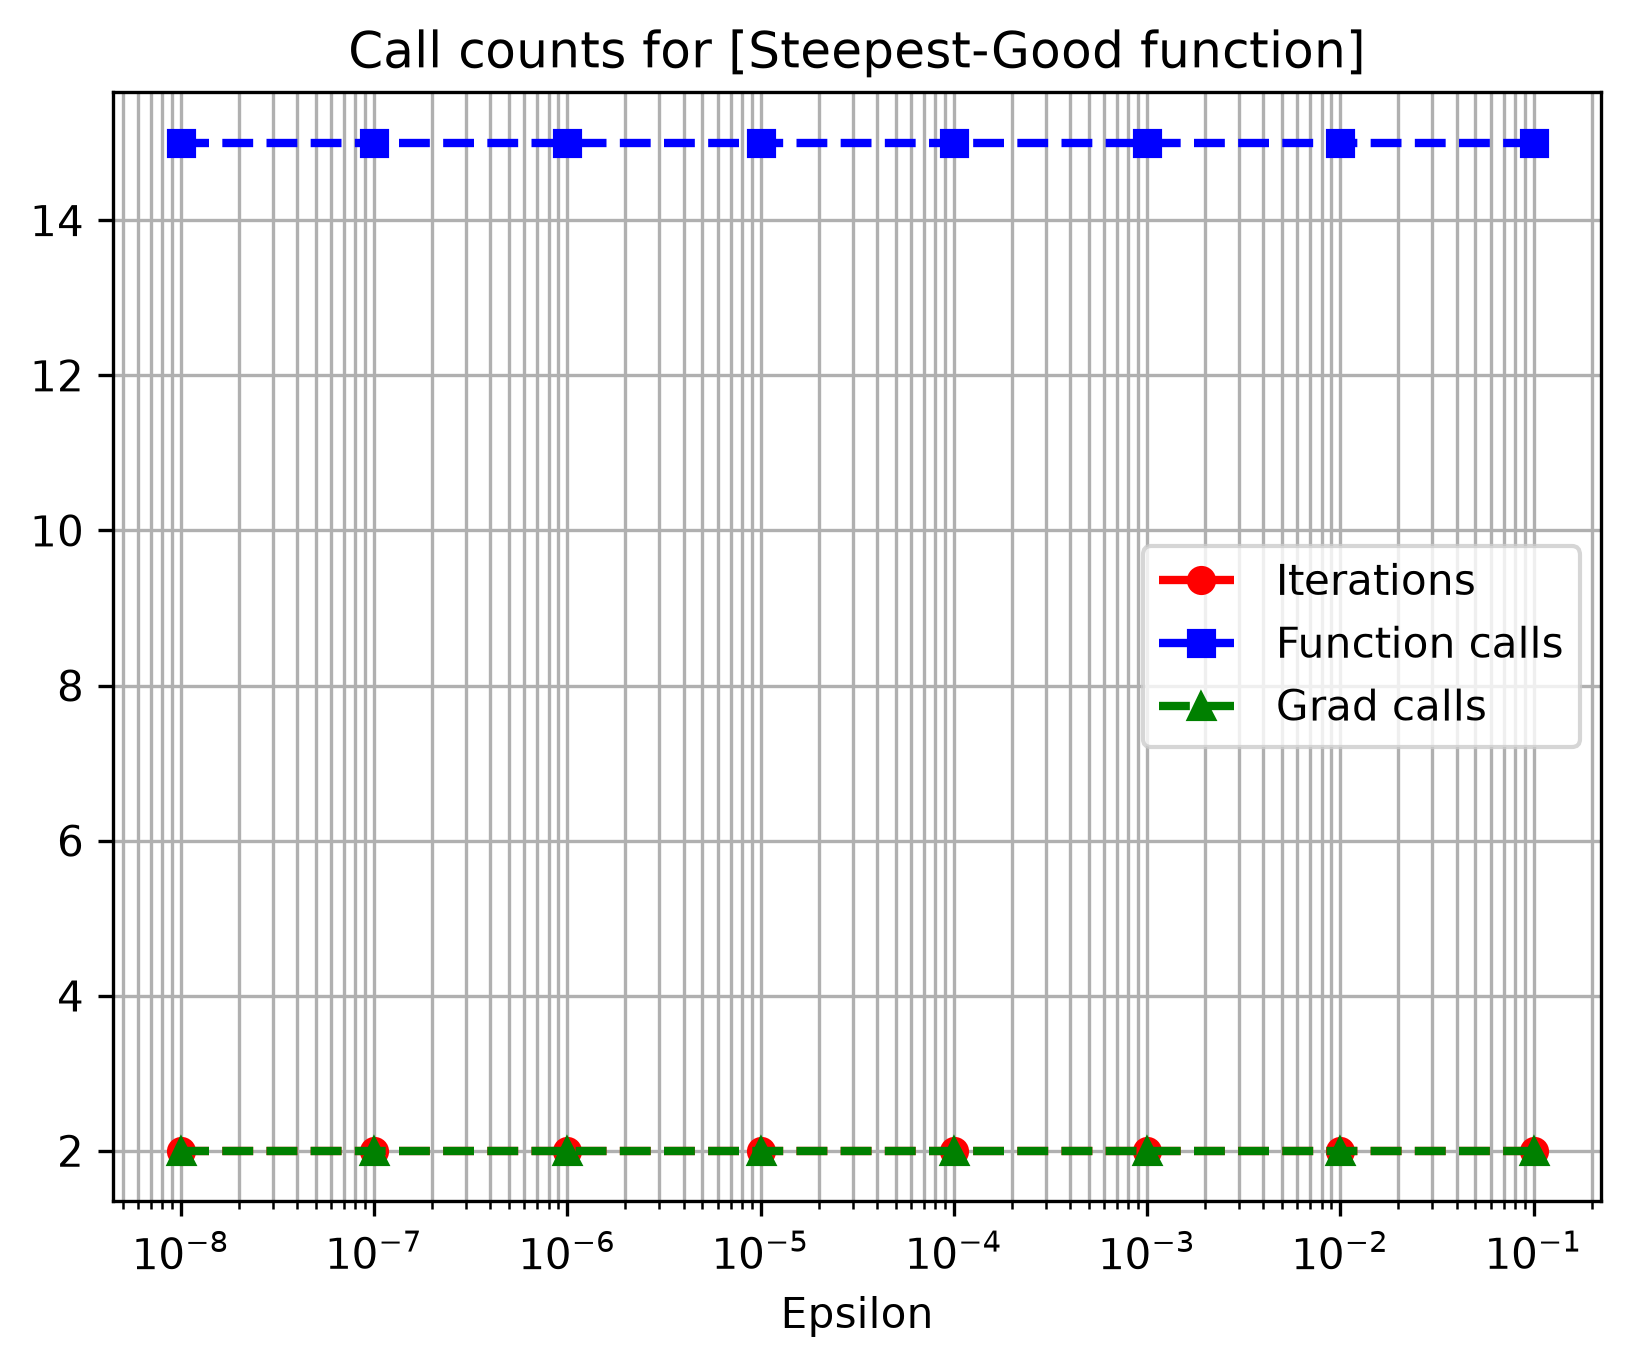
\includegraphics[width=0.5\linewidth]{task6_[Steepest-Good function]_table.png}
    \caption{Метод наискорейшего спуска для хорошей функции}
\end{figure}
\begin{figure}[H]
    \centering
    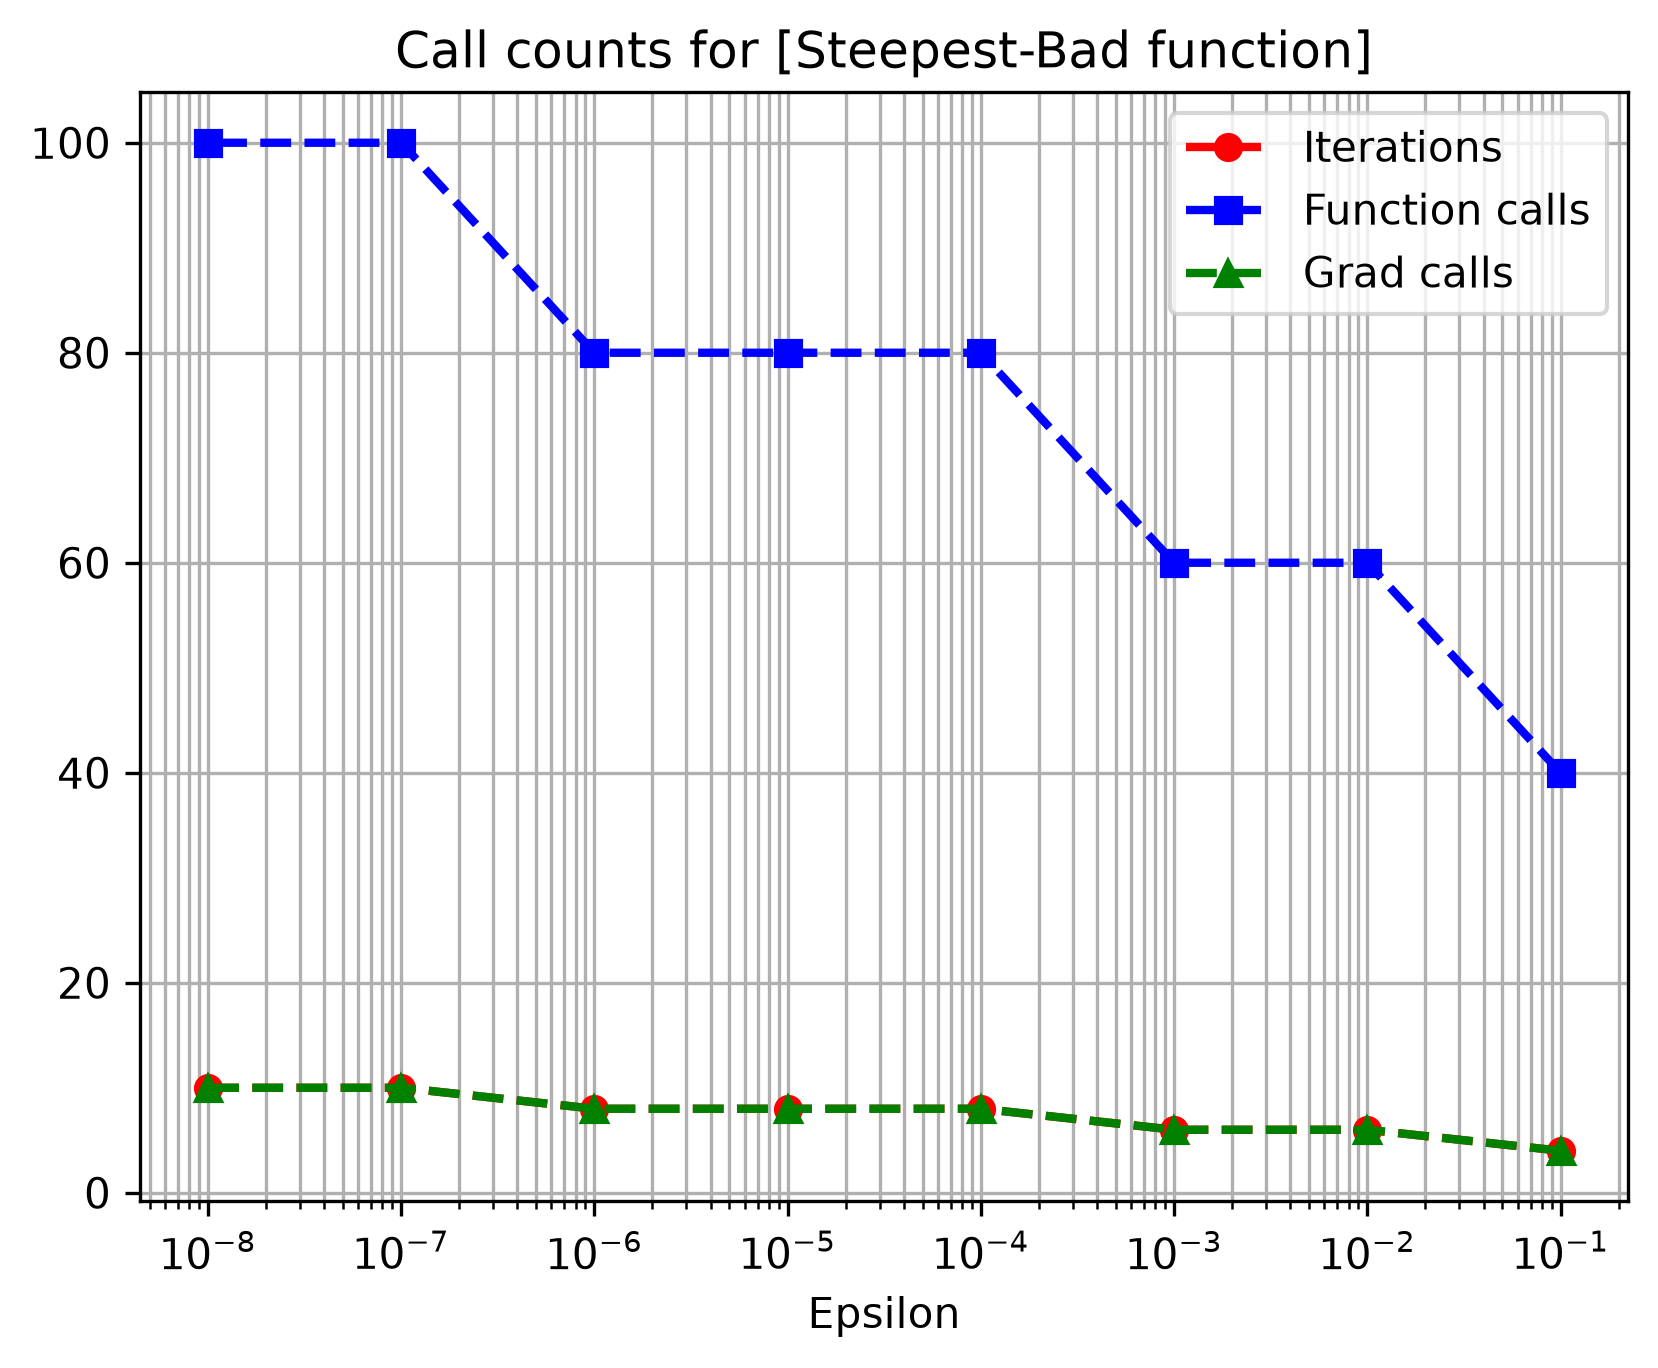
\includegraphics[width=0.5\linewidth]{task6_[Steepest-Bad function]_table.png}
    \caption{Метод наискорейшего спуска для плохой функции}
\end{figure}

Заметим, что метод наискорейшего спуска очень эффективно справляется с поиском минимума. В случае хорошей функции это объясняется тем, что функция симметрична, и её градиент уже направлен от минимума. В случае плохой функции алгоритм быстро выходит на ось $OX$, после чего рассуждения аналогичны.

Также заметим, что метод наискорейшего спуска удачно справляется с поиском минимума для всех сложных функций (\textbf{даже для функции Экли!}), вне зависимости от начального положения запуска. Однако не все так однозначно: так, для функции Розенброка, методу требуется астрономическое количество вызовов функции для нахождения минимума:

\begin{table}[!ht]
    \centering
    \begin{tabular}{|c|c|c|c|c|}
    \hline
        {P\_x} & {P\_y} & {N\_Iter} & {F\_Call\_Count} & {Grad\_Call\_Count} \\ \hline
        2.0 & 2.5 & 4178 & 105357 & 4178 \\ \hline
        3.0 & 3.0 & 8208 & 208204 & 8208 \\ \hline
        4.0 & 1.0 & 8244 & 203237 & 8244 \\ \hline
        0.0 & 2.0 & 10000 & 221149 & 10000 \\ \hline
        -1.0 & 3.0 & 10000 & 230245 & 10000 \\ \hline
    \end{tabular}
    \caption{Метод наискорейшего спуска для функции Розенброка (предел итераций 10000).}
\end{table}

\section{Выводы и анализ результатов работы}

Были реализованы и исследованы методы градиентного спуска для минимизации многомерных функций. Проведен подробный анализ поведения моделей оптимизаторов при различных конфигурациях задач. Подтверждена точность математической модели оптимизаторов. Изучено асимптотическое поведение оптимизаторов и их сходимость. Выявлены функции, на которых некоторые оптимизаторы не находят минимум за разумное время.

\end{document}
